% !TEX TS-program = pdflatexmk
% !TEX spellcheck = language_tag
\documentclass[fleqn,usenatbib]{mnras}

\usepackage[T1]{fontenc}
\usepackage{ae,aecompl}

\usepackage{graphicx}
\usepackage{amsmath}
\usepackage{amssymb}
\usepackage{newtxtext,newtxmath}

\usepackage{multirow}
\usepackage{array}
\usepackage{xcolor}
\usepackage{ulem}
\usepackage{xspace}

% ABBREVIATIONS
\newcommand{\ud}{\ensuremath{\mathrm{d}}\xspace}
\newcommand{\tpb}{\ensuremath{t_{\text{pb}}}}

\newcommand{\helium}{\ensuremath{\mathrm{^{4}He}}\xspace}
\newcommand{\nickel}{\ensuremath{\mathrm{^{56}Ni}}\xspace}
\newcommand{\tracer}{\ensuremath{\mathrm{Tr}}\xspace}
\newcommand{\ye}{\ensuremath{Y_{e}}\xspace}
\newcommand{\iron}{\ensuremath{\mathrm{^{56}Fe}}\xspace}
\newcommand{\cobalt}{\ensuremath{\mathrm{^{56}Co}}\xspace}

\newcommand{\solr}{\ensuremath{\rm{R_{\odot}}}\xspace}
\newcommand{\solm}{\ensuremath{\rm{M_{\odot}}}\xspace}
\newcommand{\mns}{$M_{\mathrm{NS}}$}
\newcommand{\rsh}{$R_{\text{s}}$}
\newcommand{\rrevsh}{$R_{\mathrm{revs}}$}
\newcommand{\rgain}{$R_{\mathrm{gain}}$}

\newcommand{\kms}{\ensuremath{\mathrm{km\, s^{-1}}}}
\newcommand{\km}{\ensuremath{\mathrm{km}}}
\newcommand{\s}{\ensuremath{\text{s}}}
\newcommand{\ms}{\ensuremath{\text{ms}}}
\newcommand{\gcc}{\text{g}\, \text{cm}^{-3}}
\newcommand{\kbpnuc}{k_{\text{b}}/\text{nucleon}}


\newcommand{\prom}{\textsc{Prometheus-HOTB}\xspace}
\newcommand{\vertexprom}{\textsc{Vertex-Prometheus}\xspace}
\newcommand{\vertex}{\textsc{Vertex}\xspace}
\newcommand{\nada}{\textsc{NADA-FLD}\xspace}
\newcommand{\rns}{\ensuremath{R_{\mathrm{NS}}}\xspace}

%keeping track of changes
\newcommand{\NY}[2]{{\color{blue}\sout{#1}#2}}
\newcommand{\GEO}[2]{{\color{red}\sout{#1}#2}}
\newcommand{\COM}[1]{{\color{orange}#1}}

\title{Three-dimensional Models of Core-collapse Supernovae from Low-mass Progenitors}

\author[G. Stockinger et. al]{
 G.~Stockinger$^{1,2}$\thanks{Email: georgsto@mpa-garching.mpg.de},
 H.-T.~Janka$^1$,
 T.~Ertl$^1$,
 D.~Kresse$^1$,
 K.~Nomoto$^3$,
 A.~Heger$^{4,5,6}$,\and
 A.~Gessner$^7$
 \\
% Institutions
$^1$Max Planck Institute for Astrophysics, Karl-Schwarzschild-Str.1 , D-85748 Garching, Germany\\
$^2$Physik Department, Technische Universit\"at M\"unchen, James-Franck-Stra{\ss}e 1, D-85748 Garching, Germany\\
$^3$Kavli Institute for the Physics and Mathematics of the Universe (WPI), The University of Tokyo Institutes for Advanced Study,\\  \hspace{0.08cm} The University of Tokyo, Kashiwa, Chiba 277-8583, Japan\\
$^4$School of Physics \& Astronomy, University of Minnesota, Minneapolis, MN-55455, USA \\
$^5$Center for Nuclear Astrophysics, Department of Physics \& Astronomy, Shanghai Jiao-Tong University, Shanghai-200240, P. R. China \\
$^6$Joint Institute for Nuclear Astrophysics, 1 Cyclotron Laboratory, National Superconducting Cyclotron Laboratory, Michigan State University,\\ \hspace{0.08cm} East Lansing, MI-48824-1321, USA \\
$^7$Max Planck Institute for Intelligent Systems, Max-Planck-Ring 4, D-72076 T\"ubingen, Germany \\
}

\date{Released 2019 Xxxxx XX}

% Enter the current year, for the copyright statements etc.
\pubyear{2019}

\begin{document}
\label{firstpage}
\pagerange{\pageref{firstpage}--\pageref{lastpage}}
\maketitle
\pubyear{2019}

\begin{abstract}
We present the results of full $4\pi\mathord{-}$3D, long term simulations of core-collapse supernova (CCSN) resulting from low-mass progenitors, covering the evolution from bounce through shock revival until shock breakout. We consider two low-mass iron-core progenitors with zero metallicity and solar metallicity which explode as CCSNe, and one progenitor with an oxygen-neon-magnesium core which explodes as an electron-capture supernova (ECSN). In the ECSN case, mixing of nickel inefficient because of a relatively spherical beginning of the explosion triggered by a steep density gradient outside of the degenerate core concomitant with the absence of secondary non-radial instabilities at composition-shell interfaces of the progenitor. The similarity between the core structure of the zero-metallicity progenitor and the ONeMg progenitor leads to similarities in their explosion properties. In both these cases, we observe roughly equal amount of nickel mixing and qualitatively similar ejecta morphology at late times characterized by small deviations from spherical symmetry. In contrast, the solar-metallicity iron-core progenitor shows strong growth of Rayleigh-Taylor plumes in the entire helium core. The large initial asymmetries lead to more pronounced mixing. In this case the final morphology is remarkably similar to the remnant morphology seen in long term simulations of massive progenitors.
\end{abstract}

\begin{keywords}
  supernovae: general -- stars: massive -- stars: neutron
\end{keywords}

\noindent

\section{ToDo}
\begin{itemize}
    \item Nickel velocities
    \item $s9.0$ multi D description
    \item Comparison other studies
    \item Description 1D shorter ?
\end{itemize}

\section{Introduction}
\NY{}{COMMENT: 1.Use shorter sentences 2. Use citealt when you cite a lot of works inside (see e.g. blah-blah-blah). 3. When citing multiple papers they should go in a time order.}

\NY{}{COMMENT: SINCE YOU STARTED THE PAPER BY DISCUSSING IRON-CORE PROGENITORS AND THEN ONEMG CASE, MAINTAIN THE ORDER IN ALL THE FOLLOWING DISCUSSION. IT IS IMPORTANT FOR THE COHERENCE OF THE STORY.}
According to current understanding stars with mass $\mathord{\gtrsim}\,8\, \solm$ end their lives in a core-collapse supernova. The explosion is powered by gravitational energy, which is released when the core of the star collapses to a compact remnant (a neutron star or black hole). In the past six decades numerous studies have focused on the collapse phase and subsequent evolution using 1D simulations. Over the past two decades, multi-dimensional simulations with better treatment of the micro-physics have driven our understanding of the core-collapse problem (see e.g. \citealt{Janka2012,Burrows2013,Janka2016}). A close study of these models has lead to the discovery of new hydrodynamic instabilities such as standing accretion shock instability (SASI) (\citealt{Blondin2003,Foglizzo2007}). The increase in computational capabilities in the recent years along with new developments in neutrino transport algorithms (see e.g. \citealt{Sumiyoshi2012,Sumiyoshi2015,Glas2019} and references therein) has resulted in full 3D simulations (see e.g. \citealt{Melson2015a,Summa2016,Vartanyan2018,Melson2019,Vartanyan2019}). Motivated by the historical SN1987A and its progenitor detection, a variety of studies (e.g. \citealt{Mueller1991,Kifonidis2003,Hammer2010,Wongwathanarat2015}) also investigated the propagation of the shock wave from its neutrino-driven initiation to the breakout of the shock from the stellar surface, in 15-20 $\solm$ models, which are suitable as progenitors for SN1987A, in two and three dimensions. 
These theoretical works showed that supernova explosions are by far not spherical events as previously thought. Three dimensional effects may even facilitate explosions \citep{Herant1994a,Burrows1995,Janka1996,Melson2015a,Mueller2017}) and are a necessary ingredient to explain the clumpiness and mixing found in photospheric emission \citep{Utrobin2015,Utrobin2017} and spectral analyses of the nebular phase of core collapse events \citep{Jerkstrand2017}. 
\citet{Wongwathanarat2015} show that the final ejecta distribution carries imprint of the 
asphericities produced during the onset of the explosion ($t\,\mathord{\sim}\, 1\, \rm s$), which are further modified during later phases. Depending on the detailed progenitor structure, hydrodynamic instabilities arising at the composition interfaces, such as the Rayleigh-Taylor instability (RTI) shapes the final spatial and velocity distribution of nucleosynthetic products. The resulting ejecta morphology ranges homogenously mixed ejecta to strongly pronounced RT-fingers resembling also the  distribution found in Cas A \citep{Wongwathanarat2017,Grefenstette2017}. Due to the highly complex and stochastic behaviour of turbulence during the onset of the explosion phase and the nonlinear evolution of the RTI a clear connection between the asymmetries, and thus the amount of mixing, and the progenitor structure has still to be worked out.

In this paper we consider CCSN progenitors with lowest masses, where up to 40\% of all CCSNe are thought to occur (assuming Salpeter initial mass function  \citep{Salpeter1955} and an upper mass limit of $\mathord{\sim}10\,\solm$ for CCSNe), to study the differences in their development of mixing instabilities during the explosion. To this end we compare electron-capture SNe (ECSNe) from ONeMg core progenitors and CCSNe from iron care progenitors, all with around $9\,\solm$. 

The evolution of stars with mass $\mathord{\lesssim}\,12\, \solm$ is very sensitive to the initial mass \citep{Woosley2015}.
Iron-core CCSN progenitors with masses around $9\mathord{-}10\,\solm$ go through a phase of oxygen and silicon burning that is longer in comparison with their more massive ($M \mathord{>} 15\, \solm$) counterparts. This can lead to additional mass loss in the last decade of evolution or even to single mass ejection events when burning flames reach the surface of the star before collapse \citet{Woosley2015}.

The $8.8\, \solm$ progenitor of \cite{Nomoto1984} is even more peculiar. It experiences  several thermal pulses and off-center ignition of fusion material. In the end, it has a degenerate ONeMg core surrounded by a dilute and an extended hydrogen envelope.
 
When the core approaches its Chandrasekhar mass electron captures on $\mathrm{^{24}Mg}$ via the reactions $\mathrm{^{24}Mg(e^-,\nu_e)}^{24}\mathrm{Na}$  and $\mathrm{^{24}Mg(e^-,\nu_e)}^{24}\mathrm{Ne}$ destabilize the core due to the reduction of electron-degeneracy pressure. Continuous $e^-$-capture on $\mathrm{^{20}Ne}$ that further reduces supporting pressure works against the now beginning oxygen-burning as temperatures increase during the collapse. Simulations in 1D (see e.g. \citealt{Kitaura2006,Janka2008}) suggest that the collapse proceeds despite the oxygen burning. \cite{Jones2016} simulated the deflagration of oxygen in ONeMg cores with different core densities. Below $\log_{10}\rho_c=10.3$ their core do not collapse but get partly unbound due to the inefficient semi-convective mixing during the electron capture phase and the resulting strong thermonuclear runaway. Only when central densities are higher than $\rho_c$ the core is found to collapse to a proto-neutron star (PNS).
Recently, \cite{Kirsebom2019} investigated the influence of a newly measured rate of a strong transition between the ground states of $^{20}\mathrm{Ne}$ and $^{20}\mathrm{F}$ on the evolution of ONeMg core. Adding the new transition increases the likelihood that the star is (partially) disrupted by a thermonuclear explosion rather than collapsing to form a PNS. \COM{Effect on this study?}

Despite the narrow mass range and competing processes that depend strongly on the employed physics, some suggestions for ECSNe  are SN 1994N, 1997D, 1999br, 1999eu, 2011dc and 2005cs \citep{Stevenson2014}. Also SN1054 (the Crab) has been suggested to be an ECSN although it is in conflict with results by \citep{Gessner2018} concerning the maximum kick velocity of PNS's produced by ECSNe.

In this work we attempt to investigate the following questions with the help of fully three-dimensional simulations:
\begin{itemize}
\item  What are the major differences between the long term evolution of an ECSNe and a CCSNe?
\item What is the influence of the progenitor structure on shock propagation, reverse shock formation and mixing of neutrino heated material?
\item Can these differences be detected without detailed spectral analysis?
\end {itemize}

\section{Progenitors}
% pre collapse 
\textbf{In this paper, we study an ECSN of a non-rotating 8.8 \solm progenitor ($e8.8$) \citetext{Nomoto, 2017, private communication} and two non-rotating CCSNe resulting from low-mass iron-core progenitors ($z9.6$, $s9.0$), provided by A. Heger \citetext{2015, private communication} \citep{Woosley2015} and \cite{Sukhbold2016}, respectively. The considered ECSN progenitor is explored here for the first time whereas the explosion of iron-core progenitors was simulated in 3D with the \vertexprom code and are published in \cite{Melson2015a} and \cite{Melson2019}. }

\subsection{ESCN progenitor}
The $e8.8$ model is a solar metallicity progenitor with a ZAMS mass of $M_{\rm ZAMS}\mathord{=}8.8\,\solm$ and was provided by Nomoto \citetext{2017, private communication}. This progenitor has an ONeMg core, which explodes as an ECSN. 
It has the typical very sharp density gradient outside of its $1.33\, \solm$ ONeMg core ($\xi_{2.5}\mathord{=}5.7\times10^{-6}$, $\xi_{1.5}\mathord{=}8.0\times10^{-6}$)\footnote{Because of its relevance for higher-mass progenitors we provide the compactness parameter \citep{OConnor2011} {$\xi_{M}\equiv \frac{M/\solm}{R(M_{\rm bary}\mathord{=}M)/10^{3}\, \rm km}$}. Due to the steep density gradient outside of the core of the considered progenitors, its significance in the present context is, however, questionable.} which can be seen from the density ($\rho$) profile in Figure~\ref{fig:prog_tem_rho_ye_rhor}, where we also show the $\rho r^3$-profiles, besides the electron fraction $Y_{\mathrm{e}}$ and temperature $T$ as functions of enclosed mass and radius. The dash-dotted, dashed and dotted lines indicate the positions of the composition interfaces, degenerate core/CO, CO/He and He/H, respectively. 
\textbf{We define the locations of the composition interfaces, similar to \cite{Wongwathanarat2015}, as those positions at the bottom of the respective layers of the star where the mass fractions $X_{i}$ drop below half of their maximum values in the layer. The radial positions of the composition interfaces are summarized in Table~\ref{tab:progenitors}.}
In the top panel of Figure~\ref{fig:composition_all} we present the composition of model $e8.8$, where we combine all elements with mass number greater than 28 into the ``iron-group'' (IG).
The ONeMg-core is surrounded by a very thin carbon-helium shell ($M_{\rm C}\,\mathord{\approx}\, 6.80\mathord{\times}10^{-2}\, \solm$, $M_{\rm He}\,\mathord{\sim}\,10^{-5}\, \solm$) and a hydrogen envelope ($M_{\rm H}\,\mathord{\approx}\, 4.36\, \solm$) extending from $\mathord{0.002}$ to $\mathord{1.19}\mathord{\times}10^{3}\, \solr$.  
\iffalse
Due to the steep density gradient at the edge of the degenerate core, the explosion is triggered by the neutrino-driven mechanism even in self-consistent one-dimensional (1D) simulations \citep{Groote2014,Kitaura2006}. However, explosion energies are fairly low and only about $10^{50}\,\mathrm{erg}$. 
\fi
A previous version of the progenitor \citep{Nomoto1984,Nomoto1987,Nomoto2008}, commonly termed $e8.8$ in the literature and $e8.8_{\mathrm{n}}$ in this publication, has been used in various studies, including nucleosynthesis \citep{Wanajo2018} and PNS kicks \citep{Gessner2018} and is a reference case for supernova simulations of ECSNe. \textbf{The previously used progenitor $e8.8_{\mathrm{n}}$ has a more massive helium core with a mass of $\mathord{\sim} 1.375 \,\solm$, but a smaller hydrogen envelope (see Figure~\ref{fig:prog_tem_rho_ye_rhor}).} The collapse and post-bounce evolution of the new progenitor are computed with \prom as detailed in Section~\ref{sec:Collapse and post-bounce setup in prom}.

\subsection{Progenitors for CCSNe}
As a second progenitor we employ a zero-metallicity $M_{\text{ZAMS}}\mathord{=}9.6\,\solm$ star, termed $z9.6$. It was first used by \citet{Janka2012} and is also considered in other studies such as \citet{Mueller2013,Mueller2018}. This iron-core progenitor is structurally similar to the ECSN model. It also shows a sharp decline of the density at the edge of its iron-core enabling low-energy explosions in 1D \citep{Melson2015}. 
Evolved as an extension to \cite{Heger2010}, the pre-SN model develops an iron-core of about 1.30 \solm and has a helium layer of about \textbf{0.33} \solm below a massive hydrogen envelope of $\mathord{\sim}8$ \solm ($\xi_{2.5}\mathord{=}7.65 \times 10^{-5}$, $\xi_{1.5}\mathord{=}2.37 \times 10^{-4}$). As the envelope is not enriched by metals, mass loss played only a negligible role during the star's evolution. This leaves the total mass of the star almost unchanged (see Table~\ref{tab:progenitors}). 
Due to its structure it was one of the first iron-core progenitors that exploded in fully self-consistent 3D simulations by \cite{Melson2015a} with \vertexprom. This result provides the initial state for our investigation. 

Moreover, we investigate a solar-metallicity $M_{\text{ZAMS}} \mathord{=} 9.0 \,\solm$ star, termed $s9.0$, of \citet{Sukhbold2016}. \textbf{Its 1.30 \solm iron-core is surrounded by a silicon shell of 0.016 \solm, a carbon-oxygen layer of 0.068 \solm and a helium shell of 0.169 \solm (see Table~\ref{tab:progenitors})}. The hydrogen envelope extends from 1.57 \solm up to 8.75 \solm ($\xi_{2.5}\mathord{=}3.83 \times 10^{-5}$, $\xi_{1.5}\mathord{=}5.25 \times 10^{-3}$).
This progenitor was chosen to be representative for low-mass CCSNe by \cite{Jerkstrand2018}, who focused on the late-time nebular spectra of the supernova, and by \cite{Glas2019} focusing on the neutrino emission during the explosion. The three-dimensional exploding model for our investigation is provided by \citet{Melson2019} and has also been modeled with \vertexprom. 

Although the progenitors considered in this study have very similar ZAMS masses, their pre-collapse core structures differ strongly (see Figure~\ref{fig:prog_tem_rho_ye_rhor}).
We stress the importance of the $\rho r^3$-profiles of the progenitors as they are decisive for the overall evolution of the explosion \citep{Kifonidis2003,Wongwathanarat2015}. he bahavior of the $\rho r^3$-profile yields important information of the propagation of the shock through the stellar structure because, according to \cite{Sedov1961}, positive gradients of $\rho r^3$ cause shock deceleration, whereas negative gradients cause the opposite. \textbf{Additionally, variations of the shock velocity produce crossing pressure and density gradients behind the shock front near the composition-shell interfaces. Such conditions are essential for Rayleigh-Taylor instabilities as detailed in Section~\ref{sec:Linear stability analysis}, assigning them a crucial role for explaining the high-velocity metal-rich ejecta and the radial mixing of heavy elements \citep{Wongwathanarat2015}.}

The ECSN progenitor exhibits an extremely sharp drop of the $\rho r^3$-profile just outside of the ONeMg core. It is this drop in density that enables fast explosions due to an early, rapid drop of the mass accretion rate and of the corresponding ram pressure at the SN shock \citep{Kitaura2006}. Outside the core, the $\rho r^3$-profile grows monotonically as no other composition interfaces are encountered.
The $z9.6$ progenitor falls into the class of ECSN-like progenitors also in this respect: Similar to the electron-capture progenitor, the $z9.6$ model shows a monotonic growth of the $\rho r^3$-profile outside the CO core, where only a small step in the density profile can be seen at the He/H interface.
Model $s9.0$ on the other hand exhibits strong variations in its $\rho r^3$-profile. Shells of different composition are clearly separated by a negative $\rho r^3$-gradient just before the respective interface. Of particular interest are the CO/He and He/H interfaces. These will have an impact on the long-term evolution of the explosion as will be discussed in Section~\ref{sec:Linear stability analysis}.

\begin{figure*}
 \centering
 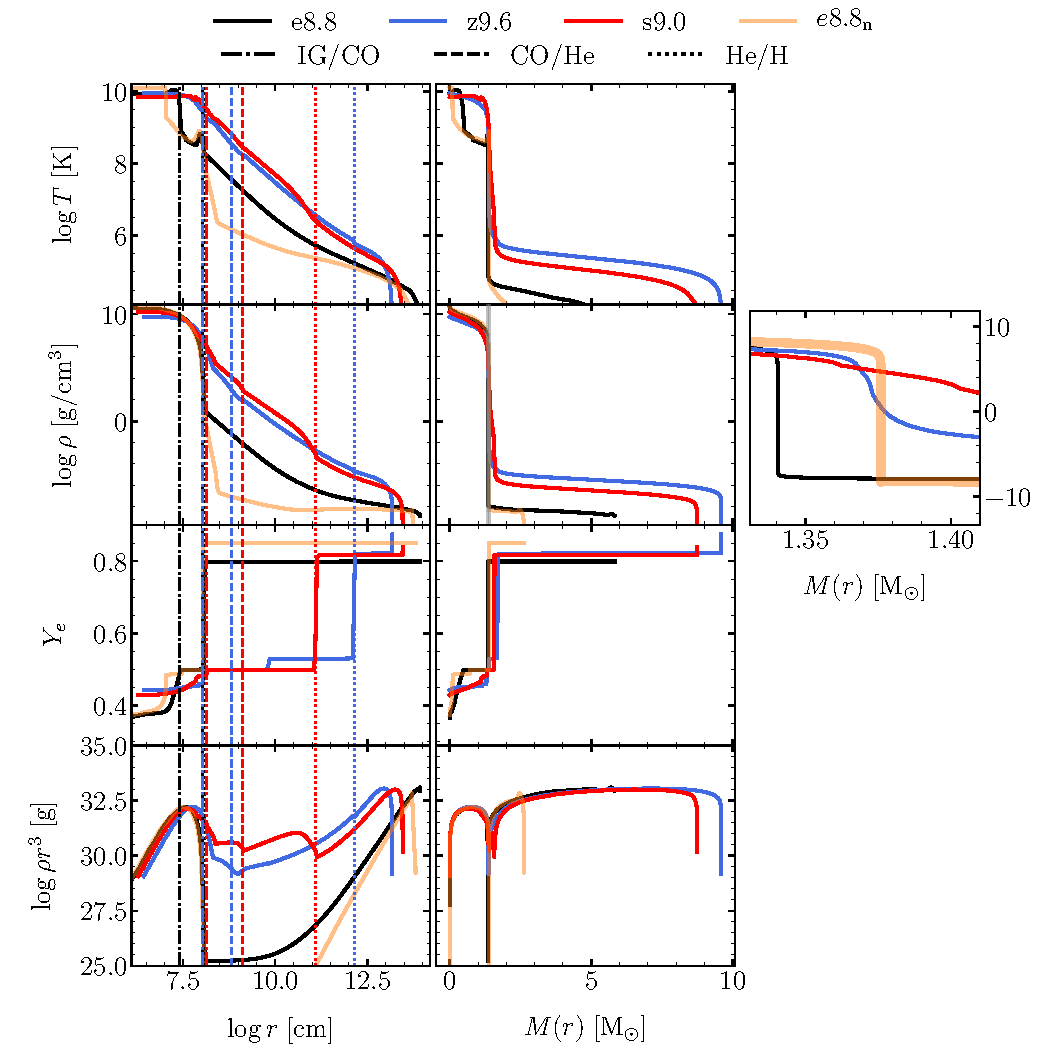
\includegraphics[width=0.9\textwidth,trim=1cm 0.0cm 1cm 0cm]{./pic/progenitors_tem_rho_ye_rhor_paper.pdf}
 \caption{Profiles of the temperature, density, electron fraction ($Y_{\text{e}}$) and $\rho r^3$ for the progenitor models as function of radial coordinate (left panels) and mass coordinate (right panels). Indicated by dashed, dash-dotted and dotted lines are the outer boundaries of the iron-, CO and He cores respectively. Note the huge differences in the density and $\rho r^3$-profiles between the iron and ONeMg cores in particular just outside the CO core. We show the difference in the core structure of our models as a zoom in the $\rho$ vs $M(r)$ profile in the rightmost panel.}
 \label{fig:prog_tem_rho_ye_rhor}
\end{figure*}

For this paper we performed spherically symmetric (1D), axissymmetric (2D) and fully three-dimensional (3D) simulations for all progenitors until the shock reaches the surface of the star. The different setups and approaches for the simulations will be described in the following section.
\begin{figure*}
 \centering
 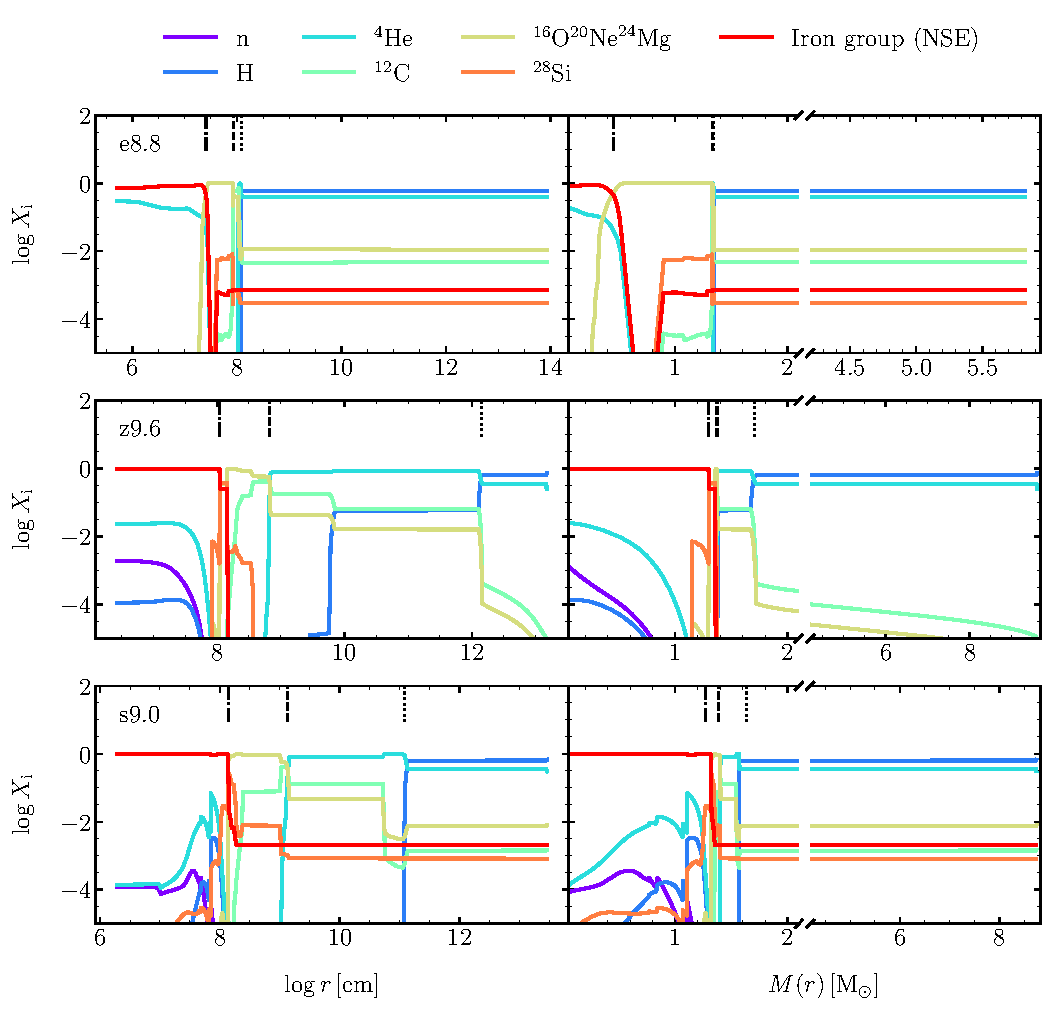
\includegraphics[width=0.9\textwidth,trim=0cm 0.0cm 0cm 0cm,clip]{./pic/composition_all.pdf}
 \caption{Initial pre-collapse composition of the $e8.8$ (top), $z9.6$ (middle) and $s9.0$ (bottom) as a function of radius (left) and enclosed mass (right). We combine all elements with mass number greater than 28 into the ``iron-group'' (IG). The dash-dotted, dashed and dotted lines indicate the the outer boundaries of the iron-, CO and He cores respectively.}
 \label{fig:composition_all}
\end{figure*}

\begin{table*}
   \caption{Shell structure of the pre-collapse progenitor models.}
   \label{tab:progenitors}
   \begin{tabular}{l l l l l} 
   \hline
     Model      &Interface & $\mathrm{R_{shell}\,}$ & $\mathrm{M_{shell}}$ & $t_{\mathrm{sh}}^{\mathrm{3D}}$\\ [0.5ex] 
                &          & [cm] & $[\solm]$ & $[\s]$\\ [0.5ex] 
   \hline
   \multirow{5}{*}{$e8.8$} & IG/ONeMg & $2.57\mathord{\times} 10^{7}$  & 0.45 & - \\ 
                           & ONeMg/C    & $8.48\mathord{\times} 10^{7}$  & 1.33 & 0.15 \\
                           & C/He       & $1.09\mathord{\times} 10^{8}$  & 1.34 & 0.17 \\
                           & He/H       & $1.21\mathord{\times} 10^{8}$  & 1.34 & 0.18\\
                           & Surface    & $8.43\mathord{\times} 10^{13}$ & 5.83 & $4.3\mathord{\times}10^5$\\
   \hline
   \multirow{5}{*}{$z9.6$} & IG/Si    & $1.10\mathord{\times} 10^{7}$  & 1.30 & \COM{DATA NOT YET AVAILABLE}\\ 
                           & Si/CO       & $1.45\mathord{\times} 10^{7}$  & 1.36 & 0.46\\ 
                           & CO/He      & $6.73\mathord{\times} 10^{8}$  & 1.37 & 2.05\\
                           & He/H       & $1.40\mathord{\times} 10^{12}$ & 1.70 & $1.7\mathord{\times}10^{3}$\\
                           & Surface    & $1.50\mathord{\times} 10^{13}$ & 9.60 & $1.2\mathord{\times}10^5$  \\
   \hline
   \multirow{5}{*}{$s9.0$} & IG/Si    & $1.24\mathord{\times} 10^{7}$   & 1.30 & 0.08 \\ 
                           & Si/CO       & $1.55\mathord{\times} 10^{7}$   & 1.33 & 0.30 \\ 
                           & CO/He      & $1.34\mathord{\times} 10^{10}$  & 1.40 & 15.0 \\
                           & He/H       & $1.21\mathord{\times} 10^{11}$  & 1.57 & 206.0 \\
                           & Surface    & $2.86\mathord{\times} 10^{13}$  & 8.75 & $3.2\mathord{\times} 10^5$ \\
  \hline
   \end{tabular}

\flushleft
\textit{Notes}: \textbf{The radii of the composition interfaces $\mathrm{R}_{\mathrm{shell}}$ are defined as those positions at the bottom of the layers of the star (e.g. CO) where the mass fractions (e.g. C+O) drop below half of their maximum values in the respective layer. We also show the mass $\mathrm{M}_{\mathrm{shell}}$ contained within the corresponding radius and the post-bounce time when the forward shock of our three-dimensional models reaches the interface.}
\end{table*}


\section{NUMERICAL AND PHYSICAL SETUP}
\label{sec:Numerical and physical Setup}
In order to cover collapse, shock revival and shock propagation through the envelope and circumstellar material we employ a step-wise approach.
The collapse and phase of the iron-core progenitors is modeled with \vertexprom, whereas the ECSN progenitor is collapsed with \prom.
The same applies for the post-bounce evolution, until the explosion is on its way, so roughly the first second. 
The long-term simulations covering the shock propagation through the star, after the onset of explosion until shock breakout, were all conducted with \prom.
In the following sections we describe the numerical and physical features of the codes and the setups applied during the different stages of the evolution.

\subsection{\vertexprom code}
\vertexprom is a hydrodynamics code based on an implementation of the Piecewise Parabolic Method (PPM) of \cite{Colella1984}, coupled with a three-flavor, energy-dependent, ray-by-ray-plus (RbR+) 
neutrino transport scheme. It uses the full set of neutrino reactions and microphysics presented in \cite{Buras2006} and the high-density equation of state (EoS) of \cite{Lattimer1991} with a nuclear incompressibility of K = 220 MeV.
\textbf{At low densities \vertexprom uses the EoS of \cite{Janka1999} with 23 nuclear species for nuclear statistical equilibrium (NSE) in regions with temperatures above $T_{\mathrm{NSE}}$. Below $T_{\mathrm{NSE}}$ a flashing scheme is used to approximately treat nuclear burning (see \citealt{Rampp2002}). }
The simulations presented here were conducted with a 1D gravity potential including general relativistic corrections \citep{Marek2006}. \vertexprom makes use of the axis-free Yin-Yang grid \citep{Kageyama2004} based on the implementation of \cite{Melson2016}.

\subsection{\prom code}
\prom is based on the same hydrodynamics module as \vertexprom and uses the implementation of the Yin-Yang grid presented in \cite{Wongwathanarat2010}.\textbf{ It employs the EoS of \cite{Lattimer1991} for high densities above a threshold value $\rho_{\mathrm{HD}}$ (usually $10^{11}\,\mathrm{g/cm^3}$) and the ``Helmholtz'' EoS of \cite{Timmes1999} for densities below $\rho_{\mathrm{HD}}$, which takes into account arbitrarily degenerate and relativistic electrons and positrons, photons, and a set of nondegenerate, nonrelativistic nuclei.
The set of nuclei, consistent of neutrons $n$, protons $p$, 13 $\alpha$-nuclei ($^4{\mathrm{He}}$, $^{12}\mathrm{C}$, $^{16}\mathrm{O}$, $^{20}\mathrm{Ne}$, $^{24}\mathrm{Mg}$, $^{28}\mathrm{Si}$, $^{32}\mathrm{S}$, $^{36}\mathrm{Ar}$, $^{40}\mathrm{Ca}$, $^{44}\mathrm{Ti}$, $^{48}\mathrm{Cr}$, $^{52}\mathrm{Fe}$, $^{56}\mathrm{Ni}$) and an additional tracer nucleus \tracer, which traces the production of neutron rich nuclei in an environment with low electron fraction $Y_{e}\mathord{<}0.49$, are treated as nonrelativistic Boltzmann gases. The advection of the species is treated with the Consistent Multi-Fluid Advection (CMA) scheme of \cite{Plewa1999}.
NSE is assumed above $T_{\mathrm{NSE}}$ \COM{Value is given in setup} and treated by NSE table including the nuclei listed above \citetext{Kifonidis 2004, private communication}.
Nuclear burning is considered in temperatures below $T_{\mathrm{NSE}}$ with a 13-species $\alpha$-network which is consistently coupled to the hydrodynamic modeling. At the boundary between network and NSE we assume that all free neutrons and protons recombine to yield \helium. We thus add the mass fractions of $p$ and $n$ onto the mass fraction of \helium, accounting for the energy release\footnote{In a newer version of the code we allow free neutrons and protons and only recombine $n$ and $p$ unto \helium under the condition of charge conservation.} }
The \prom code uses a 3D gravitational potential with the general relativistic monopole correction of \cite{Marek2006}, while higher multipoles are obtained from a solution of Poisson's equation as described in \cite{Mueller1995}.
\textbf{Different from \vertexprom, \prom uses a three-flavor grey neutrino transport scheme as presented in \cite{Scheck2006}\footnote{Some improvements and extensions to the neutrino transport module are provided in Appendix~\ref{Appendix:Neutrino}}, which is valid at low optical depths. Therefore, the central high-density core of the PNS of 1.1 \solm is replaced by an analytical one-zone model, providing boundary conditions for the neutrino luminosities as a function of time. Details are given in Section~\ref{sec:Collapse and post-bounce setup in prom}.}

\subsection{Collapse and post-bounce setup in \vertexprom}
\label{sec:Collapse and post-bounce setup in vertexprom}
The collapse of the pre-SN state is computed in 1D using the full set of neutrino interactions until 15 ms after bounce. Thereafter, the simulations are mapped onto the three-dimensional Yin-Yang grid and random cell-to-cell density perturbations are imposed with an amplitude of 0.1\%. 
The simulations of the iron-core progenitors were computed using a non-equidistant radial grid with initially 400 zones extending to $10^9\,\text{cm}$ which was refined in steps to more than 600 zones. This guarantees a resolution $\Delta r/r$ of better than $1\%$ at the gain radius. The innermost 1.6 km are calculated in spherical symmetry to avoid time stepping constraints at the grid center.
The angular resolution for the $z9.6$ model was set to $2^{\circ}$. 
The collapse and post-bounce evolution of model $s9.0$ was computed with a newly implemented static mesh refinement (SMR) scheme presented in \cite{Melson2019} which increased the resolution up to $0.5^{\circ}$ \textbf{outside radii larger than 160 km}.
\textbf{The simulations with full neutrino transport were too expensive to continue them to late post-bounce times. At $\tpb \mathord{\ge} 0.5\,\s$ the neutrino transport is therefore switched off and replaced by a simple scheme for neutrino heating and cooling, which ensures a seamless continuation with a minimum of transient artifacts. Details of this scheme are given in Appendix \COM{DO APPENDIX}.}

\subsection{Collapse and post-bounce setup in \prom}
\label{sec:Collapse and post-bounce setup in prom}
During the spherically symmetric simulation of the collapse up to core bounce, \prom uses the parametrized deleptonization scheme described in \citet{Liebendoerfer2005}. The necessary $Y_{e}(\rho)$-trajectory was provided by \cite{Huedepohl2018} from his core-collapse simulations of the ONeMg-core progenitor with \vertexprom \COM{AFAIK Thomas gave Lorentz the new progenitor. I'll ask}.

For the simulation of the ECSNe progenitor we take $\rho_{\mathrm{HD}}\mathord{=}10^{11}\,\mathrm{g/cm^s}$ and assume nuclear statistical equilibrium in regions where the temperature exceeds $T_{\mathrm{NSE}}\mathord{=}9\times10^9\,\mathrm{K}$.
After bounce \prom uses the grey neutrino transport scheme and modeling approach as presented in \cite{Scheck2006}, where we excise the central neutrino-opaque core of the PNS. For the treatment of this innermost region we follow the work of \cite{Ugliano2012} and \cite{Sukhbold2016}. 
The inner core of the PNS with a mass of $M_{\mathrm{c}}\mathord{=}1.1\,\solm$ and densities well above those of the neutrinospheric layer is replaced by a point mass and inner grid boundary at $R_{\mathrm{ib}}$. The contraction of the PNS is mimicked by a retraction of the closed inner boundary at $R_{\mathrm{ib}}$ and thus, of the grid on the whole computational domain. We use the contraction of $R_{\mathrm{ib}}$ as prescribed in \cite{Ertl2016}.
Neutrino luminosities at $R_{\mathrm{ib}}$ are given by a one-zone cooling model as detailed in \cite{Ugliano2012}.
\textbf{The time-dependent treatment of the innermost region employs five parameters ($p$, $a$, $R_{\mathrm{ib,f}}$, $R_{\mathrm{c,f}}$, $t_{0}$) which can be calibrated to yield explosions that fulfill the constraints by observations or 3D simulations of CCSNe.
In Table~\ref{table:e8param} we list the parameters used for our set of simulations of the $e8.8$. The reader is referred to Appendix~\ref{Appendix:prom inner boundary} for a more detailed detailed description of the parametric approach.}
We performed 1D and 2D simulations for all four sets of parameters and chose the $e8.8_{10}$ calibrations as our reference case for a three-dimensional simulation. The 1D and 2D simulations use a non-equidistant radial grid with 2000 zones up to a radius of $R_{\mathrm{ob}}\mathord{=}2\times 10^{10}\,\text{cm}$. 
The 2D run uses 1400 radial zones for computational efficiency. 
The multi-dimensional simulations are conducted with an angular resolution of $2^{\circ}$, where the 3D simulation makes use of the Yin-Yang grid.
We restrict ourselves to a 1D gravitational potential with general relativistic corrections due to the near-sphericity of the explosions.

\begin{table}
\centering
\caption{Summary of the central core parameters and resulting explosion energies used for the $e8.8$ model. Please refer to Section~\ref{sec:Collapse and post-bounce setup in prom} for details.}
  \label{table:e8param}
   \begin{tabular}{l  c   c   c   c   c   c}
  \hline
  Model &
  $E_{\mathrm{exp}}$ &
  $p$ & 
  $a$ & 
  $R_{\mathrm{c,f}}$ &
  $t_0$ & 
  $R_{\mathrm{ib,f}}$ \\
                &
  [foe] &
  [index] &
  [factor] &
  [$\km$]  &
  [$\s$] &
  [$\km$] \\
  \hline
  $\mathrm{e}8.8_{3}$  & 0.03 & -3 & $1.0\times 10^{-2}$ & 40 & 0.1 &  27 \\
  $\mathrm{e}8.8_{6}$  & 0.06 & -3 & $1.2\times 10^{-2}$ & 40 & 0.1 &  22 \\
  $\mathrm{e}8.8_{10}$ & 0.10 & -3 & $4.0\times 10^{-1}$ & 40 & 0.1 &  20 \\
  $\mathrm{e}8.8_{15}$ & 0.15 & -3 & $5.8\times 10^{-1}$ & 40 & 0.1 &  18 \\
  \hline
  \end{tabular}
\end{table}

\subsection{Setup in the long-term simulations}
\label{Setup during the long-term evolution}
The simulations of the long-term evolution of all models are computed with \prom. 
For this we map the final state of a post-bounce simulation onto a new computational grid within \prom, similar to the procedure described in \cite{Wongwathanarat2015}. We also add the low-density extensions to the Helmholtz EoS described therein. In Table~\ref{tab:long term boundaries} we list the time of mapping and the inner and outer radii of the new computational domain. The mass contained within $R_{\mathrm{ib}}$ ( $M_{\mathrm{map}}$) is treated as a point mass\footnote{We ensure that matter at radii smaller than $R_{\mathrm{ib}}$ has velocities smaller than the local escape velocity and will thus eventually contribute the to final NS mass.}

All long-term simulations are computed with an angular resolution of $2^{\circ}$. We use a non-equidistant (geometrically increasing) radial grid from the inner to the outer boundary. In order to guarantee sufficient resolution where needed, the radial grid is allowed to move with the ejecta starting from $\tpb\mathord{\sim}10\,\s$. 
Gravity is accounted for by a 1D potential and nuclear reactions are still considered. 
\textbf{
When mapping the iron-core models into \prom, we recombine free $n$ and $p$ from the freeze-out of NSE into \helium under the condition of charge conservation and account for the energy release. } 
\textbf{
Additionally, we include the decay of radioactive nickel which becomes a relevant source of energy during late phases of the explosion.
Radioactive \nickel (half-life $t_{1/2}\,\mathord{=}\,  6.077\, \mathrm{days}$) decays to \cobalt via electron capture (EC) decay. The resulting \cobalt nucleus is unstable ($t_{1/2}\,\mathord{=}\, 77.27\, \mathrm{days}$) and decays to \iron by the means of electron capture decay and via positron decay ($\beta^+$). We thus add \cobalt and \iron to our set of nuclei.
The respective decay reactions are given by
\begin{eqnarray}
   && _{28}^{56}\mathrm{Ni} \rightarrow _{27}^{56}\mathrm{Co} + \nu_e + \gamma\, (\mathrm{EC}) \nonumber \\
   && _{27}^{56}\mathrm{Co} \rightarrow \begin{cases}
                                                        _{26}^{56}\mathrm{Fe} + \nu_e + \gamma \, (\mathrm{EC})\\
                                                        _{26}^{56}\mathrm{Fe} + e^+ + \nu_e + \gamma\, (\mathrm{\beta^+})\\
                                          \end{cases}
\end{eqnarray}
The above reactions provide an energy source for the surrounding plasma in the form of gamma radiation ($E_{\gamma}$) and kinetic energy ($E_{\mathrm{kin,e^{+}}}$) of the positrons that are produced in the $\beta^+$ decay. We include the recombination energy of the positrons ($E_{\mathrm{rec}}$) in the energy of the gamma's. The produced neutrinos escape freely.
The average energy available (including the kinetic energy of the electron) per decay is $E_{\gamma,\mathrm{Ni}}\mathord{=}1.72\,\mathrm{MeV}$, $E_{\gamma,\mathrm{Co}}\mathord{=}3.735\,\mathrm{MeV}$ \cite{Nadyozhin1994}.
A fraction of the $\gamma$'s may escape depending on the optical depth $\tau(r)$ of the gas which is defined as
\begin{equation}
    \tau(r) = -\int_{R^*}^{r} \kappa_{\gamma} Y_e(r') \rho(r')\, \ud r',
\end{equation}
where $R^*$ is the radius of the stellar surface, $Y_e$ the electron fraction and $\kappa_{\gamma}$ is the optical opacity. Assuming Compton-Scattering is the dominant opacity source we adopt a constant value of $\kappa_{\gamma}\mathord{=}6.0\,\mathord{\times}\, 10^{-2} \,\mathrm{cm^2\, g^{-1}}$ \cite{Swartz1995}.
Therefore, the energy per mass $\Delta E_{\mathrm{i}}/\Delta\mathrm{M}$ deposited by each species $i$, with mass fraction $X_{\mathrm{i}}$ and nuclear mass $m_{\mathrm{i}}$ into the surrounding plasma during a timestep $\Delta t$ is given by
\begin{equation}
        \frac{\Delta E_{\mathrm{i}}}{\Delta \mathrm{M}} =  \frac{\Delta X_{\mathrm{i}}}{m_{\mathrm{i}}}
       \left( 1 - e^{-\Delta t / t_{0,\mathrm{i}}} \right) 
        \left[ E_{\gamma} \left( 1 - e^{-\tau(r)} \right) + E_{\mathrm{kin,e^{+}}}\right],
\end{equation}
where $t_{0,\mathrm{i}}$ is the life-time of species $i$. The energy is deposited locally and thermodynamic quantities are self-consistently updated.}
 

\textbf{
When mapping from the simulations of the onset of explosion to the follow-up simulation, the central region interior to $R_{\mathrm{ib}}$ of Table~\ref{tab:long term boundaries} is removed from the computational domain. Similar to \cite{Wongwathanarat2015} we prescribe an inflow boundary condition at $R_{\mathrm{ib}}$, which corresponds to the neutrino-driven baryonic outflow (``neutrino-wind''; e.g \citealt{Qian1996}) generated by ongoing neutrino-energy deposition in the surface layers of the cooling PNS. In contrast to \cite{Wongwathanarat2015}, we employ neutrino-wind results adopted from 1D simulations of the explosions, seamlessly connected to the full multi-dimensional explosion simulation with $R_{\mathrm{ib}}$ bein in the supersonic wind region (ensuring that perturbations cannot propagate back to the inner boundary creating artifacts) and at a time where  the outflow properties math between the 1D and multi-dimensional models. This is possible because the PNS's in all 1D and multi-dimensional models are extremely similar and the neutrino-emission and thus the neutrino-driven winds also have very similar quantities. 
For both iron-core progenitors we employ neutrino wind conditions of a 1D simulation of model $z9.6$ with the \vertexprom code. It includes PNS convection by a mixing length treatment, for which reason the neutrino-emission is essentially identical to the multi-dimensional calculation \citep{Mirizzi2016}. The time-dependence of the radial velocity $v_{\mathrm{r}}$, density $\rho$ and total (i.e. kinetic + internal) energy density $e$, which are needed for setting the boundary condition, are shown in Figure~\ref{fig:wind} as extracted from the 1D explosion simulation of the $z9.6$ at a radius of 600 km (in the supersonic wind domain).
For the 3D simulation of model $e8.8$ we use the neutrino-wind results from the corresponding 1D runs with the same explosion energies. Using time-dependences of the boundary conditions normalized by the initial value at the mapping time $t_{\mathrm{map}}$  guarantees as smooth, seamless transition from the earlier evolution to the long-time evolution of the explosion. Transient artifacts are thus kept minimal.
}

\begin{table} % TABLE SUMMARY LONG TERM
 \centering
 \caption{Initial positions of our inner and outer boundary and mapping times $t_\mathrm{map}$ in seconds after bounce for our long-term simulations. }
\label{tab:long term boundaries}
\begin{tabular}{ccccc}
  \hline
 Model & $\mathrm{R_{ib}}$ & $\mathrm{R_{ob}\,}$ & $M_{\mathrm{map}}$ &  $t_{\mathrm{map}}\,$   \\
       & [km] & [km] & $[\solm]$ & [s]  \\
  \hline
 $e8.8^{\mathrm{2D}}_{3}$  & 1000 & $8.1\times10^{8}$ & 1.334 & 2.515 \\
 $e8.8^{\mathrm{2D}}_{6}$  & 1000 & $8.1\times10^{8}$ & 1.327 & 2.515 \\
 $e8.8^{\mathrm{2D}}_{10}$ & 1000 & $8.1\times10^{8}$ & 1.319 & 2.515 \\
 $e8.8^{\mathrm{2D}}_{15}$ & 1000 & $8.1\times10^{8}$ & 1.309 & 2.515 \\
 $e8.8^{\mathrm{3D}}$      & 500  & $8.1\times10^{8}$ & 1.326 & 0.470 \\
 $z9.6^{\mathrm{3D}}$      & 600  & $1.3\times10^{8}$ & 1.340 & 1.440 \\
 $s9.0^{\mathrm{3D}}$      & 600  & $2.7\times10^{8}$ & -     & 3.140 \\
  \hline
\end{tabular}
\end{table} %  END TABLE SUMMARY LONG TERM
\begin{figure} % FIGURE WIND
\label{fig:wind}
 \centering
 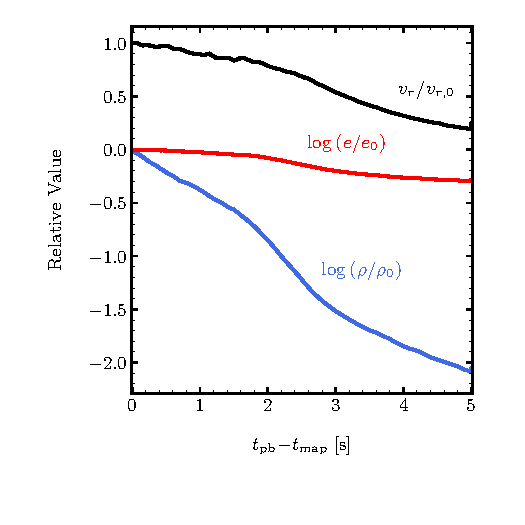
\includegraphics[width=0.50\textwidth,trim=0.2cm 1.2cm 0.2cm 0.2cm,clip]{./pic/wind_paper.pdf}
 \caption{\textbf{Time-dependent behavior of neutrino wind density $\rho$, radial velocity $v_{\mathrm{r}}$ and the total energy density $e$, normalized to their initial values at $t_{\mathrm{map}}\mathord{=}1.44\,\s$, which defines the start of the long-time simulation of the $z9.6$. The data are extracted from a 1D simulation of the explosion of the $9.6\,\solm$ progenitor with \vertexprom \citep{Mirizzi2016}, evaluated at a radius of 600 km.} }
\end{figure}% END FIGURE WIND


\section{Evolution during the first second}
\label{sec:Evolution during the first second}
\subsection{Shock propagation, energetics and neutron star properties}
In the following we provide a short overview of the post-bounce phase. The reader is referred to \cite{Melson2015a} and \cite{Melson2019} for a detailed analysis of the post-bounce phase of the iron-core progenitors. Generic features of the explosion of ECSNe are given in \cite{Kitaura2006,Janka2008,Gessner2018}. Since our results closely resemble these previous findings, we \textbf{summarize} the most important features in the following.
In Figure~\ref{fig:eexp all} we show the evolution of the angle-averaged forward shock and the diagnostic explosion energy of our three-dimensional simulations during the post-bounce phase. 
The angle-averaged supernova shock is calculated as
\begin{equation}
    \langle R_{\mathrm{sh}} \rangle =  \frac{1}{4\pi}\int R_{\mathrm{sh}}(\theta,\phi)\ud \Omega,
    \label{equ:avg rsh}
\end{equation}
where $\ud \Omega\mathord{=}\sin{\theta}\ud\theta\ud\phi$.
The diagnostic explosion energy at any time is given by an integral of total (i.e. kinetic plus internal plus gravitational) specific postshock binding energy, defined as $e_{\text{b}} = e_{\mathrm{int}} + e_{\mathrm{kin}} + \Phi_{\text{g}}$, over volume elements where it has a positive value 
\begin{equation}
    \mathrm{E}_{\mathrm{exp}} = \int_{M} e_{\mathrm{b}} \, \mathrm{dm'},\quad e_{\mathrm{b}} > 0.
    \label{equ:ene exp}
\end{equation}

The sharp drop in density outside the ONeMg-core of model $e8.8$ leads to an early and strong drop in the accretion rate and hence ram pressure at the shock.
Consequently, the forward shock expands rapidly and reaches the core/envelope boundary ($R_{\mathrm{He/H}}\,\mathord{=}\,1210\,\text{km}$), at $0.18\,\s$ after core bounce.
This is in sharp contrast to the typical core-collapse supernova, where the high ram pressure stalls the shock expansion significantly for several $100\,\text{ms}$. The explosion energy starts rising steeply as soon as the forward shock leaves the ONeMg core.

\begin{figure*}
 \centering
 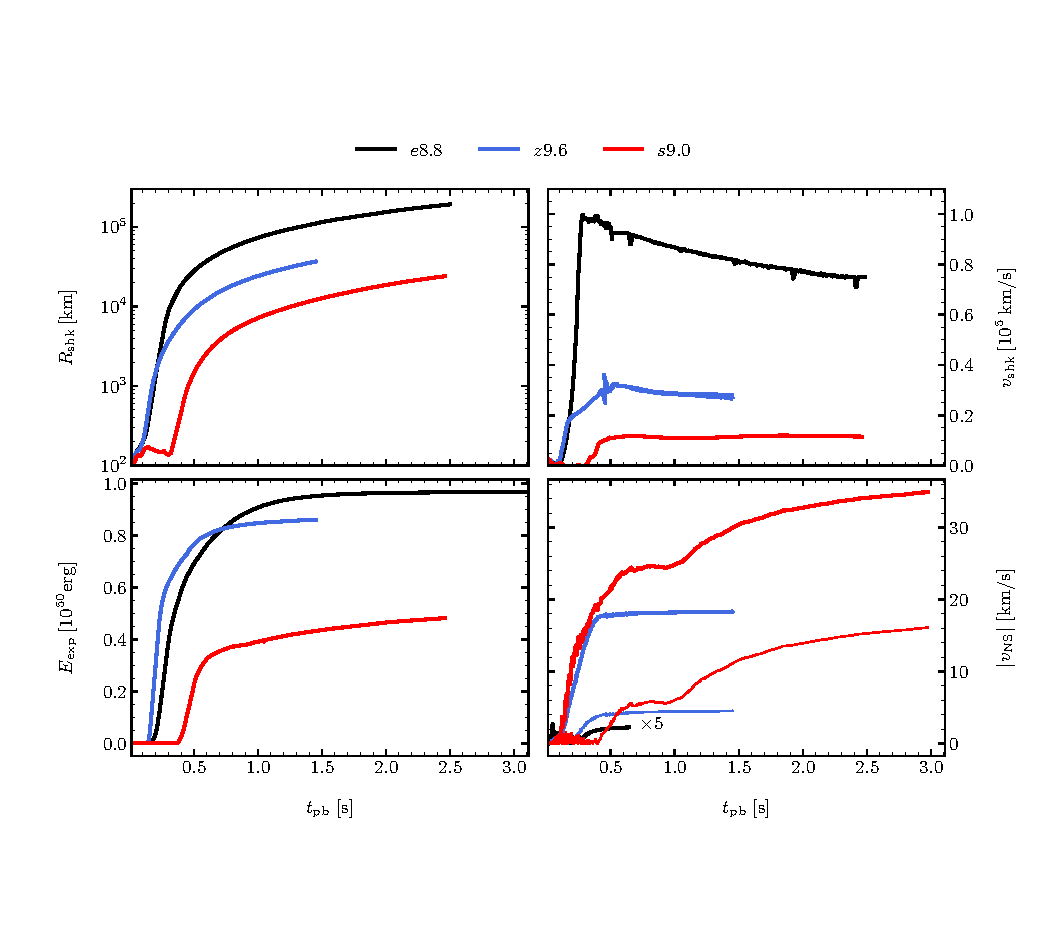
\includegraphics[width=\textwidth,trim=0.1cm 2.1cm 0cm 2.3cm,clip]{./pic/eexp_shk_kick_all_paper.pdf}
 \caption{Shock radius (upper left panel), shock velocity (upper right panel) and diagnostic explosion energy (lower left panel) versus post-bounce time for all of our 3D models. We also show the total PNS kick velocities (thick lines) and hydrodynamic induced PNS kick velocities (thin lines) in the lower right panel. \textbf{The difference is associated with the PNS kicks caused by asymmetric neutrino emission due to the LESA phenomenon (see text for details). For the iron-core progenitors we can track only hydrodynamic contributions to the kick as soon as the transport module of \vertexprom is switched off, while for the ONeMg case our simplified neutrino treatment with the excised core of the PNS does not allow us to monitor the LESA induced kick.}The kick of model $e8.8$ is scaled by a factor of 5 for better visibility. }
\label{fig:eexp all}
\end{figure*}

The acceleration of the shock at the core/envelope boundary is followed by a huge deceleration at the lower boundary of the H-envelope (see upper right panel of Figure~\ref{fig:eexp all}). This is caused by a sudden change of the density gradient at the core/envelope transition.  
Consequently, strong pressure waves are sent upstream into the ejecta, compressing and decelerating the neutrino-heated material.

\begin{table*}
\caption{Overview of PNS properties of our multi-dimensional models at $t_{\mathrm{map}}$.}
\label{tab:neutron star}
\begin{tabular}{cccccccccc||ccc}
    \hline 
            & $t_{\mathrm{map}}$ & 
            $v_{\mathrm{NS,tot}}$ & 
            $v_{\mathrm{NS}}^{\mathrm{hyd}}$ & 
            $v_{\mathrm{NS}}^{\nu}$ &
            $J_{\mathrm{NS}}$    & 
            $\alpha_{\mathrm{ej}}$&
            $\alpha_{\mathrm{ej}}^{\nu}$&
            $M_{\mathrm{b}}$ &
            \rns &
            $M_{\mathrm{fin}}$ &
            $M_{\mathrm{g}}$ &
            $P_{\mathrm{NS}}$ 
            \\
    Model &
    [s]   &
    [km/s] &
    [km/s] &
    [km/s] &
    $[10^{45}\, \mathrm{cm^2 g/s}]$ &
    [\%]              &  
    [\%]              &  
    [\solm]        &
    [km] &
    [\solm]         &
    [\solm]    &
    [s]     \\
    
    \hline
    % model                    tmap    vtot    vhy   vneut      Jns    alhy   alnu    mns        rns      mfin     mfing    pns   
    $e8.8_{3}^{\mathrm{2D}}$ & 2.515 & 1.55  & 1.55  & -     & 1.80  & 1.154 &  -     & 1.323 &  49.85 &  1.334 &  1.216 &  0.65 \\
    $e8.8_{6}^{\mathrm{2D}}$ & 2.515 & 0.94  & 0.94  & -     & 2.70  & 0.041 &  -     & 1.316 &  50.22 &  1.327 &  1.210 &  0.43 \\
    $e8.8_{10}^{\mathrm{2D}}$& 2.515 & 0.13  & 0.13  & -     & 4.19  & 0.004 &  -     & 1.308 &  50.57 &  1.319 &  1.203 &  0.27 \\
    $e8.8_{15}^{\mathrm{2D}}$& 2.515 & 0.59  & 0.59  & -     & 1.66  & 0.011 &  -     & 1.299 &  50.86 &  1.309 &  1.195 &  0.69 \\
    $e8.8_{10}^{\mathrm{3D}}$& 0.470 & 0.44  & 0.44  & -     & 0.69  & 0.004 &  -     & 1.307 &  50.57 &  1.326 &  1.209 &  1.68  \\
    $z9.6$                   & 3.140 & 19.28 & 10.16 & 24.89 & 1.73  & 4.623 & 1.354  & 1.340 &  20.98 &  1.340 &  1.221 &  0.68 \\
    $s9.0$                   & 1.440 & 36.32 & 29.65 & 26.22 & 7.60  & 10.02 & 1.178  & 1.299 &  19.58 &  1.299 &  1.128 &  0.15  \\
    \hline
\end{tabular}
\flushleft
\textit{Notes}: \textbf{All values are given at the end of our explosion simulation ($t_{\mathrm{map}}$). $v_{\mathrm{NS}}^{\mathrm{tot}}$ is the total NS kick resulting from the hydrodynamic ($v_{\mathrm{NS}}^{\mathrm{hyd}}$) plus the neutrino-induced ($v_{\mathrm{NS}}^{\mathrm{\nu}}$) contribution. $J_{\mathrm{NS}}$ is the total angular momentum transported to the PNS through a radius of 100 km \COM{I include inward and outward flux of angular-momentum}. $\alpha_{\mathrm{ej}}$ and $\alpha_{\mathrm{ej}}^{\nu}$ are the hydrodynamic and neutrino anisotropy-parameter, respectively (see Appendix~\ref{Appendix:neutron star}). For the iron-core progenitors we average $\alpha_{\mathrm{ej}}^{\nu}$ over the time the emission dipole is the largest until the end of the simulation. $M_{\mathrm{b}}$ is the baryonic PNS mass. $P_{\mathrm{NS}}$ is the PNS spin period at the end of our post-bounce simulations assuming a final PNS radius $R_{\mathrm{NS}}$ of 12 km, angular momentum conservation and a gravitational mass of $M_{\mathrm{g}}$. $M_{\mathrm{fin}}$ (see also Table~\ref{tab:long term boundaries}) is the mass contained within the excised region from which we calculate and gravitational mass $M_{\mathrm{g}}$ of the PNS. }
\end{table*}

%z9.6
The ECSNe-like structure of model $z9.6$ is reflected in the evolution of the forward shock and growth of the diagnostic explosion energy. Shock radii remain almost perfectly spherical \textbf{in both the $e8.8$ and $z9.6$}. Acceleration of the forward shock outside the iron-core, however, is weaker in the $z9.6$ model than in model $e8.8$, due to the more gradual change in the density profile. Explosion energies also start to rise early and saturate just after $\tpb\mathord{\sim}1\,\s$.

%s9.0
In contrast to the $z9.6$ and $e8.8$ models, the $s9.0$ is lacking the very steep density gradient outside the Fe-core, as can be seen in Figure~\ref{fig:prog_tem_rho_ye_rhor}
The shock can expand initially up to $180\,\km$ at $\tpb\mathord{\sim}130\,\ms$ but then \textbf{enters a phase of recession}. The \textbf{arrival} of the Si/O interface at the shock and \textbf{the decreasing mass-accretion rate} within the oxygen shell, eventually lead to shock expansion at $\mathord{\sim}0.3\,\s$ after bounce. Shock expansion is aided by strong convection behind the shock front. Similar to the results presented in \cite{Glas2019}, who used the same progenitor, the model remains convection-dominated and does not indicate any signs of the standing-accretion shock instability (SASI) \citep{Blondin2003,Foglizzo2007}.
However, although SASI does not develop in the simulation, the forward shock experiences \textbf{large-scale deformations with a dipole amplitude of $10\mathord{-}10\%$ (compared to the angle-averaged shock radius)}. These deformations are driven by large scale plumes that form in the postshock layer. 
Contrary to the ECSN-like models, strong non-radial motions persist \textbf{around the PNS} over several seconds after bounce. Continuous mass accretion on the PNS through small funnels delay the emergence of the spherical neutrino-driven wind, which is why we needed to continue the simulations over three seconds after bounce.

%% FIGURE Initial Ni+X all Progenitors
\begin{figure*}
 \centering
 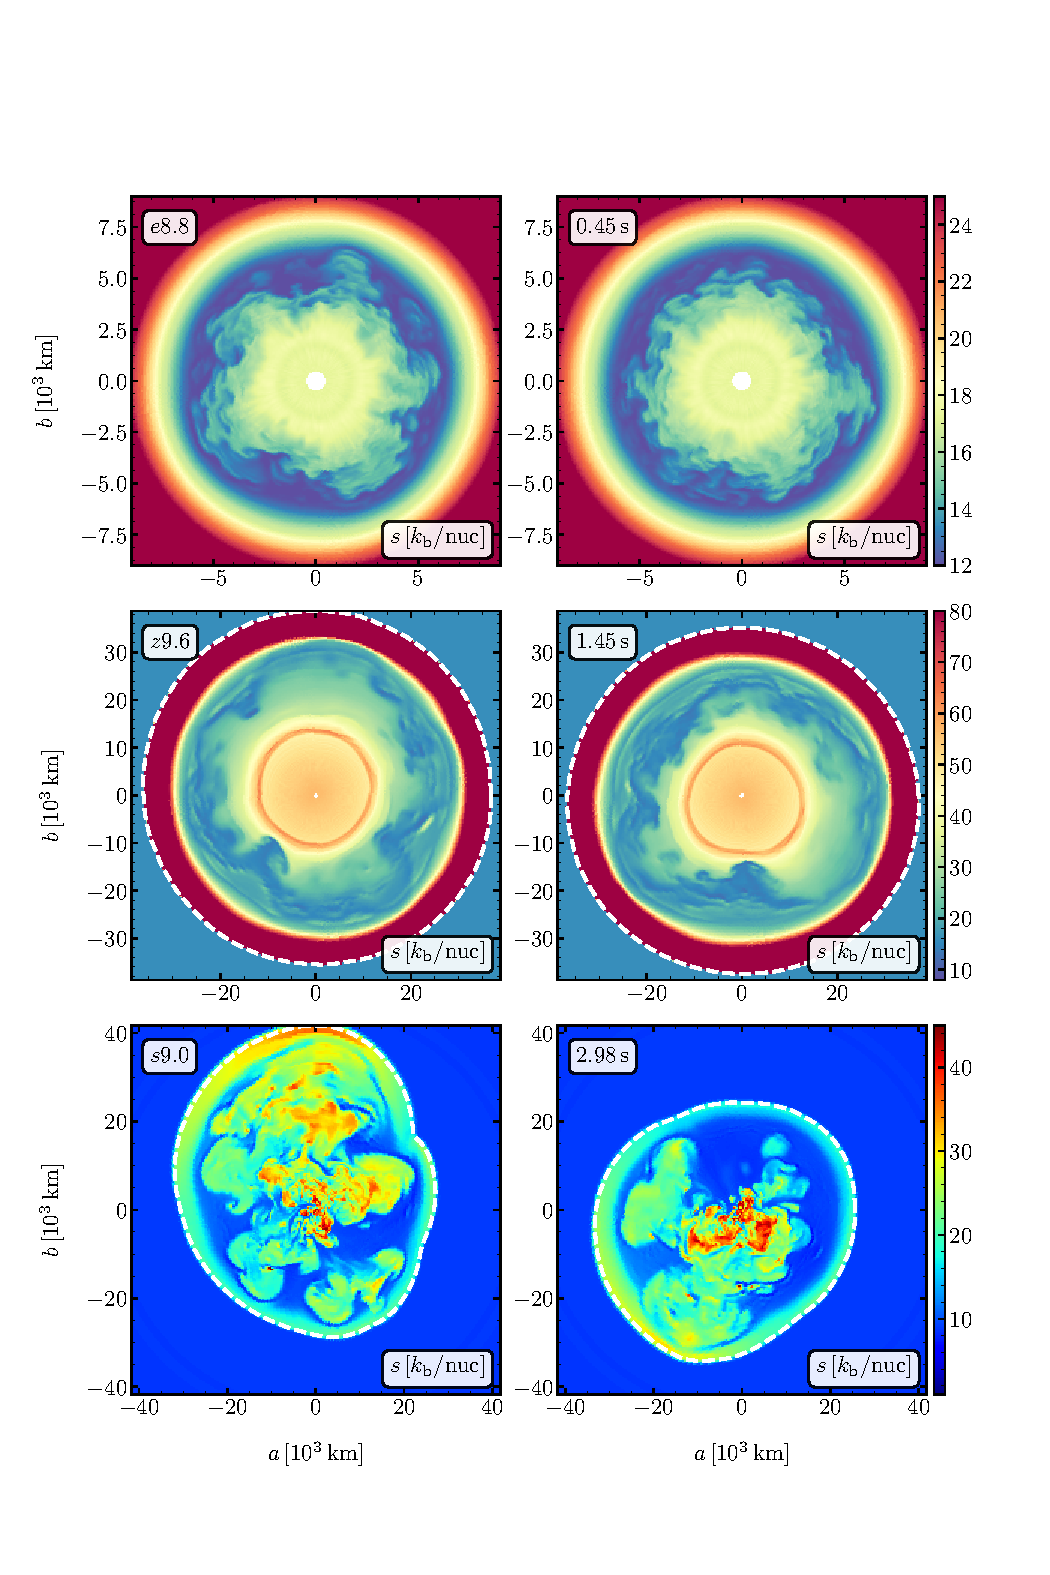
\includegraphics[width=0.95\textwidth,trim=0cm 1.8cm 0cm 3cm,clip]{pic/all_3d_sto_slices_time_0.pdf}
 \caption{Planar cuts of our 3D models showing the entropy color-coded at $t_{\mathrm{map}}$. The left panels display cuts which are aligned such that the point of largest shock deformation is included in the plane. Therefore the coordinate directions of the plots have no association with the computational-grid coordinates. The right panels include the smallest shock expansion in the plane. Note the largely spherical morphology of model $e8.8$ and the deformed ejecta morphology of model $s9.0$. For better visibility of the small scale structures of model $s9.0$ we chose a different color representation in this case.}
 \label{fig:slices first mapping}
\end{figure*}
In order to compare the final state of the post-bounce simulations of our model set, we \textbf{present} in Figure~\ref{fig:slices first mapping} planar cuts showing the entropy at the times ($t_{\mathrm{map}}$) we start our long-term simulation. The left panels are chosen such that they include the plane of the largest shock deformation. The right panels include the plane of the smallest shock deformation.
Note the \textbf{basically spherical shape of the shock and the mild postshock asymmetries} in both the $e8.8$ and $z9.6$ models.
In strong contrast to the ECSNe-like models, the $s9.0$ shows a clear dipolar shock deformation and ejecta morphology. 

The asymmetries that develop during the explosion also affect the kick of the PNS.
In Table~\ref{tab:neutron star} we provide properties of the PNS resulting from our post-bounce simulations\footnote{We refer the reader to Appendix~\ref{sec:Neutron Star Properties} for the equations involved in the analysis presented in Table~\ref{tab:neutron star}.}. We list the PNS kick velocity ($v_{\mathrm{NS}}$), anisotropy parameter ($\alpha_{\mathrm{ej}}$), angular momentum ($J_{\mathrm{NS}}$) and spin period ($P_{\mathrm{NS}}$) along with the PNS radii (\rns) and baryonic PNS masses ($M_{\mathrm{b}}$) at the point in time we terminate the post-bounce simulations. The PNS radius $\rns$ is defined as the angle-dependent radius where the density drops below $10^{11}\,\mathrm{g/cm^3}$. The PNS mass $M_{\mathrm{b}}$ is the mass contained within $\rns$. $M_{\mathrm{fin}}$ is the mass contained within our inner boundary for the long-term simulations (see Table~\ref{tab:long term boundaries}) and $M_{\mathrm{g}}$ the respective gravitational mass.
The acceleration of the PNS is caused by two different mechanisms.
\textbf{Firstly, aspherical ejection of matter leads to a gravitational ``tug'' which accelerates the PNS in the opposite hemisphere of maximum shock expansion and fastest ejecta. Second, anisotropic neutrino emission, due to the ``lepton-emission self-sustained asymmetry'' (LESA) \citep{Tamborra2014}, can accelerate the PNS opposite to the direction of the largest total neutrino-energy flux.
The almost spherical explosions of the ECSNe-like progenitors yield low hydrodynamic kick velocities. Anisotropic neutrino emission does not play a role in the simulation of model $e8.8$, because of the spherical treatment of the central region. The contribution of anisotropic neutrino emission in models $z9.6$ and $s9.0$, however, even exceeds the contribution due to aspherical ejection of matter. LESA manifests itself in a dominant and stable $\ell\mathord{=}1$ mode of the lepton-number emission and a corresponding energy-emission dipole of several percent amplitude compared to the monopole (see \citealt{Tamborra2014}). LESA is observed in both simulations conducted with \vertexprom. }

We show in Figure~\ref{fig:sto ye s9 z9 kick} planar slices of the electron fraction (left panels) and entropy (right panels) of the iron-core progenitors. The black, blue and green arrows indicate the total, hydrodynamic and neutrino-induced directions of the PNS kick. In case of the $z9.6$ the hydrodynamic and neutrino-induced kicks are clearly aligned. This stems from the feedback mechanism which is associated with LESA. Increased heating in the direction opposite to the LESA dipole pushes the supernova shock to larger radii. The induced asymmetry of the postshock ejecta feeds back into the hydrodynamic acceleration of the PNS. Due to the weak convection in the $z9.6$ model, the emission asymmetry is the dominant contribution to drive the PNS kick. 
Where the gravitational tug can only account for  $v_{\mathrm{NS}}^{\mathrm{hyd}}\mathord{\sim}10\,\kms$, the asymmetric emission of neutrinos enables a kick velocity up to $v_{\mathrm{NS}}^{\mathrm{\nu}}\mathord{\sim}25\,\kms$. The total kick sums up to $v_{\mathrm{NS}}^{\mathrm{tot}}\mathord{=}19\,\kms$.
The alignment of the neutrino-induced and hydrodynamic kick is less clear in the $s9.0$. Although the neutrino emission is the largest contribution to the total PNS kick during the first 500 ms, strong non-radial motions in the post-shock region impose their asymmetries onto the forward shock. 
The hydrodynamically induced dipolar shock expansion of the $s9.0$ and contributions from the LESA dipole yield a total acceleration of the PNS to $v_{\mathrm{NS}}\mathrm{\sim}36.32\,\kms$.
\COM{Question: What effect has the early disabling of neutrino transport? Neutrino-induced kick has not saturated. }

\begin{figure*}
 \centering
 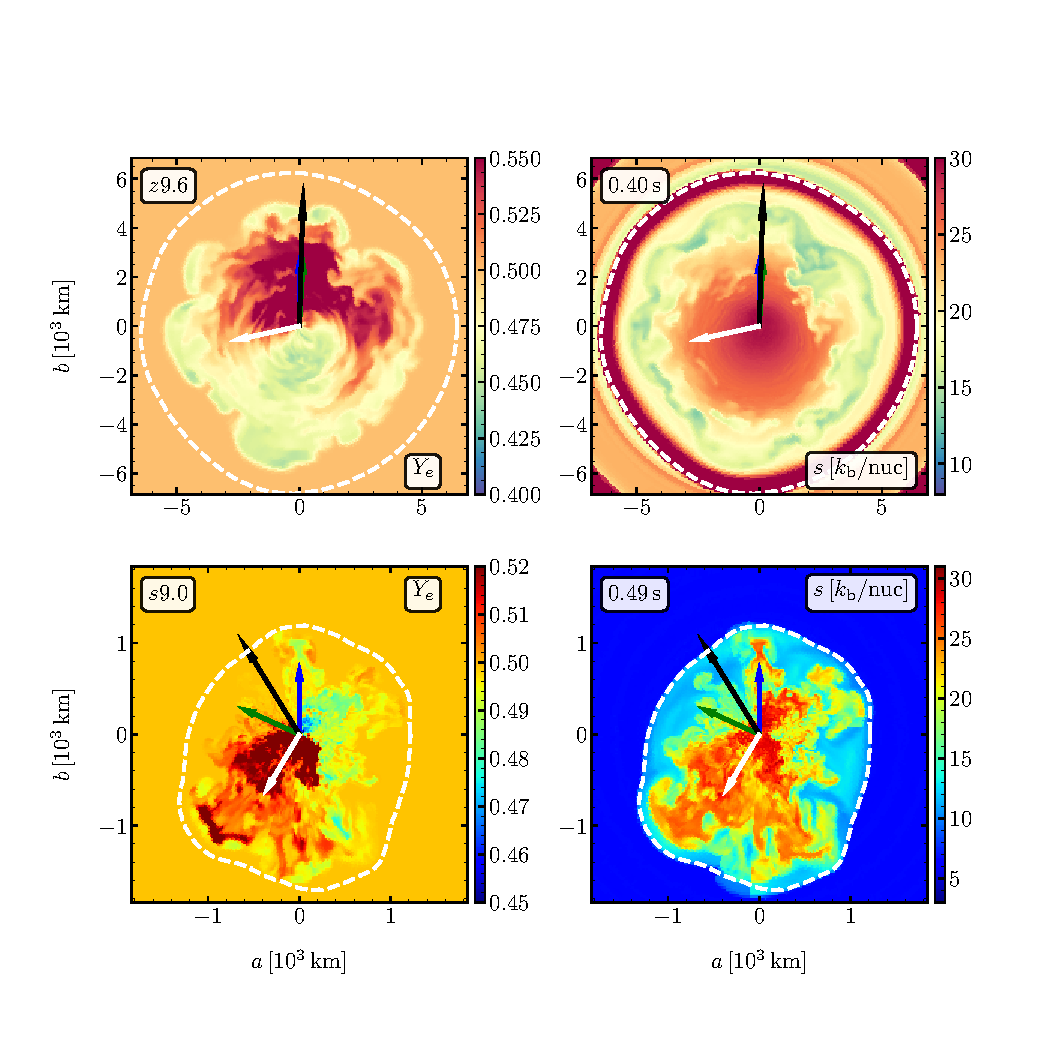
\includegraphics[width=\textwidth,trim=0cm 1.3cm 0cm 2cm,clip]{pic/z9_s9_3d_ye_sto_kick_slices.pdf}
 \caption{\textbf{Planar slices of the electron fraction $Y_{e}$ (left panels) and entropy (right panels) of the $z9.6$ and $s9.0$. The planes are chosen such that the hydrodynamic kick is pointing to the north and are not aligned with the global coordinate system. The arrows indicate the direction of the total kick (black), the hydrodynamic and neutrino kick (blue and green) and the direction of the LESA dipole (white).}}
 \label{fig:sto ye s9 z9 kick}
\end{figure*}

\subsection{Extent of mixing at shock revival}
\label{sec:Extent of mixing at shock revival}

In order to access the strength of mixing during the first second in our 3D models, we present in Figure~\ref{fig:mdp first mapping} fractions of the total mass of selected elements as a function of velocity (top panels) and mass coordinate (lower panels). 
For sampling the velocity space, we chose 50 bins between the maximal and minimal velocities within the considered region. We use 30 bins to sample the distribution in mass coordinate.

The spherical explosion of the $e8.8$ manifests itself also in the distribution of elements over mass and velocity space, where the initial shell-like structure of the progenitor is maintained.
The thin carbon-shell of the progenitor is traveling with $\sim 40\mathord{-}50\,\mathrm{1000\,km/s}$ in front of the outer mass-shells of the former ONeMg-core, which travel at $\sim 35\,\mathrm{1000\,km/s}$. Most of the newly synthesized iron-group and $\alpha$ nuclei travel at velocities below $\sim 35\,\mathrm{1000\,km/s}$.
Early deceleration of the shock also confines the neutrino-heated ejecta within $M(r)\mathord{\le 1.33}\,\solm$.

%z9.6
Slightly more violent convection in the $z9.6$ model lead to more efficient mixing in mass and velocity space (see left panels of Figure~\ref{fig:mdp first mapping}). Some neutrino-heated material could already be mixed into the carbon and oxygen shells that travels at $20\times 10^3\,\kms$. The bulk of the metal-rich ejecta still travels with slower velocities, however. 
Similar to the $e8.8$, the deceleration of the forward shock at the Si/O and CO/He interfaces in the $z9.6$ also compressed some of the matter into a dense shell. 
%s9.0 
The $s9.0$ model, again, differs strongly from the ECSN-like models. 
Long-lasting convection completely erased the initial onion-like shell structure of the progenitor. Elements are homogenously mixed over mass and velocity coordinate (see middle panels of Figure~\ref{fig:mdp first mapping}).
The fastest neutrino-heated ejecta are caused by a large high entropy plume inducing a bipolar perturbation on the shockwave, which can be see in Figure~\ref{fig:slices first mapping}.

%% FIGURE Mass Distribution all Progenitors
\begin{figure*}
 \centering
 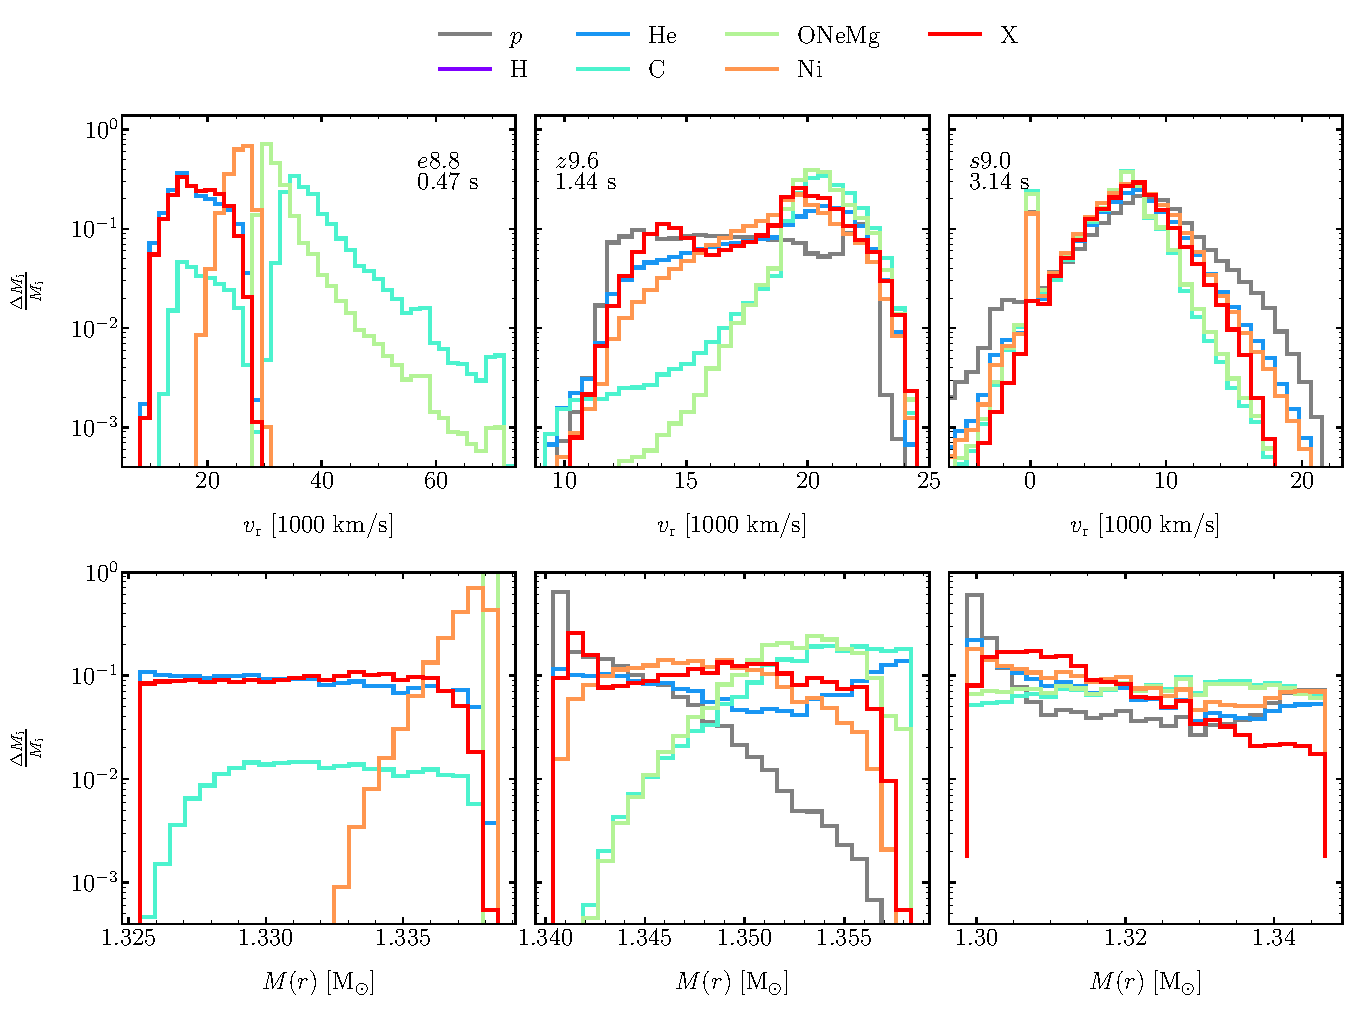
\includegraphics[width=\textwidth,trim=1.1cm 0.6cm 1cm 0cm,clip]{pic/z96_s9_e8_3d_massDis_mvr_and_masstime_0_paper.pdf}
 \caption{Binned distribution of elements as a function of radial velocity (top panels) and enclosed mass (bottom panels) for all our 3D models at $t_{\mathrm{map}}$ (see Table~\ref{tab:long term boundaries}). We use 50 bins in velocity space and 30 bins in mass coordinate. See text for discussion.}
 \label{fig:mdp first mapping}
\end{figure*}

\begin{table*}
    \centering
    \begin{tabular}{lcc}
        &
        \multicolumn{2}{c}{$e8.8$} \\
         Species &
         $M_{\mathrm{init}}$ &
         $M_{\mathrm{fin}}$ \\
                 &
         $[M_{\mathrm{\odot}}]$ &
         $[M_{\mathrm{\odot}}]$ \\
         \hline 
            p               & 2.7                & 2.895e+00 \\
            He4             & 1.8                & 1.745e+00 \\
            C12             & $2.2\times10^{-2}$ & 2.196e-02 \\
            O16+Ne20+Mg24   & $5.0\times10^{-2}$ & 4.972e-02 \\
            Ni56+Fe56       & $3.4\times10^{-3}$ & 2.653e-03 \\
            X56             & $1.3\times10^{-2}$ & 1.301e-02 \\
            rest            & $5.6\times10^{-2}$ & 5.593e-02 \\
            \hline \\
            X Sum           & 4.641e+00 & 4.583e+00 \\
            + pm            & 5.959e+00 & 5.901e+00   
    \end{tabular}
    \caption{Caption}
    \label{tab:my_label}
\end{table*}

\section{Evolution until Shock-Breakout}
\label{sec:Evolution until Shock-Breakout}
\subsection{Linear stability analysis}
\label{sec:Linear stability analysis}
As already mentioned, the velocity of the forward shock depends on the progenitor structure, in particular the $\rho r^3$-profile. According to \cite{Sedov1961} one expects a \textbf{increase/decrease} in the shock velocity when the gradient of the $\rho r^3$-profile is positive/negative. 
\textbf{This acceleration and deceleration leads to crossing of the density and pressure gradients in the postshock region, or stated otherwise, the gradients of the pressure and density have opposite signs.} Thus, perturbations in the matter become unstable to the Rayleigh-Taylor instability \citep{Rayleigh1882,Chevalier1978}. As the $\rho r^3 $-profiles, and hence the shock speed, vary significantly between the progenitors, growth of Rayleigh-Taylor instabilities will affect the long-term evolution of our models in different ways.

In order to aid us with the interpretation of our three-dimensional simulations, we appeal to 1D simulations which are started from angle-averaged initial states of the 3D data. The numerical and physical setup for the spherically symmetric simulations remains unchanged. 
They can teach us about the behavior of the shock, while it propagates through the envelope. 
Additionally, we compute the linear RT growth rates $\sigma_{\mathrm{RT}}$ of small initial perturbations by tracking Lagrangian mass coordinates in our 1D simulations, following \cite{Mueller1991}. 
In the incompressible case the growth rate is given by
\begin{equation}
  \label{equ:growth rates incmp}
  \sigma_{\mathrm{RT,incmp}} = \sqrt{- \frac{p}{\rho}\frac{\partial \ln p}{\partial r}\frac{\partial \ln \rho}{\partial r}},
\end{equation}
where $p$ and $\rho$ are the pressure and density. In the compressible case the growth rate becomes
\begin{equation}
  \sigma_{\mathrm{RT, cmp}} = \frac{c_{s}}{\gamma}\sqrt{\Big(\frac{\ln p}{\partial r}\Big)^ 2 - \gamma \frac{\partial \ln p}{\partial r}\frac{\partial \ln \rho}{\partial r}},
  \label{equ:growth rates cmp}
\end{equation}
where $c_{\mathrm{s}}$ is the speed of sound and $\gamma$ the adiabatic index. Equation~\ref{equ:growth rates cmp} is less restrictive than its incompressible counterpart\footnote{Note that we are interested in the locations of maximal growth but not in the actual values. Calculating the growth factors from multidimensional models using angle averaged values gives similar overall structure but lower amplitudes \citep{Mueller2018}.}. 
For the time-dependent amplification factor we integrate Equation~\ref{equ:growth rates cmp} according to
\begin{equation}
  \Sigma_{\rm RT}(t) = \frac{\xi}{\xi_0}(t) = \exp \left(\int_0^t \sigma_{RT} (t') dt' \right).\label{equ:growth rates int}
\end{equation}
This analysis enables us to estimate the time and locations in mass coordinate, where the fluid becomes unstable to the RTi and thus helps us to understand the origin of outward/inward mixing of \textbf{different layers with their chemical elements}.

We show in Figure~\ref{fig:growth rates} the amplification factors in the compressible (magenta lines) and incompressible (red lines) cases for our spherically symmetric simulations. Significant differences between the models are evident.
\begin{figure*}
 \centering
 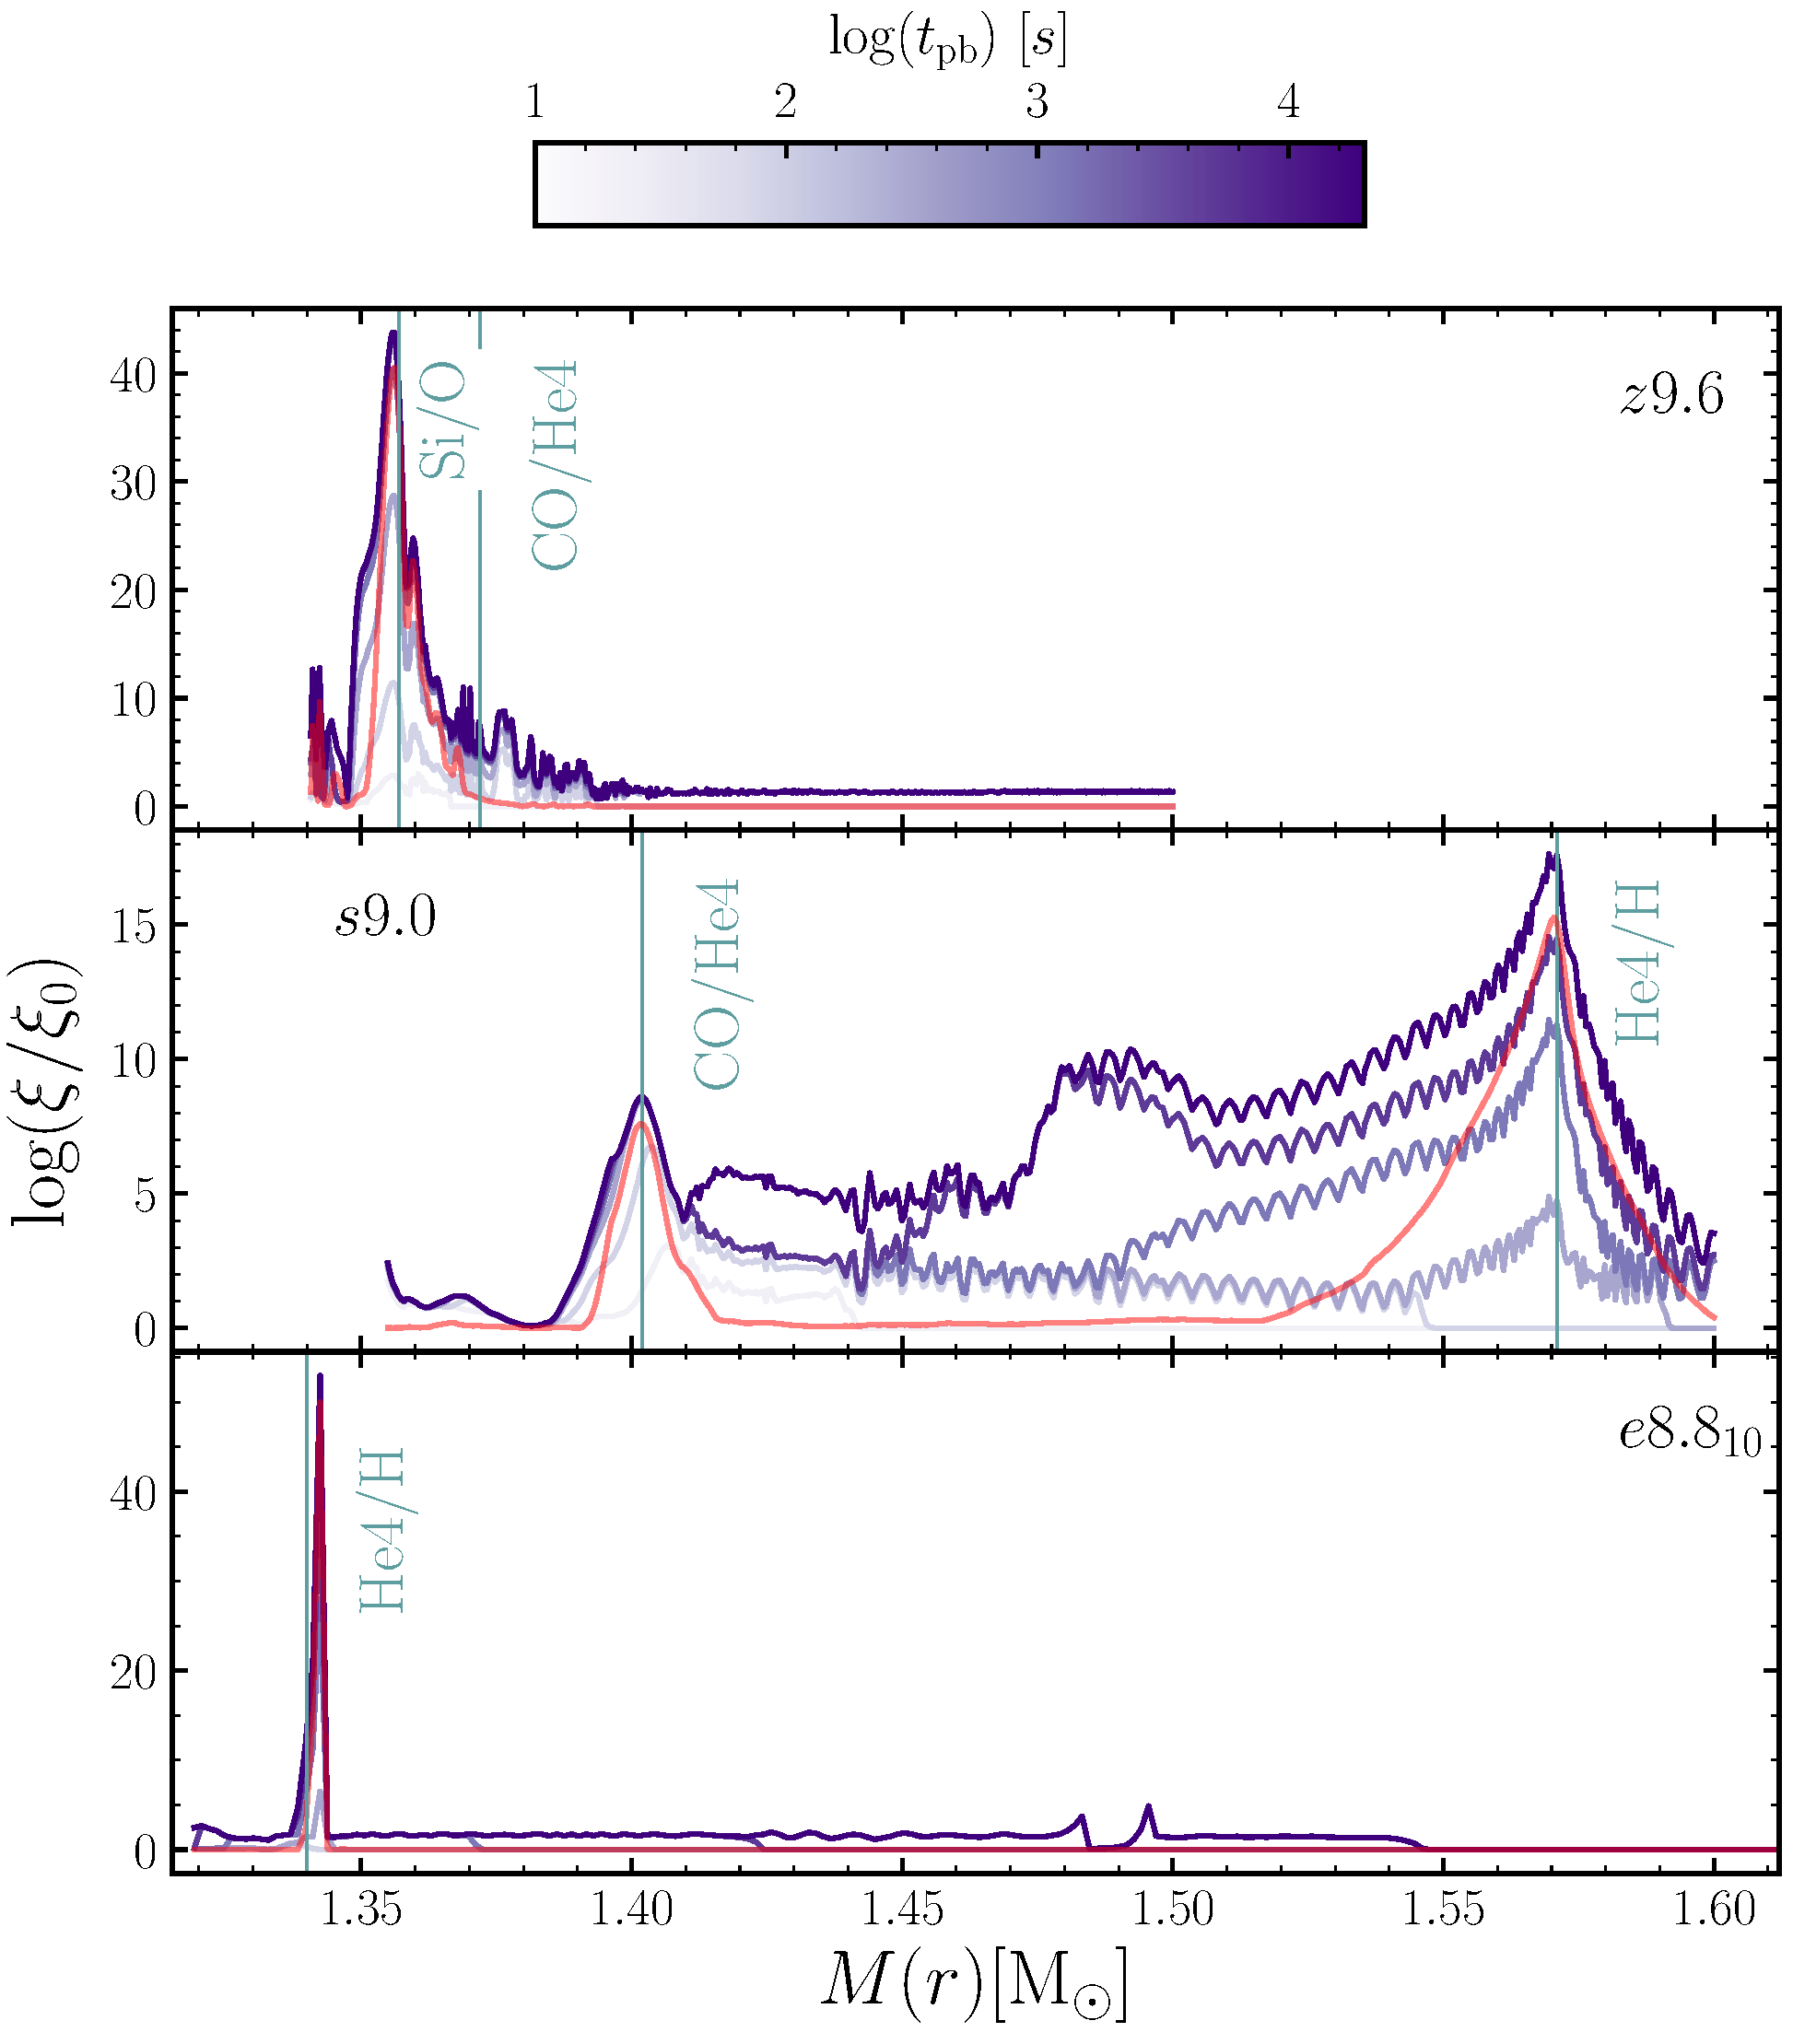
\includegraphics[width=\textwidth]{pic/growth_rates_1d.pdf}
 \caption{Integrated growth rates for all considered models at different times evaluated with Equation~\ref{equ:growth rates int} (magenta lines). Indicated by the blue lines are the respective composition interfaces. The red line denotes the evaluation of the growth rates in the incompressible limit at $t=10^{4}\,\text{s}$. The different progenitor structures have a large impact on the estimated growth as can be seen most prominently by comparing the z9.6 and so s9.0 models. \COM{Match colors to composition Figure ?} }
 \label{fig:growth rates}
\end{figure*}

The right panel of Figure~\ref{fig:growth rates} shows the integrated growth-rate of the $e8.8_{10}$ model.
The extreme deceleration of the forward shock when moving into the hydrogen envelope induces very high growth factors at $M(r)\mathord{=}1.34\,\mathrm{M_{\odot}}$.

The ECSN-like structure of model $z9.6$ is reflected in the amplification factors.
Strong deceleration of the forward shock at the core/hydrogen interface created the necessary condition for the RTi to grow. As can be seen in Figure~\ref{fig:growth rates}, amplification factors at $\mathord{\sim}1.36\,\solm$ between the C/He and He/H interfaces of model $z9.6$ (see Table~\ref{tab:progenitors}) almost reach values as high as observed in the ECSN case. Interestingly, no growth is expected at the He/H interface, which stems from the very small step in the $\rho r^3$ profile at this interface (see Figure~\ref{fig:prog_tem_rho_ye_rhor}).
Model $s9.0$ shows striking differences to the models described above. 
Due to its more shallow $\rho r^3$-profile in the core region and the consequently weaker episodes of de- and acceleration, the peak amplitudes of the growth factors are smaller. They are, however, of the same strength as in the more massive models investigated by \cite{Wongwathanarat2015}. 
Similar to the red supergiants presented in \citet{Wongwathanarat2015}, the strongest contribution arises from the He/H interface followed by the CO/He interface where amplification factors  reach values of $8-16$, respectively. 
A characteristic not mentioned by \cite{Wongwathanarat2015} is the vast difference in the compressible versus incompressible evaluation of the growth factors. In the compressible case a large contribution between both interfaces is visible.
\textbf{This, however, is not of immediate relevance, because the peaks of the growth factors at the CO/He and He/H interfaces, which we captured in the incompressible case, dominate by far. At the times the compressible analysis predicts growth factors of significance ($\tpb\mathord{\sim}10^{3\mathord{-}4}$) between both interfaces, the RTi will long have reached the non-linear stage, thus deprecating the value of a linear stability analysis.}

%% NEW STUFF
\subsection{Propagation of forward shock and neutrino-heated ejecta }

We show in Figure~\ref{fig:radii all times} the angle-averaged shock radii and shock velocities of our 3D simulations.
When the 3D simulation of model $e8.8$ \textbf{is continued from the neutrino-powered initial phase and mapped to the long-term evolution at $\tpb=0.470$, the forward shock has long passed the He/H interface and is traveling through the H-envelope (see lower left panel of Figure~\ref{fig:radii all times})}. It had left the ONeMg core with some $7.5\times 10^{3}\,\kms$ and is continuously decelerated due to the monotonic increase of the $\rho r^3$-profile.
Interestingly, the neutrino-heated ejecta, which can be traced by the \nickel+\tracer=0.1\% iso-surface, catch up with the forward shock at $\tpb\mathord{\sim}130\,\s$ and push it to slightly higher velocities. 
The early and strong deceleration of the forward shock in the hydrogen envelope of the ECSN progenitor lead to an early formation of a dense shell in the post shock region. At the bottom of this dense shell or ``wall'' \citep{Kifonidis2006} a reverse shock forms. To illustrate this we show in Figure~\ref{fig:density profiles all times} radial profiles of the density of our 1D long-term simulations\footnote{We show the results of the 1D long-term simulations because the formation and propagation of the dense shell and reverse shock is basically independent of the chosen dimensionality but provides an easier ground for our analysis. }. In the left panel of Figure~\ref{fig:density profiles all times} the dense shell is visible as the peak-like feature at $3\times\mathord{\sim}10^{5}\,\mathrm{km}$ in the first profile. 
Continuous deceleration of the forward shock eventually causes the reverse shock to travel back in mass coordinate, starting at  $\tpb\mathord{\approx}\,1\text{h}$. It takes, however, additional $7\,\text{h}$ for the reverse shock to reach the inner boundary of our computational domain. Shock breakout is observed at $\tpb\mathord{\sim}5\,\text{d}$.
%z9.6
The shock trajectory of model $z9.6$ is quite similar to the trajectory observed in model $e8.8$. However, the initial velocity of the forward shock is smaller by a factor of two, which stems from the less steep density gradient at the core/envelope transition. Moreover, the deceleration of the forward shock is less severe (see Figure~\ref{fig:radii all times}) in model $z9.6$. The bulk of the neutrino-heated ejecta are not able to catch up with the forward shock.
The strong deceleration outside of the CO core and the continuous deceleration of the forward shock in the helium shell, cause the formation of a reverse shock fairly early at $\tpb\mathord{\sim} 100\,\s$. Until $\tpb\mathord{\sim}\, 300\,\s$ forward and reverse shock travel with roughly equal velocity through the He core. 
After $300\,\s$ after bounce, the reverse shock begins to fall back until and reaches the inner boundary at $t_{\mathrm{pb}}\sim 1.14\,\text{h}$. This is more than 6 hours earlier than in the $e8.8$ case. We observe shock breakout at $\tpb\mathord{\sim}\, 29\,\mathrm{h})$. \COM{REVERSE SHOCK IN FIGURE}
%s9.0
As expected from the $\rho r^3$-profile of model $s9.0$ the forward shock experiences phases of strong de- and acceleration while passing through this progenitor. In contrast to the ECSNe-like models, the forward shock accelerates shortly before the He/H interface. The subsequent strong deceleration in the hydrogen envelope is the reason for the large growth rates observed at the He/H interface (see Figures~\ref{fig:prog_tem_rho_ye_rhor} and~\ref{fig:radii all times}). 

\begin{figure*}
 \centering
 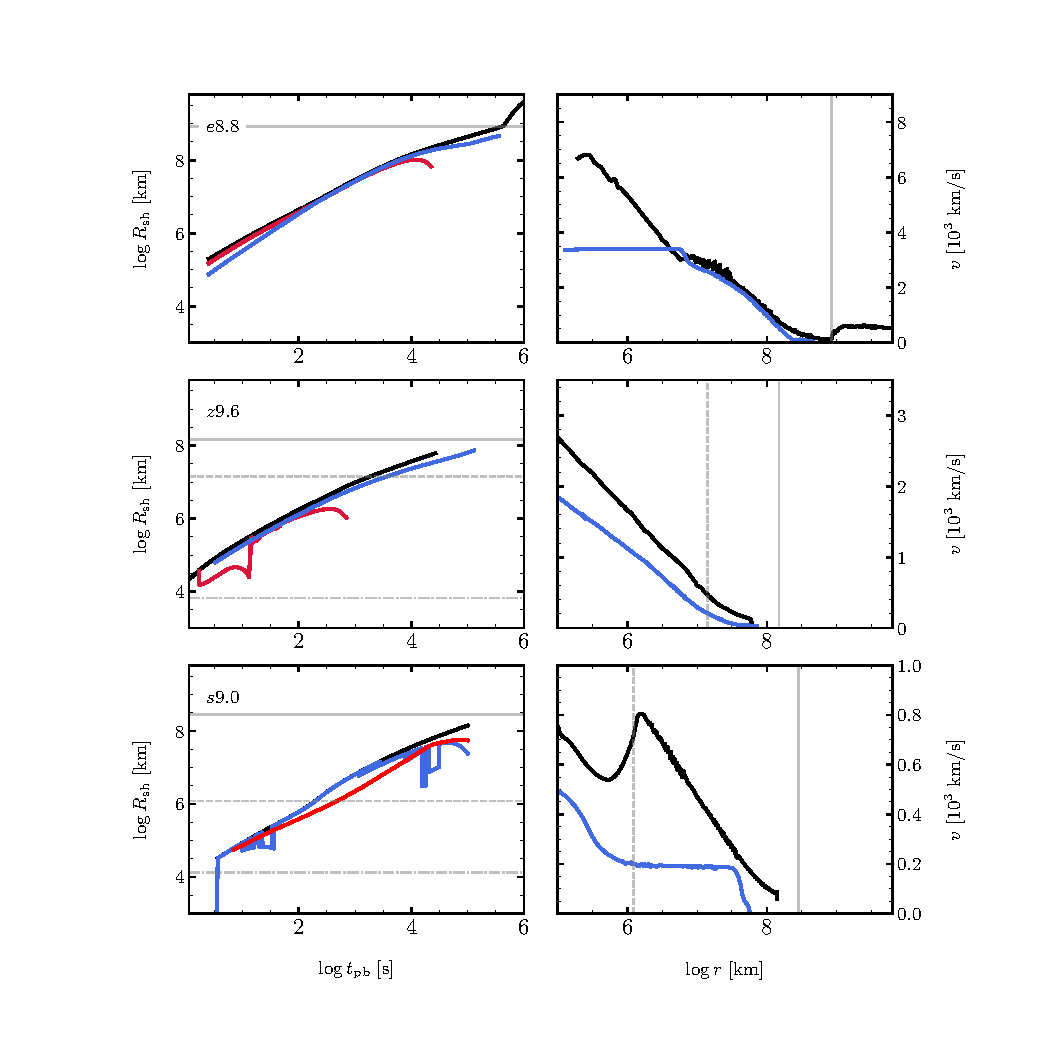
\includegraphics[width=\textwidth, trim=0cm 1.0cm 0cm 1.0cm,clip]{pic/radii_velocity_shock_nickel.pdf}
 \caption{Left Panels: Angle-averaged shock radius (black lines) and averaged radius of the $\nickel+\tracer\mathord{=}0.1\,\%$ surface (blue lines) of our long-term simulations. Right Panels: Shock velocity (black lines) and velocity of the $\nickel+\tracer\mathord{=}0.1\,\%$ surface (blue lines) as a function of radius. The dash-dotted, dashed and dotted lines indicate the CO/He, He/H interfaces and the surface of the progenitor, respectively. \COM{Add reverse shock radii.}}
 \label{fig:radii all times}
\end{figure*}

\begin{figure*}
 \centering
 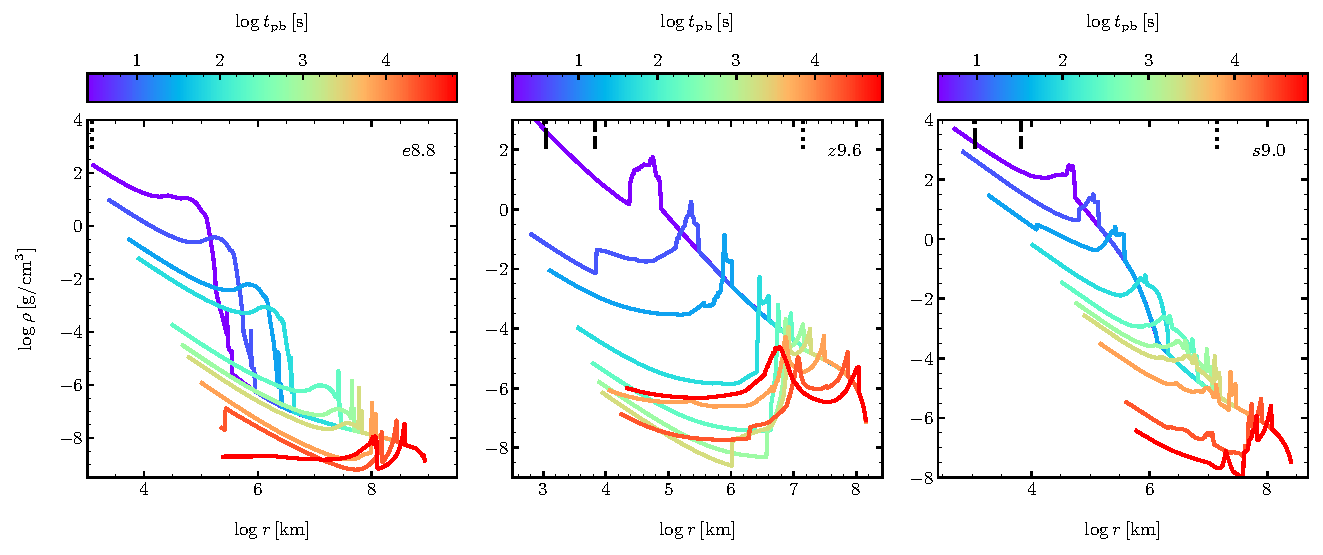
\includegraphics[width=\textwidth, trim=0cm 0.0cm 0cm 0.0cm,clip]{pic/density_profiles_1d_long_term.pdf}
 \caption{Radial profiles of the density of our 1D long-term simulations at representative times. The dashed, dash-dotted and dotted lines represent the outer boundaries of the iron-, CO and He cores. See text for discussion.}
 \label{fig:density profiles all times}
\end{figure*}

\COM{COMMENT ON NICKEL VELOCITIES FOR iron-coreS}

\subsection{Ejecta morphology}
% e8.8
In Figure~\ref{fig:e8 3d 4times} we show planar cuts of the $\nickel\mathord{+}\tracer$ mass fraction of the ECSN model at representative epochs. The forward shock is outside the visible plane. 
Shortly after onset of the explosion of the $e8.8$ model, the neutrino heated high entropy plumes basically freeze in their angular distribution and expand into the low density H-envelope. 

\begin{figure*}% Figure e8.8 rho cuts
 \centering
 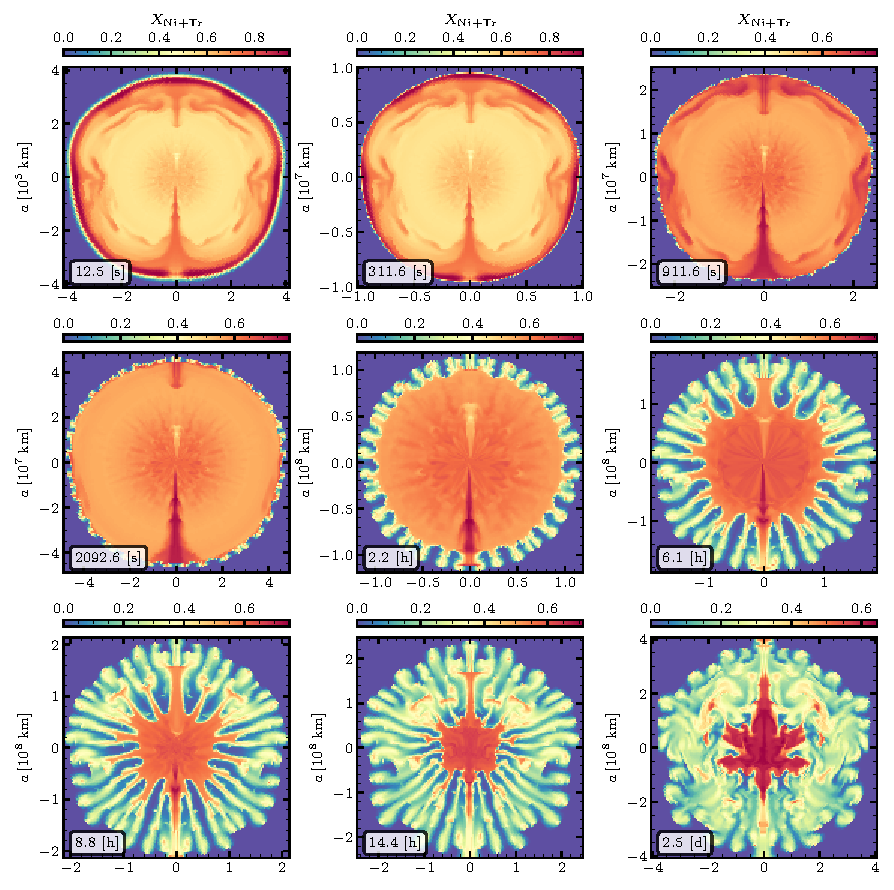
\includegraphics[width=\textwidth,trim=0.2cm 0cm 0cm 0cm,clip]{pic/e8_10_3x3_NiX.pdf} 
 \caption{Planar cuts through the $e8.8_{\mathrm{2D}}$ model at the indicated times showing the \nickel+\tracer mass fraction. Note that the shock radius is outside the shown domain. Until $\tpb\mathord{\sim} 300\,\s$ the initial high entropy plumes expand essentially self-similar. At $\tpb\mathord{\sim} 300\,\s$ the plumes catch up with the dense shell that formed due to the deceleration of the shockwave in the hydrogen envelope and are thereby compressed. The growth of small scale perturbations at the He/H interface leads to some outward mixing of \nickel in small cusps. The cusps grow to considerable size until $\mathord{\sim}14.4\,\mathrm{h}$ while the reverse shock (which resides at the bottom the the RT fingers) compresses the inner ejecta. At 2.5 d the initial plume structure is completely obliterated.}
 \label{fig:e8 3d 4times}
\end{figure*}
A shell of \nickel, created by explosive burning behind the shock front \citep{Kifonidis2006}, propagates in front of the homogenous neutron/tracer rich inner core material. The boundary between $\nickel/\tracer$ still carries imprints of the high entropy buoyant bubbles, which grew during strong neutrino heating, whereas the outer boundary of the \nickel-shell traces the spherical shock expansion (see first panel in Figure~\ref{fig:e8 3d 4times}).  
While the almost spherical shock will induce only tiny density perturbations on the post-shock layers, the plumes carry slightly larger density perturbations. Note, however, that these perturbations are still very small and the 3D density profile shows only tiny differences to the one-dimensional simulation.

The first Rayleigh-Taylor plumes grow from the tiny perturbation that arose from the passage of the forward shock (see density distribution in the upper right panel of Figure~\ref{fig:e8 3d 4times}). 
When the self-similarly expanding plumes eventually catch up with the immediate post-shock matter at around $\tpb\mathord{=}30\,\s$, they induce high $\ell$-mode perturbations at the RT-unstable core/envelope interface.
Subsequent growth of Rayleigh-Taylor plumes fully mix the thin \nickel rich shell into the surrounding layers. It looses any resemblance with its morphology at $\tpb\mathord{\sim}2.5\,\s$. 
Over the following $\tpb\mathord{\sim}6.1\,\text{h}$ Rayleigh-Taylor plumes grow around the core/envelope interface. This is shown in the lower panels of Figure~\ref{fig:e8 3d 4times}.
Note, that the tips of plumes are still close to the former core/envelope interface and amplification factors are almost saturated after $\tpb\mathord{\sim}11\,\text{h}$ (see Section~\ref{sec:Linear Stability Analysis}). Thus, almost no growth of the RTi is observable between $\tpb\mathord{\sim} 11 \,\text{h}$ and shock breakout.
The passage of the reverse shock, visible as the blue discontinuity in the lower left panel of Figure~\ref{fig:e8 3d 4times}, compresses the inner region and drags the lower boundary of the RT-plumes to smaller radii. Parasitic instabilities and non-linear waves that originate from the reflection of the reverse shock at the inner boundary fully obliterate the metal rich ejecta leaving no trace of the initial plume structure (see lower right panel of Figure~\ref{fig:e8 3d 4times}). 
% z9.6
\begin{figure*}% Figure z9.6 slices
 \centering
 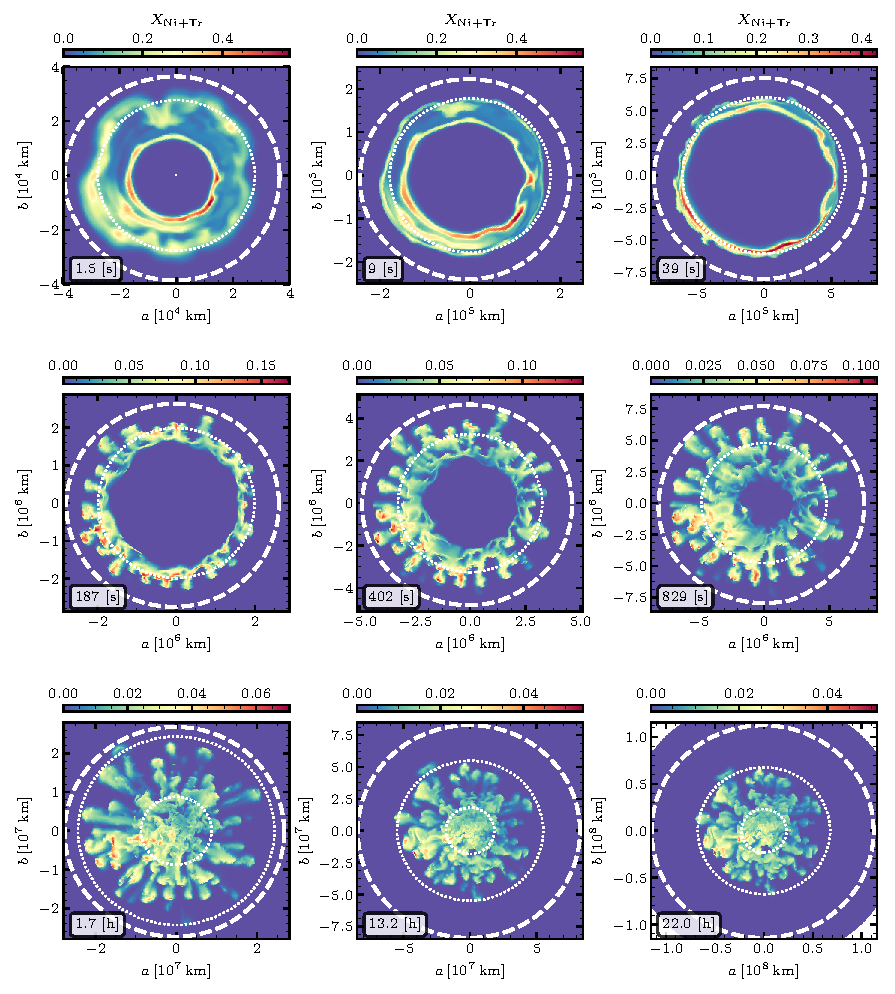
\includegraphics[width=\textwidth,trim=0cm 1.5cm 0cm 0cm,clip]{pic/z9_3d_3x3_NiX.pdf}
 \caption{Same as Figure~\ref{fig:e8 3d 4times} but for model $z9.6$. The dashed line indicates the shock radius. During the first $\tpb\mathord{\sim} 10\,\s$ the initial neutrino-heated high entropy plumes are compressed in a similar fashion as found in model $e8.8$. At $\tpb\mathord{\sim}40\,\s$ the initial structures have completely vanished and the first RT-plumes begin to grow from seed perturbations at the CO/He interface. While the finger grow, the reverse shock (visible at the bottom of the fingers) travels back into the innermost ejecta. Interestingly, the fastest RT plumes, which almost reach the supernova shock, seem the stem from the initially largest high entropy plumes (see panels at time $\tpb\mathord{=}1.5\,\s$ and $\tpb\mathord{=}829\,\s$).
 }
 \label{fig:z9 3d 4times}
\end{figure*}% Figure z9.6 slices

In Figure~\ref{fig:z9 3d 4times} we show planar cuts of the density distribution and $\nickel+\tracer$ mass fraction of the $z9.6$ similar to Figure~\ref{fig:e8 3d 4times}.
During the first $\sim 10\mathord{-}50\,\s$, the ejecta expand self-similarly into the He-shell of the progenitor, closely resembling the evolution of the ECSN simulation.
As can be seen in the upper right panel of Figure~\ref{fig:z9 3d 4times}, the self similar expansion is terminated at $t_{\mathrm{pb}}\approx 70\,\text{s}$.
When fastest metal rich ejecta arrive at the dense shell, they are compressed and induce high $\ell$-mode density perturbations at the CO/He interface, from which the first small RT-plumes grow.
Note that these initial fingers grow in a region confined between the forward shock and the dense shell that has formed due to the deceleration of the shock in the CO and He core. The bulk of the metal rich ejecta is located downstream of this dense wall.

While the fingers grow during the next $300-400\,\s$, the continuous deceleration of the shock in the He core sends pressure waves back into the post-shock material. Consequently, matter steepens into a reverse shock. The position of the reverse shock is visible as the color discontinuity in the lower left panel of Figure~\ref{fig:z9 3d 4times}. Since only small amounts of neutrino heated ejecta could be mixed outward before the reverse shock forms, the bulk of the iron group material is decelerated strongly.
At around $\tpb=1500\,\s$ the reverse shock reaches our inner boundary and is reflected back into the core material.
Consequently, non-linear waves perturb the innermost ejecta, distorting the Rayleigh-Taylor fingers that reached down to the inner boundary. 
After these dynamic events the forward shock reaches the He/H interface at around $\tpb=2000\,\text{s}$. Since the core/envelope transition is very smooth and the post shock density rather uniform, no additional growth of the RTi is to be expected. Accordingly the plumes that grew from the CO/He interface propagate unimpared with the background flow. 
Interestingly, very fast shrapnels, which stem from the initially largest plumes, escape the deceleration by the reverse shock (see lower right panel of Figure~\ref{fig:z9 3d 4times}).


\subsection{Extent of mixing}
%e8.8
In Figure~\ref{fig:e8 massDis 4times} we show the distribution of elements in mass and velocity space at four representative times during our long-term simulation of the $e8.8$. The upper two rows represent the evolution until $300\,\text{s}$ when the nickel rich ejecta encounter the dense shell.
The bulk of the \nickel/\iron surpasses the carbon and oxygen rich layers in velocity space at $t_{\mathrm{pb}}=300\,\text{s}$, when the inner ejecta are pushed against the dense shell and the first cusps mix \nickel outward in velocity space. The dense shell, however, hampers mixing in mass coordinate.
The encounter of the neutrino-heated ejecta with the reverse shock causes an enormous deceleration. This is shown in the lower two rows in Figure~\ref{fig:e8 massDis 4times}. Where most of the iron rich material has velocities of $v_{\mathrm{Ni,X}}\mathord{\approx} 30\times10^3 \,\mathrm{km/s}$ at $t_{\mathrm{pb}}\mathord{=}300\,\text{s}$ these layers are decelerated to $v_{\mathrm{Ni,X}}\mathord{\approx} 2.5\times 10^3\,\mathrm{km/s}$ within some $5 \,\mathrm{h}$. The lower velocity tail of the iron group elements even has negative velocities. 
Compression of the innermost ejecta by the reverse shock is also evident in the distribution over mass coordinate. Where a small fraction of the neutrino heated ejecta is mixed to $M(r)\mathord{=}1.4\,\mathrm{M_{\odot}}$ until $t_{\mathrm{pb}}=21.800\,\s$, the bulk resides still at  $M(r)=1.35\,\mathrm{M_{\odot}}$ clearly separated from the carbon and oxygen that extends to $M(r)=1.47\,\mathrm{M_{\odot}}$ and is evenly distributed over the whole post shock region.

% Figure e8.8 mass distribution
\begin{figure*}
 \centering
 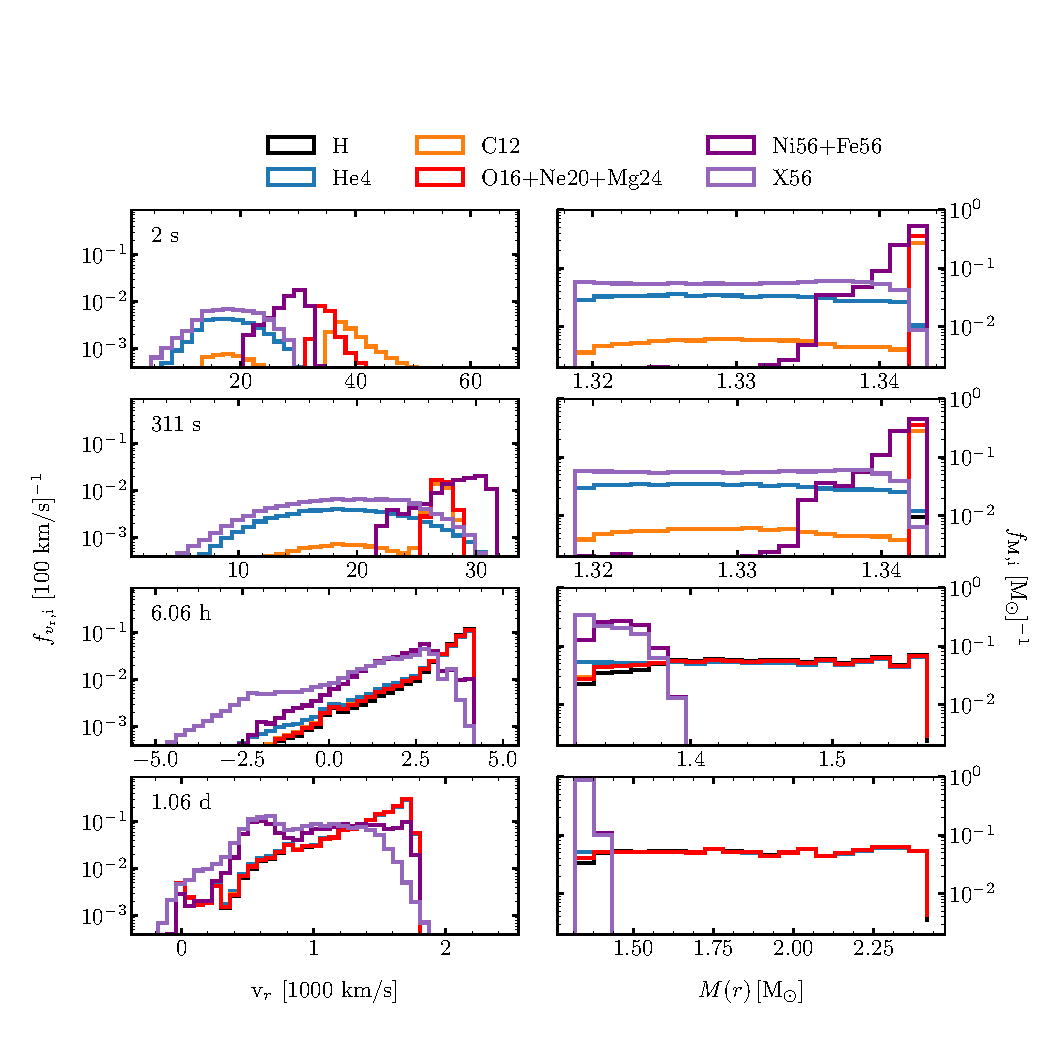
\includegraphics[width=\textwidth,trim=0cm 0.6cm 0cm 1cm, clip]{pic/e8_2d_10_massDis_mvr_mas_4times_paper.pdf}
 \caption{Mass distributions of elements in velocity and mass space  of the $e8.8^{\mathrm{2D}}_{10}$ model at the indicated post bounce times. We cover the initial state as we start our long term simulation in the uppermost panel, over the time the reverse shock passes the ejecta (second and third panels) and the distribution at late times.}
 \label{fig:e8 massDis 4times}
\end{figure*}
As has been stated before, the early formation of the dense shell has important consequences for the velocities the metal rich ejecta can achieve and how far they can be mixed into the envelope.
In Figure~\ref{fig:z9 massDis} we show the distribution of elements over mass and velocity space for the $z9.6$ model at the same snapshots as shown in Figure~\ref{fig:z9 3d  4times}, to illustrate the influence of the reverse shock and the dense shell onto the ejecta.

Compression of the ejecta in velocity space and some mixing over mass coordinate can be observed during $t_{\mathrm{pb}}\mathord{=}0.65\,\s$ and $t_{\mathrm{pb}}\mathord{=}78\,\s$. The compression is caused by the strong deceleration of the forward shock in the stellar material, reducing the initial maximal velocities from $v\mathord{\sim} 25\mathord{\times}10^3\,\mathrm{km/s}$ down to $v\mathord{\sim} 12.3\mathord{\times}10^3\,\mathrm{km/s}$, whereas the first plumes that rise from the CO/He interface mix a tiny amount of iron rich ejecta into the He-core. Note however that the reverse shock travels with $v_{\mathrm{rev}}\mathord{\sim} 7\mathord{\times}10^3\,\mathrm{km/s}$ at $t_{\mathrm{pb}}\mathord{=}400\s$ and the bulk of $\nickel$ and $\tracer$ travels with smaller velocities of $v\mathord{\sim} 4\mathord{\times}10^3\,\mathrm{km/s}$. The behaviour of the model is again similar but less extreme as found in the ECSN model.

As the RT-plumes grow over the course of the following minutes, they continuously mix $\nickel$ and $\tracer$ into the He-core. This is shown in the third row left column of Figure~\ref{fig:z9 3d 4times}. At the same time the reverse shock forces the bulk of the metal rich ejecta to even lower velocities of  $v\mathord{\sim} 0.5\mathord{\times}10^3\,\mathrm{km/s}$. The passage of the reverse shock also marked the point in time where the integrates growth rates of the $z9.6$ saturate. As can be seen in the lowest panels of Figure~\ref{fig:z9 3d 4times}, during the time between  $7.7\mathord{\times} 10^3\;\s$ and $6.4 \mathord{\times} 10^4\,\s$ neutrino-heated material experiences almost no additional upwards mixing in mass and is only further compressed in velocity space.
\begin{figure*}% Figure Z9.6 mass distribution
 \centering
 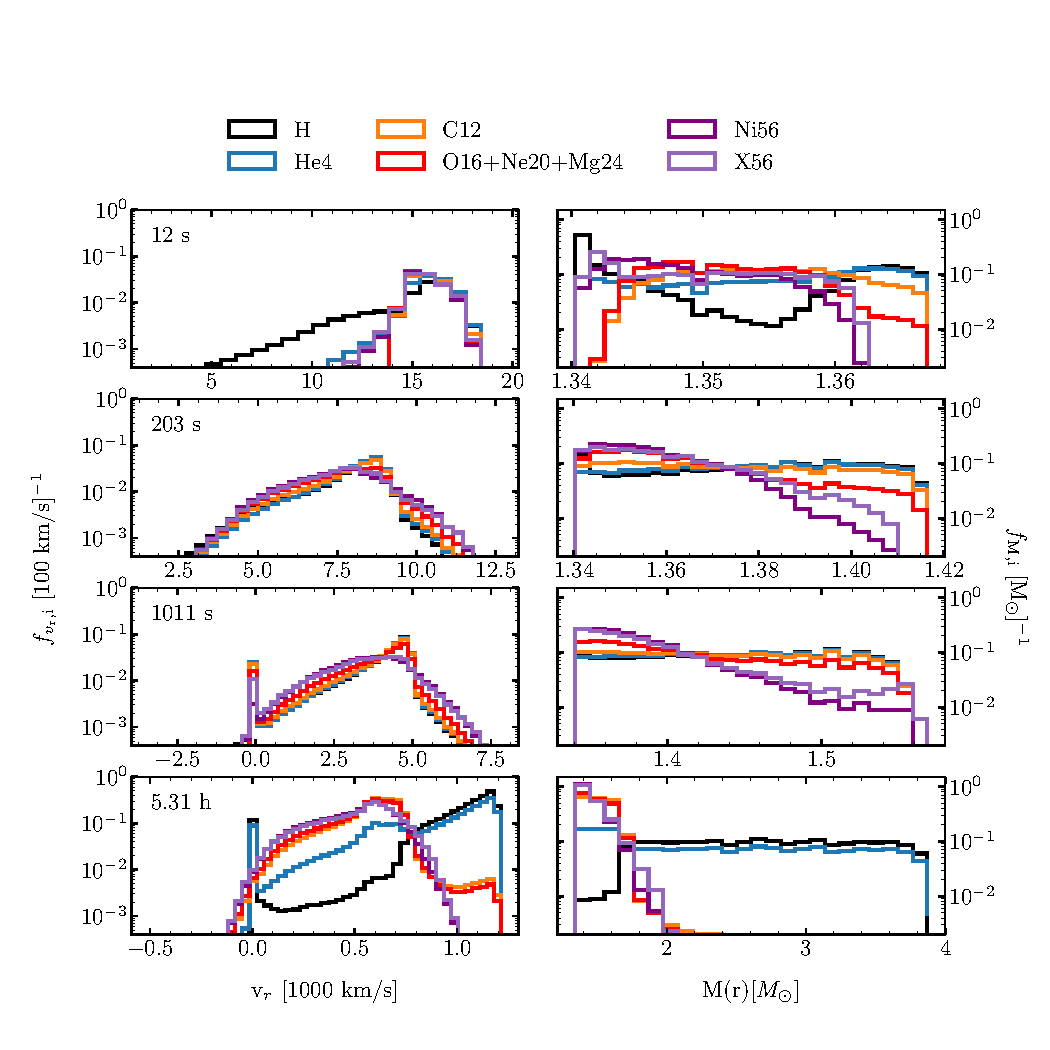
\includegraphics[width=\textwidth,trim=0cm 0.6cm 0cm 1cm,clip]{pic/z93_3d_massDis_mvr_mas_4times_paper.pdf}
 \caption{Same as Figure~\ref{fig:e8 massDis 4times} but for the $z9.6$ model. We cover the initial state as we start our long term simulation in the uppermost panel, over the time the reverse shock passes the ejecta (second and third panels) and the distribution in the hydrogen envelope as the ejecta expand self similarly.}
 \label{fig:z9 massDis}
\end{figure*}

\iffalse

\subsection{Multi-dimensional evolution of the }
\subsubsection{$z9.6$ Model}
\label{sec:Long term evolution of the z9.6 model}
% z9.6 1D
The 1D simulation of the $z9.6$ was initialized using spherically averaged values obtained from the 3D model\footnote{The recombination of leftover neutrons and protons from the \vertex simulation produced a very small transient, which has no impact on further evolution.} at $\tpb\,\mathord{=}\,1.40\,\s$. At this time \NY{the}{} the forward shock $(R_{\text{s}}\,\mathord{=}\,3.84\times 10^4\, \km)$ \NY{just passed the former}{ leaves the} C/He interface \NY{beginning its journey through}{ behind, and starts propagating across} the He-core.

During the next $10\, \s$, the dynamical evolution of the ejecta is dominated by the neutrino-driven wind, which accelerates material in the vicinity of the PNS to supersonic velocities. The fast \NY{}{moving} material eventually encounters the hot and dense matter behind the forward shock, and is strongly decelerated launching the so-called ``wind termination shock'' \citep{Wanajo2002,Arcones2007}. 

\NY{When}{ As} the energy input by the neutrino-driven wind subsides, the wind termination shock \NY{falls back}{ withdraws back} and leaves the \NY{}{inner} grid \NY{at our inner}{} boundary at $\tpb\,\mathord{\approx}\,12\,\s$.
Note that the strength of the neutrino driven wind, that is almost non-existent in the ECSN case, sets the maximum velocities the iron rich material can achieve and prevents strong deceleration of the forward shock in the envelope \citep{Wongwathanarat2015}. 

Similar to the evolution of the forward shock in the hydrogen layer of the ECSN progenitor, continuous deceleration of the forward shock in the He layer causes the formation of a reverse shock fairly early at some $\tpb\mathord{\approx} 100\,\s$. Until $\tpb\mathord{\approx}\, 300\,\s$ forward and reverse shock travel with roughly equal velocity through the He-core, where $\mathrm{R_{revsh}\mathord{\sim 0.72}\,\times R_{sh}}$. 
Again, the shocks clearly separate two different regimes in the ejecta. The inner neutrino heated ejecta bounded by the thin dense shell at the reverse shock and the lower density material between the shocks which is prone to the RTi (see Section~\ref{sec:Linear Stability Analysis}).
%
After $300\,\s$ after bounce, the between forward and reverse shock decreases until the reverse shock reaches the inner boundary at $t_{\mathrm{pb}}\sim 1.14\,\text{h}$. This is more than 4 hours earlier than in the $e8.8$ case. The passing of the reverse shock compresses the inner ejecta and leaves behind a low density bubble rather than a constant density profile as found in the electron-capture case.
The interaction of the reflected reverse shock with the ejecta is also more dynamic as in the $e8.8$ model. Non-linear waves travel back and forth bounded by the inner computational boundary and high density neutrino-heated ejecta. From here, matter expands until the time of shock-breakout at $\tpb\approx\, 29\,\mathrm{h})$. %


\subsubsection{$s9.0$ Model}
\label{sec:Long term evolution of the s9.0 model}
\COM{Not Final}
Given that the $s9.0$ model is fairly asymmetric compared to the zero metallicity progenitor or the electron capture model, the angle averaged model for the 1D simulation shows a smoothed out density and velocity profile and thus a smoothed out shock. Thus results from this simulation are even more qualitative than for the other two cases.
When the forward shock leaves the CO-core it accelerates to its maximum value of $0.8\times 10^{9}\mathrm{cm/s}$ . As it travels through the He4 shell it is decelerated piling up matter in a dense shell behind it. When it reaches the H/He4 interface ($\sim 200$ [s]) the drop in density sends a pressure wave back into the ejecta that steepens into a reverse shock. Note that this reverse shock begins to fall back relatively late at around 22 [h] and reaches the inner boundary as late as 37 [h]. The reflected shock wave runs back into the ejecta while at 90 [h] the forward shock breaches the surface of the star. Due to this the density structure looks quite different to the $z9.6$ model. The large cavity is less pronounced and confined by a dense shell at its lower boundary. 


\subsection{ONeMg-core progenitor}
%\subsubsection{$e8.8$ Model}
\label{sec:Long-term evolution of the e8.8}

In the lower right panel of Figure~\ref{fig:density all times} we show the forward and reverse shock trajectory of the $e8.8$.


\subsection{Multi-dimensional long-term evolution of the $e8.8$}
\label{sec:Multi-dimensional long-term evolution of the e8.8}
\subsubsection{Shock propagation}
\label{sec:shock propagation e8.8}
We show in Figure~\ref{fig:density all times} the angle-averaged density distributions at representative epochs alongside with the forward and reverse shock trajectories of our three-dimensional simulations. Red markings in the density distribution indicate Rayleigh-Taylor unstable regions. In the lower two panels we show the ECSN case.

The forward shock has long passed the He/H interface and is traveling through the H-envelope. It left the ONeMg-core with some $7.5\times 10^{9}\,\text{cm/s}$ and now travels at $5.8\times 10^{9}\mathrm{cm/s}$. The monotonic $\rho r^3$-profile of the $e8.8$ leads to an untroubled expansion of the shock.

The early and strong deceleration of the forward shock at the edge of the ONeMg-core at $\tpb=0.17\,\text{s}$ has formed a high density shell, bounded by a reverse shock at its inner shoulder. It separates the post shock material from the innermost ejecta as can be seen in the lower left panel of Figure~\ref{fig:density all times}, where we show the density stratification of our three-dimensional models at representative epochs. The formation of the dense shell or ``wall'' \cite{Kifonidis2006} has important consequences for the evolution of the metal rich ejecta as well as for the growth of Rayleigh-Taylor instabilities. 

Continuous deceleration of the forward shock eventually causes the reverse shock to travel back in mass, starting at  $\tpb\mathord{\approx}\,1\text{h}$ (see lower right panel of \ref{fig:density all times}). It takes however additional $7\,\text{h}$ for the reverse shock to reach the inner boundary of our computational domain. 
Unaffected by the processes in the interior, the forward shock travels through the hydrogen envelope converting almost 50\% of its kinetic energy into heating the hydrogen gas. Due to this and the huge size of the envelope ($R_{\mathrm{surf}}\mathord{\approx}8.8\times10^{13}\,\mathrm{cm}$) shock-breakout occurs between 3 and 5 days depending on the energy input by the central engine. At this time the shock travels with about $v_{\mathrm{sh}}\mathord{\approx} 5\times 10^{7}\, \mathrm{cm/s}$ accelerating to some $2.6\times 10^{8}\, \mathrm{cm/s}$ as it leaves the star.

The high density shell, that formed during the enormous deceleration at the core/envelope interface, is visible in the lower left panel of Figure~\ref{fig:density all times} at $\tpb=2.5\,\s$ just behind the forward shock at $R_{\mathrm{sh}}=1.77\times10^{5}\,\km$. 
Note that the region around this shell is unstable to the RTi but contains only very little mass.
Continuous deceleration of the forward shock in the hydrogen envelope compresses and decelerates the post-shock material (see Figure~\ref{fig:density all times} from $\tpb\mathord{=}2.5\,\s$ until $\tpb\mathord{=}3092\,\s$). Consequently the reverse shock is pushed back in radius and mass coordinate as can be seen in the lower right panel of Figure~\ref{fig:density all times}. 
Further evolution of the forward and reverse shock is identical to the spherically symmetric results presented in Section~\ref{sec:Long-term evolution of the e8.8}. 

\subsubsection{Ejecta morphology}
% self similar expansion
As mentioned in Section~\ref{sec:Post-Bounce Evolution of the e8.8 Model}, the neutrino-heated ejecta basically freeze in their angular distribution starting from $\tpb\mathord{=}0.4\,\s$ and expand self-similar into the low density H-envelope (see lower panels of Figure~\ref{fig:e8 sto 4 times}). 

A shell of \nickel, created by explosive burning behind the shock front \citep{Kifonidis2006}, propagates in front of the homogenous neutron/tracer rich inner core material. The boundary between \nickel/\tracer still carries imprints of the high entropy buoyant bubbles, which grew during strong neutrino heating, whereas the outer boundary of the \nickel shell traces the spherical shock expansion. In the two-dimensional simulations the plumes have angular sizes of some $30^{\circ}$, whereas they are more prolate and smaller in their angular extend in the three-dimensional simulation. 
While the almost spherical shock will induce only tiny density perturbations on the post-shock layers, these plumes carry slightly larger density perturbations from which the RTi grows. Note, however, that these perturbations are still very small and the density profile shows only tiny differences to the one-dimensional simulation.

In Figure~\ref{fig:e8 3d 4times} we show planar cuts of the density of the ECSN model at representative epochs. Indicated by the black contour line is the \nickel+\tracer=0.1 iso-surface. It traces the region of neutrino-heated material. The dashed white line indicates the $M(r)=M_{\mathrm{He/H}}$ mass shell.

The first Rayleigh-Taylor plumes grow from the tiny perturbation that arose from the passage of the forward shock. These are barely visible in the density distribution, however. 
When the self-similarly expanding plumes eventually catch up with the immediate post-shock matter at around $\tpb\mathord{=}30\,\s$, they induce high $\ell$-mode perturbations at the RT-unstable core/envelope interface (see orange discontinuity in the uper right panel of Figure~\ref{fig:e8 3d 4times} close to the core/envelope interface). 
Subsequent growth of Rayleigh-Taylor plumes fully mix the thin \nickel rich shell into the surrounding layers. It looses any resemblance with its morphology at $\tpb\mathord{=}0.3\,\s$. 
Over the following $\tpb\mathord{\sim}6.1\,\text{h}$ Rayleigh-Taylor plumes grow around the core/envelope interface. This is shown in the lower left panel of Figure~\ref{fig:e8 3d 4times}.
Rayleigh-Taylor plumes are clearly visible at the \nickel+\tracer iso-surface.
Note, that the tips of plumes are still close to the former core/envelope interface and amplification factors are almost saturated at this point in time (see Section~\ref{sec:Linear Stability Analysis}). Thus, almost no growth of the RTi is observable between $\tpb\mathord{\sim} 6.1\,\text{h}$ and  $\tpb\mathord{\sim} 25.5\,\text{h}$.
The passage of the reverse shock, visible as the blue discontinuity in the lower left panel of Figure~\ref{fig:e8 3d 4times}, compresses the inner region and drags the lower boundary of the RT-plumes to smaller radii. Parasitic instabilities and non-linear waves that originate from the reflection of the reverse shock at the inner boundary fully obliterate the metal rich ejecta leaving no trace of the initial plume structure (see lower right panel of Figure~\ref{fig:e8 3d 4times}). 

\subsubsection{Extend of mixing}
\begin{figure*}% Figure e8.8 rho cuts
 \centering
 \includegraphics[width=\textwidth,trim=0.2cm 2cm 0cm 0cm,clip]{pic/e8_both_slices_4times.pdf} 
 \caption{Planar cuts through the $e8.8_{\mathrm{2D}}$ model at the indicated times showing the logarithm of the density (left half) and \nickel+\tracer mass fraction (right half). Note that the shock radius is outside the shown domain. Expansion happens self similarly over until first RT fingers grow at the He/H interface. These fingers grow to their maximal radial extent when the reverse shock, located at the lower end of the RT fingers in the lower left panel, travels back to the center of the star.}
 \label{fig:e8 3d 4times}
\end{figure*}
When the metal rich ejecta catch up with the forward shock, they also are decelerated by a huge amount.
In Figure~\ref{fig:e8 massDis 4times} we show the distribution of elements in mass and velocity space at four representative times during our long-term simulation. The upper two rows represent the evolution until $300\,\text{s}$ when the nickel rich ejecta encounter the dense shell.
The bulk of the \nickel/\iron surpasses the carbon and oxygen rich layers in velocity space at $t_{\mathrm{pb}}=300\,\text{s}$, when the inner ejecta are pushed against the dense shell and the first cusps mix \nickel outward in velocity space. The dense shell, however, hampers mixing in mass coordinate.
The encounter of the neutrino-heated ejecta with the reverse shock causes an enormous deceleration. This is shown in the lower two rows in Figure~\ref{fig:e8 massDis 4times}. Where most of the iron rich material has velocities of $v_{\mathrm{Ni,X}}\approx 30\times10^3 \,\mathrm{km/s}$ at $t_{\mathrm{pb}}=300\,\text{s}$ these layers are decelerated to $v_{\mathrm{Ni,X}}\approx 2.5\times 10^3\,\mathrm{km/s}$ within some $5 \,\mathrm{h}$. The lower velocity tail of the iron group elements even has negative velocities. 
Compression of the innermost ejecta by the reverse shock is also evident in the distribution over mass coordinate. Where a small fraction of the neutrino heated ejecta is mixed to $M(r)=1.4\,\mathrm{M_{\odot}}$ until $t_{\mathrm{pb}}=21.800\,\s$, the bulk resides still at  $M(r)=1.35\,\mathrm{M_{\odot}}$ clearly separated from the carbon and oxygen that extends to $M(r)=1.47\,\mathrm{M_{\odot}}$ and is evenly distributed over the whole post shock region.

% Figure e8.8 mass distribution
\begin{figure*}
 \centering
 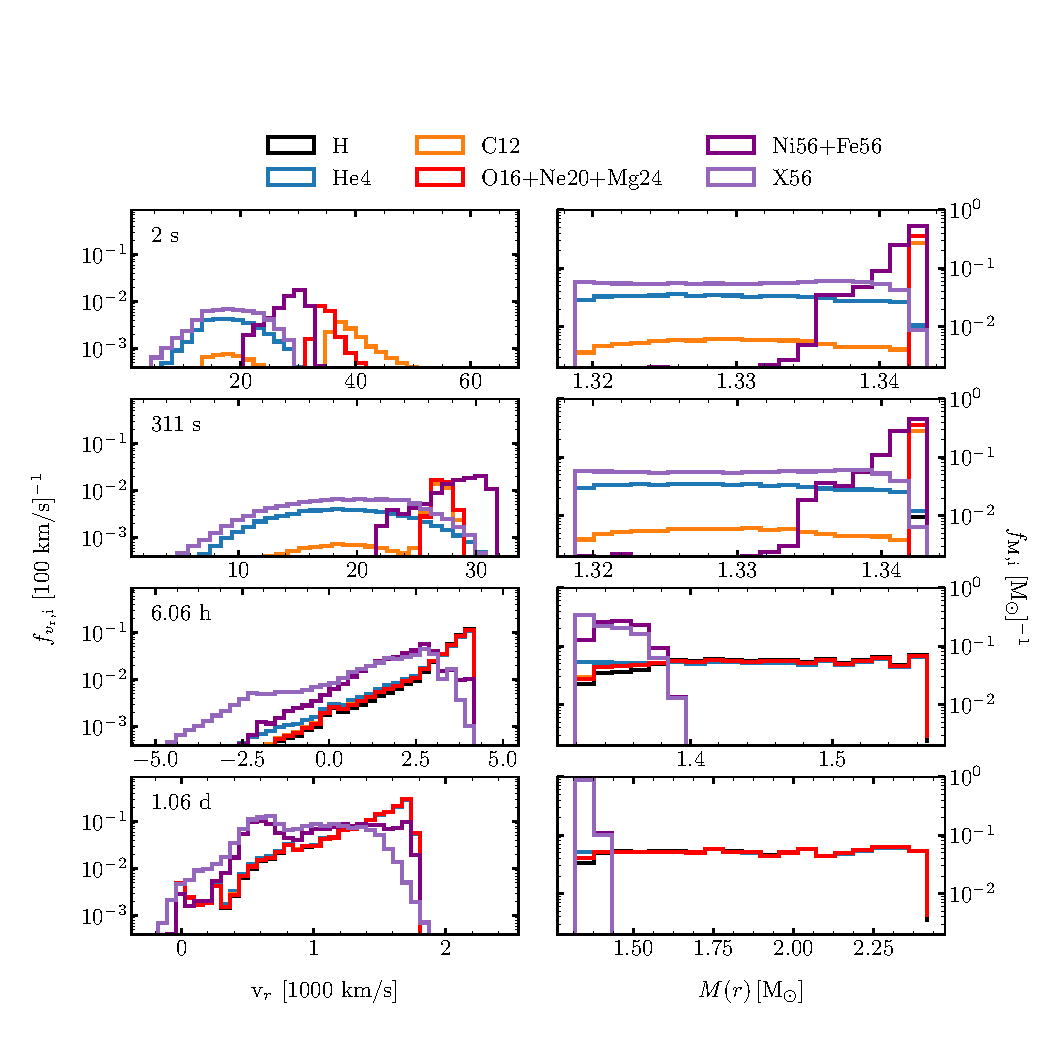
\includegraphics[width=\textwidth,trim=0cm 0.6cm 0cm 1cm, clip]{pic/e8_2d_10_massDis_mvr_mas_4times_paper.pdf}
 \caption{Mass distributions of elements in velocity and mass space  of the $e8.8^{\mathrm{2D}}_{10}$ model at the indicated post bounce times. We cover the initial state as we start our long term simulation in the uppermost panel, over the time the reverse shock passes the ejecta (second and third panels) and the distribution at late times.}
 \label{fig:e8 massDis 4times}
\end{figure*}

\iffalse %UNCOMMENTED
%post shock breakout
After shock breakout the very first stage of the remnant evolution begins. As long as the ejecta mass is larger as the circumstellar - mass (CSM) swept up by the forward shock one speaks of the ejecta dominated (ED) phase. Various analytical studies regarding shock evolution and growth of instabilities have been focusing around this phase (see e.g. \cite{Truelove1999} for a general approach or focused around the crab \cite{Chevalier1984}).  It is also the phase where, after radioactive decay has powered the plateau phase of type II supernovae, the medium becomes optically thin and the remnant moves into the nebular phase. Here velocity distributions also of the heavy elements can be inferred by spectral analysis of the ejecta.
\fi %UNCOMMENTED

\subsection{Multi-dimensional long-term evolution of the $z9.6$}
\label{sec:Multidimensional long term evolution of the z9.6}
\subsubsection{Shock propagation}
The propagation of the forward and reverse shock of the $z9.6$ model is shown in the upper right panel of Figure~\ref{fig:density all times}. The upper left panel shows the angle-averaged density distribution of the same model.
Deceleration of the forward shock in the He-core of the $z9.6$ compresses the post-shock matter and creates a high density shell. The shell can be seen in the density distribution at $\tpb\mathord{\sim}40\,\s$. Similar to the ECSN model, the region in the vicinity of this shell is unstable to the RTi but only consists of little mass.
As the forward shock continues to expand, a reverse shock forms at the lower edge of the dense shell between $\tpb\mathord{\sim}40\mathord{-}300\,\s$. 
Before the He/H interface is reached by the forward shock, the reverse shock already travels back in mass coordinate and compresses the core material. 
% Figure Z9.6 rho cuts
\begin{figure*}
 \centering
 \includegraphics[width=\textwidth,trim=0cm 1.5cm 0cm 0cm,clip]{pic/z9_contour_both_4times.pdf}
 \caption{Same as Figure~\ref{fig:e8 3d 4times} but for the $z9.6_{\mathrm{3D}}$. The dashed line indicates the shock radius. Initially the \nickel+\tracer distribution is fairly spherical with small deformations in the south-western direction. These deformations are reduced as the material expands. First RT-cusps are visible at $t_{\mathrm{pb}}\approx 200\,\text{s}$, whilw the reverse shock, visible as the reddish discontinuity at $r\approx 2\times 10^{6}\,\mathrm{km}$ already travels back in radius.}
 \label{fig:z9 3d 4times}
\end{figure*}

\subsubsection{Ejecta morphology}
In Figure~\ref{fig:z9 3d 4times} we show planar cuts of the density distribution of our three-dimensional simulation of the $z9.6$ similar to Figure~\ref{fig:e8 3d 4times}. Indicated by the dashed white line is the CO/He interface of the progenitor. The black line again shows the \nickel+\tracer=0.1 iso-surface, that carries the imprints of convective motions during the explosion.

During the first $\sim 10\mathord{50}\,\s$, the ejecta expand self-similarly into the He-shell of the progenitor, closely resembling the evolution of the ECSN simulation.
As can be seen in the upper right panel of ~\ref{fig:z9 3d 4times}, the self similar expansion is terminated at $t_{\mathrm{pb}}\approx 70\,\text{s}$.
When fastest metal rich ejecta arrive at the dense shell, they are compressed and induce high $\ell$-mode density perturbations at the CO/He interface, from which the first small RT-plumes grow.
Note that these initial fingers grow in a region confined between the forward shock and the dense shell that has formed due to the deceleration of the shock in the CO- and He-core. The bulk of the metal rich ejecta is located downstream of this dense wall.

While the fingers grow during the next $300-400\,\s$, the continuous deceleration of the shock in the He-core sends pressure waves back into the post-shock material. Consequently, matter steepens into a reverse shock. The position of the reverse shock is visible as the color discontinuity in the lower left panel of Figure~\ref{fig:z9 3d 4times}. Since only small amounts of neutrino heated ejecta could be mixed outward before the reverse shock forms, the bulk of the iron group material is decelerated strongly.
At around $\tpb=1500\,\s$ the reverse shock reaches our inner boundary and is reflected back into the core material.
Consequently, non-linear waves perturb the innermost ejecta, distorting the Rayleigh-Taylor fingers that reached down to the inner boundary. Since the reflected wave cannot catch up with the fastest shrapnels that originated from the growth of RT plumes at the CO/He interface, it does not influence the high velocity iron rich ejecta.
After these dynamic events the forward shock reaches the He/H interface at around $\tpb=2000\,\text{s}$. Since the core/envelope transition is very smooth and the post shock density rather uniform, no additional growth of the RTi is to be expected. Accordingly the plumes that grew from the CO/He interface propagate unimpared with the background flow. 
% Figure Z9.6 mass distribution
\begin{figure*}
 \centering
 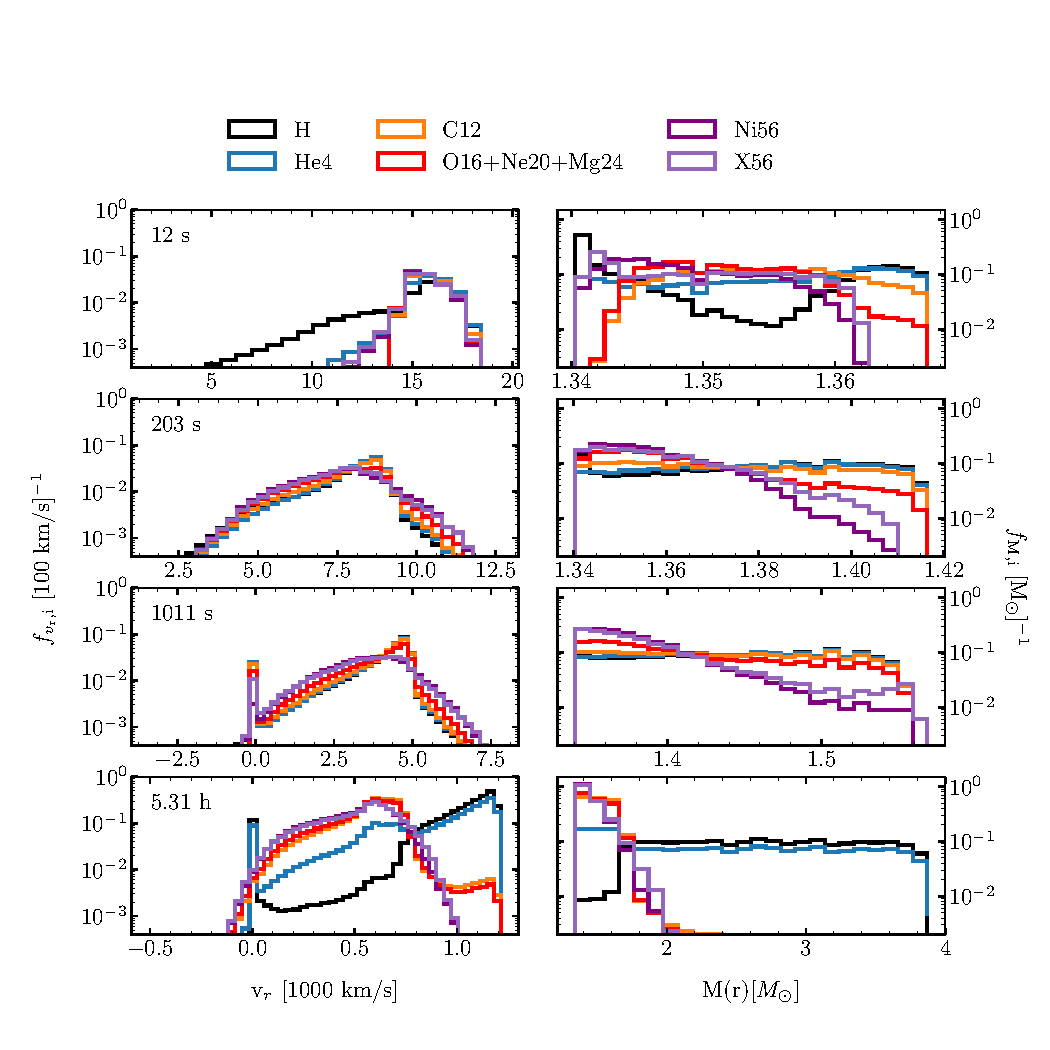
\includegraphics[width=\textwidth,trim=0cm 0.6cm 0cm 1cm,clip]{pic/z93_3d_massDis_mvr_mas_4times_paper.pdf}
 \caption{Same as Figure~\ref{fig:e8 massDis 4times} but for the $z9.6_{\mathrm{3D}}$. We cover the initial state as we start our long term simulation in the uppermost panel, over the time the reverse shock passes the ejecta (second and third panels) and the distribution in the hydrogen envelope as the ejecta expand self similarly.}
 \label{fig:z9 massDis}
\end{figure*}

%\subsubsection{Extend of Mixing}
\subsubsection{Extent of mixing}
As has been stated before, the early formation of the dense shell has important consequences for the velocities the metal rich ejecta can achieve and how far they can be mixed into the envelope.
In Figure~\ref{fig:z9 massDis} we show the distribution of elements over mass and velocity space for the $z9.6$ model at the same snapshots as shown in Figure~\ref{fig:z9 3d  4times}, to illustrate the influence of the reverse shock and the dense shell onto the ejecta.

Compression of the ejecta in velocity space and some mixing over mass coordinate can be observed during $t_{\mathrm{pb}}=0.65\,\text{s}$ and $t_{\mathrm{pb}}=78\,\s$. The compression is caused by the strong deceleration of the forward shock in the stellar material, reducing the initial maximal velocities from $v\approx 25\times10^3\,\mathrm{km/s}$ down to $v\approx 12.3\times10^3\,\mathrm{km/s}$, whereas the first plumes that rise from the CO/He interface mix a tiny amount of iron rich ejecta into the He-core. Note however that the reverse shock travels with $v_{\mathrm{rev}}\approx 7\times10^3\,\mathrm{km/s}$ at $t_{\mathrm{pb}}=400\s$ and the bulk of \nickel and \tracer travels with smaller velocities of $v\approx 4\times10^3\,\mathrm{km/s}$. The behaviour of the model is again similar but less extreme as found in the ECSN model.

As the RT-plumes grow over the course of the following minutes, they continuously mix \nickel and \tracer into the He-core. This is shown in the third row left column of Figure~\ref{fig:z9 3d 4times}. At the same time the reverse shock forces the bulk of the metal rich ejecta to even lower velocities of  $v\approx 0.5\times10^3\,\mathrm{km/s}$. The passage of the reverse shock also marked the point in time where the integrates growth rates of the $z9.6$ saturate. As can be seen in the lowest panels of Figure~\ref{fig:z9 3d 4times}, during the time between  $7.7\times 10^3\;\s$ and $6.4 \times 10^4\,\s$ neutrino-heated material experiences almost no additional upwards mixing in mass and is only further compressed in velocity space. 

\subsection{Multi-dimensional long-term evolution of the $s9.0$}
\label{sec:Multi-dimensional long-term simulations of the s9.0-model}
\COM{
\begin{itemize}
    \item Growth of RTi at He/H
    \item Initial perturbations growing from passage of O interfaces
\end{itemize}
}
\fi % MULTI - D EVOLUTION

\subsection{Dependence on the explosion energy}
\label{sec:Dependence on the explosion energy}
% e8.8
\iffalse
\begin{figure*}
 \centering
 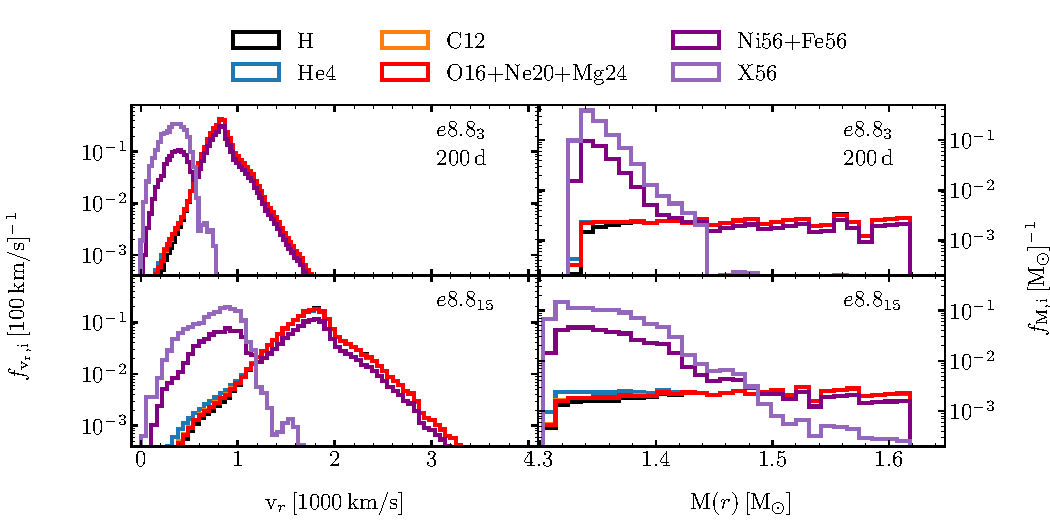
\includegraphics[width=0.95\textwidth]{pic/massDis_mvr_mas_minmax_2d_time_200d_paper.pdf}
 \caption{Mass and velocity distributions of elements at 200 days after bounce for the two dimensional models $e8.8_{3}$ and $e8.8_{15}$. We used 100 bins evenly distributed from $0-4\times 10^3\,\mathrm{km/s}$ and 30 bins in mass coordinate. The $e8.8_{3}$ calibration is the model with least efficient mixing, whereas the $e8.8_{15}$ is the model with most efficient mixing within our set of simulations of the $e8.8$. Thus, there is a small but noticeable dependence of the efficiency of mixing on the explosion energy. }
 \label{fig:e8 massDis 200 d}
\end{figure*}
\fi
Although the explosion energies for the e8.8 model cover almost one order of magnitude, differences in mixing of species in radius and velocity are minor. At $t_{\mathrm{pb}}\sim 2.5 \,\text{s}$ the velocity distribution of elements is almost identical. Small differences are visible in the maximum velocities achieved and are higher for higher explosion energy. Mixing in mass coordinate follows a similar pattern, with slightly more \nickel mixed into the neutron rich material for more energetic explosions. 
Inspecting later times ($t_{\mathrm{pb}}\sim 8 \,\mathrm{h}$) the findings still show similar behaviour. \nickel is mixed over a slightly larger fraction of the total ejected mass for the higher explosion energies. Differences in the velocity distribution are only visible in the lower tail with negative velocities. 
At 200 days after core bounce the velocity distributions are, besides the maximum velocities, basically identical.
% iron-cores
As the ion core progenitors are exploded self consistently their explosion energy is fixed within our framework. Drawing direct connections between the amount of mixing and the explosion energy can therefore not be done. Comparing the $z9.6$ model with electron-capture model, that have similar explosion energies, hints that the influence is, however, minor. Decisive for the amount of nickel mixing is the progenitor structure and initial perturbations after shock revival. This view is supported by the strong mixing apparent in the $s9.0$ model that has comparable explosion energy as well. The initial density perturbations combined with the strong de- and acceleration of the forward shock in the envelope of the progenitor yields high growth-rates over a larger space in mass coordinate. 
\COM{Effect of expl. energy, if iron rich material can be accelerated more efficient to escape the formation of the reverse shock. -> Interdependence of the strength of the wind and prog. structure. }

\subsection{Dependence on progenitor structure and initial morphology}
\COM{
\begin{itemize}
    \item Correlation fastes Ni plumes at \tpb=0 and \tpb= breakout?
    \item progenitor: early deceleration in ECSN like prog. s9.0 reverse shock only at He/H interface. 
\end{itemize}
}
In the previous sections we revealed the vast differences of the propagation of the forward shock and of the neutrino heated material between the three progenitors. 
Dependent on the core structure, the morphology of the ejecta at the moment of shock revival gradually changes from  almost spherical, as in the $e8.8$ model, to large scale anisotropies, as the $s9.0$ model.
The subsequent evolution depends strongly on the time the reverse shock forms and on the density gradient at the composition interfaces.
Early formation of the reverse shock at the core/envelope boundary in the $e8.8$ model suppresses efficient outward mixing of metal rich ejecta. When the reverse shock falls back, the inner material is compressed loosing every resemblance with its morphology at $\tpb=2.5\,\s$.
In the $z9.6$ model the situation is similar, although not as severe. A more gradual change in the $\rho r^3$ profile enables some outward mixing of \nickel, while the forward shock runs through the He core. Still, the back propagation of the reverse shock affects most of the neutrino heated material. Only a few shrapnels of \nickel and \tracer manage to escape the large deceleration. These shrapnels seem to originate from the largest plumes observed at the time of shock revival. This is no surprise as they most efficiently seed density perturbations necessary for the RTi to grow \citep{Wongwathanarat2015}.

\COM{$S9.0$ Details}

Summarizing it can be stated, that the progenitor features which enable fast explosions in our ECSNe like models, also prevents efficient mixing of core material. The forward shock is decelerated early on, causing a formation of a dense shell and a reverse shock that. In the $e8.8$ model no individual \nickel/\tracer shrapnels can escape deceleration of the reverse shock. In the $z9.6$ model very few shrapnels survive. 
\section{Comparison to previous studies}
\label{sec:Comparison to previous studies}

Previous studies like the ones of \cite{Hammer2010}, \cite{Joggerst2010}, \citet{Wongwathanarat2015}, \citet{Kifonidis2006} also performed simulations of the long term evolution of CCSNe after shock revival. These studies employed RSG and BSG progenitors as a proxy for Sanduleak -69 202, the progenitor of SN1987A. \citet{Hammer2010} used a 15 \solm blue supergiant, while \citet{Joggerst2010} used three different 15 \solm progenitors with different metallicities. Also the study by
\citet{Wongwathanarat2015} (Wo15) deployed various models from 15 - 20 \solm. 
Since these progenitors are more massive than the ones presented in this study, their structure is fairly different. E.g. the lightest CO-core of Wo15, their model B15, has a mass of $1.7\solm$ whereas our heaviest CO-core, our $s9.0$ model has a mass of $1.4\solm$. Additionally density gradients at the interfaces seem to be more pronounced especially at the He/H transition. Only our $s9.0$ model shows a noteworthy density variation at this interface.

However the total growth rates of the RTi seem to be unaffected as shown in Figure ~\ref{fig:growth rates}. The $s9.0$ model exhibits similar amplification factors as the models presented Wo15. Especially regions affected by the passage of the reverse shock show considerable growth factors. This is not mentioned in Wo15 and contributes to the total amount of mixing in the $s9.0$ model. Consequently neutrino heated material can be mixed far into the hydrogen envelope. 
Since the amplification factors of the ECSN like models are large but confined into a small region close to their core, these models are distinct from all other RSGs. Similar to the models presented in \citet{Joggerst2010} metal rich ejecta can be mixed only to a mass coordinate of around 15-20\% of the progenitors ZAMS mass.
\COM{
\begin{itemize}
    \item Conclude: Our models show that there is a transition from ECSNe like and low metallicities to low mass iron-cores (solar metallicity) to higher mass models
    \item Extrapolations and correlations ?
\end{itemize}
}

\section{Conclusions and Outlook}
In the present paper we presented the results of two- and three-dimensional simulations of CCSNe connecting the seconds after bounce, shock revival and shock breakout. We used three low-mass progenitors, two RSGs that produced an iron-core at the end of their life ($z9.6$, $s9.0$) and a newly explored ECSN progenitor ($e8.8$). 

The explosion of the $e8.8$ in one-, two- and three dimensions was initiated by imposing suitable values for neutrino luminosities and mean energies at the inner grid boundary located at a finite, time-dependent radius. Neutrino transport and neutrino-matter interactions were treated by the RbR gray neutrino transport scheme of \citet{Scheck2006}, including a improvement of the prescription for neutrino source terms as presented in the appendix. We confirmed the common behavior of ECSNe already presented in e.g. \citet{Kitaura2006,Gessner2018}. Early decline of the mass accretion rate leads to early explosions and fast shock expansion at the edge of the ONeMg-core even in one-dimension. Shock trajectories are fairly independent of the chosen geometry, while the almost spherical expansion produces only small PNS kicks of the order of a few \kms. Additionally convective motions in the multi-dimensional simulations are too weak and short-lasting to enable efficient mixing of neutrino-heated matter early on.

The immediate post bounce evolution of the iron-core models was simulated with \vertex employing a fully self consistent neutrino transport scheme. A detailed analysis of the first second of evolution of the $z9.6$ is given in \citet{Melson2015a}, while the $s9.0$ as firstly presented in \citet{Melson2019}. 
In addition to these studies we showed the hydrodynamic PNS kicks of these CCSN and investigated the morphology of the ejecta some hundred milliseconds after shock revival. 

When mass accretion subsides in all models and explosion energies and kick velocities begin to saturate we map the final state of our explosion simulations into \prom. This is achieved by excising the inner almost spherically symmetric regions of the previous simulations and replacing them by a suitable point mass. By incorporating the neutrino-driven wind and setting the radius of the inner boundary below the sonic point we guarantee a seamless transition between the codes.

At the time when we continue the simulations of the explosions the forward shocks of all three dimensional models traveled already more than $10^9\,\mathrm{cm}$. 
In order to aid us understand the growth of Rayleigh-Taylor instabilities in the multi-dimensional models we ran spherically symmetric simulations with the same setup starting from angle-averaged initial states. As expected amplification factors are large at the composition interfaces where the shock speed is non-monotonic. Not reported by previous three-dimensional studies is the additional amplification in region between the interfaces that is revealed using the compressible estimation of $\Sigma_{\mathrm{RT}}$.

As mentioned by \citet{Wongwathanarat2015} the evolution of the forward shock and neutrino-heated ejecta is very complex. De- and acceleration of the shock at the composition interfaces causes pressure inversions in the post-shock material that provide the ground for the growth of Rayleigh-Taylor instabilities, while the pile-up of matter behind the shock leads to the formation of dense shells and a reverse shock. 
In the case of the ECSN like progenitors the dense shells form early during the evolution. In the extreme case of the $e8.8$ the extreme deceleration of the shock at the ONeMg-core boundary compresses the post shock material already at 170 ms. The resulting dense wall is almost impermeable for the neutrino heated ejecta. When they catch up with the dense shell they are strongly decelerated and only imprint small scale low amplitude perturbations there. 
In the $z9.6$ model the forward shock has not passed the He/H interface before a strong reverse shock forms. Although some metal rich ejecta can penetrate through the previously formed dense shell most of the neutrino heated material remains within the radius of reverse shock formation.
The $s9.0$ model shows a different behaviour caused by the different structure structure of the star. Similar to the RSGs presented in Wo15 reverse shock formation happens after passage of the He/H interface while the Rayleigh-Taylor instabilities have enough time to grow to considerable size. Thus more neutrino heated material can be transported from the core to larger mass coordinates. 
In this study we identify three different morphologies.
The ECSNe like progenitors show only small derivations from sphericity duing their whole evolution after bounce.

The $e8.8$ model in particular does not produce large scale RTi fingers that are able to mix neutrino-heated material into the envelope. This is due to the very small initial perturbations set by convective overturn during the first roughly 200 ms after bounce and the monotonic shock propagation in its hydrogen envelope. 

The $z9.6$ model yields a very similar distribution of elements in mass and angular domain. Different to the ECSN progenitor however some metal rich shrapnels are able to escape the formation of the reverse shock and propagate unimpared behind the forward shock front. These shrapnels are correlated with the biggest initial plumes that originated from the evolution during the first second. The model thus represents a transition between two extremes. The completely spherical ECNS model and the $s9.0$ model.

The $s9.0$ model occupies a different regime in our results. A long accretion phase in combination with strong convective motions during the first second set large scale initial perturbations for the RTi to grow. The very late formation and fallback of the reverse shock guarantees the survival of large Rayleigh-Taylor fingers that mix neutrino-heated material outwards. 


\begin{itemize}
    \item \COM{These differences should be detectable in light-curve measurements of IIP transients. [Sashas Paper]}
    \item \COM{Correlation between rt fingers and initial plumes?}
    \item \COM{Distinction in nickel velocities?}
    \item \COM{Effect of $\beta$ decay}
    \item \COM{Effect of pre-collapse perturbations}
\end{itemize}

\section*{Acknowledgements}
\begin{itemize}
    \item Computational resources
    \item Financial Support
    \item Tools: NumPy, Matplotlib
    \item Naveen for input
\end{itemize}

%-----------
% BIB
% --------------
\bibliographystyle{mnras}
\bibliography{bibtex}       % name your BibTeX data base

\newpage
%----------
% APPENDIX
% --------------
\appendix
\section{PNS cooling model and inner boundary condition in \prom}
\label{Appendix:prom inner boundary}
As stated in Section~\ref{sec:Collapse and post-bounce setup in prom} we use the modeling approach presented in \cite{Ugliano2012} and \cite{Sukhbold2016}. 
The central 1.1 \solm of the PNS is excised from the computational domain and replaced by a contracting inner grid boundary $R_{\mathrm{ib}}$. The shrinking of the cooling and deleptonizing PNS is mimicked by the contraction of the inner grid boundary which is described by 
\begin{equation}
    R_{\text{ib}}(t) = R_{\text{ib,f}} + (R_{\text{ib,i}} - R_{\text{ib,f}})\, \exp\left(-\frac{t}{t_0}\right),
\end{equation}
where $R_{\text{ib,f}}$ is the final radius, $R_{\text{ib,i}}$ the initial radius and $t_0$ the timescale. $R_{\text{ib,f}}$ and $t_0$ are two of our set of free parameters and are chosen to mimic the behavior of PNS contraction found in more advanced simulations of PNS cooling.
As detailed in \cite{Ugliano2012}, the PNS core of mass $M_{\mathrm{c}}\mathord{=}1.1\,\solm$ is described by an analytic one-zone model under the constraints of energy conservation and the virial theorem including the effects associated with the growing pressure of the accretion layer, whose accumulation around the PNS core is followed by the hydrodynamic simulations. The one-zone model provides the time-dependent neutrino luminosities at $R_{\mathrm{ib}}$ which are given by 
\begin{equation}
\begin{split}
\label{eqn:lib}
    L_{\mathrm{\nu,tot}} = & - \frac{2}{5} \frac{3\Gamma - 4}{3(\Gamma - 1)} \frac{GM^2_{\mathrm{c}} R_{\mathrm{c}}}{R_{\mathrm{c}}^2} \\
            &  - \frac{3\Gamma - 4} {3(\Gamma - 1)} \frac{aGM_{\mathrm{c}}\Delta m_{\mathrm{acc}}R_\mathrm{c}}{R^2_{\mathrm{c}}}  -\frac{aGM_{\mathrm{c}}\Delta m_{\mathrm{acc}}R_{\mathrm{c}}}{3(\Gamma - 1)R_{\mathrm{c}}}.
\end{split}
\end{equation}
Here $\Gamma = 3$ is the adiabatic index of the PNS core (assumed to be homogeneous), $G$ is the gravitational Newton's Gravitational constant, $M_{\mathrm{c}}$ is the core mass, $a$ is a parameter which characterizes the accretion luminosity, and $\Delta m_{\mathrm{acc}}$ is the mass contained between the PNS radius $R_\mathrm{c}$ and the radius at which the density falls below $10^{10}\gcc$. In multi-dimensional simulations, $\Delta m_{\mathrm{acc}}$ is determined from angle-averaged values.
The time dependence of the core radius follows a power-law 
\begin{equation}
    R_{\mathrm{c}}(t) =R_{\text{c,f}} + (R_{\mathrm{c,i}} - R_{\mathrm{c,f}}) \left(1+\frac{t}{t_{\text{L}}}  \right)^p,
\end{equation}
where $t_L \mathord{=} 1 \, \text{s}$ and $p \mathord{<}0$ and  initially $R_{\mathrm{c,i}}\mathord{=}R_{\mathrm{ib}}$. Note that the PNS radius may not coincide with the radius of the inner boundary at all times.
In sum $p$, $R_{\mathrm{ib,f}}$, $a$, $R_{\mathrm{c,f}}$ and $t_0$ constitute our set of parameters to approximate the physics of the time evolution of the PNS and to enable explosions also in spherical symmetry.
The calibration of these parameters was done using the method described in \citet{Ertl2016}.

\section{Additions to the Neutrino transport module in \prom}
\label{Appendix:Neutrino}
\iffalse
\NY{Since there have been some modifications in the transport module of Prometheus-HotB}{ In this section, we will describe the modifications in the transport module of \prom}. \NY{we summarize}{ We will first summarize} the \NY{basis}{ basic} treatment \NY{here again}{ for the sake of completeness}. \NY{A more thorough description is to be found in }{ The interested reader should refer to} \cite{Scheck2006} (S06 hereafter) \NY{}{for details}. \NY{As described in S06 the}{ The} transport of neutrinos in Prometheus-HotB is approximated by an analytical solution of the zeroth angular moment of the spherically symmetric \NY{Boltzmann-Transport Equation}{ Boltzmann's transport equation}. The energy and angle integrated equation for the luminosity $L=4\pi r^2 F$ reads
\begin{equation}
\label{equ:transport1}
\frac{\partial L}{\partial t} + c_{\mathrm{eff}} \frac{\partial L }{\partial r} = 4 \pi r^2 c_{\mathrm{eff}} (Q^+ - Q^-)
\end{equation}
Here $c_{\mathrm{eff}}$ is the effective speed of the propagating neutrinos and $Q^+$, $Q^-$ are the source and sink terms.
Integrating \ref{equ:transport1} yields the analytic solution for the transport equation
%%
\begin{equation}
%\label{equ:transport2}
\begin{split}
L(r,t) = \, & L(r^*,t^{*}) e^{- \tilde{\kappa} c_{\mathrm{eff}} (t-t^{*}) } + \frac{4\pi Q^{+}}{\tilde{\kappa}^3}\\
& \Big\{ [ 1 - e^{-\tilde{\kappa} c_{\mathrm{eff}} (t-t^{*} )} ] [ 1 + (\tilde{\kappa}r^{*} -1)^2 ] + \\
& \tilde{\kappa} c_{\mathrm{eff}} (t - t^{*} ) [ 2 \tilde{\kappa} r^{*} + \tilde{\kappa} c_{\mathrm{eff}} (t-t^{*}) - 2 ] \Big\}\\
\end{split}
\end{equation}
where the notation is the same as in S06.
To calculate the source terms an assumption about the neutrino energy spectrum and thus about the mean neutrino energy $\epsilon$ has to be made. S06 writes the energy dependency of the specific intensity as
\begin{equation}
\label{equ:intensity}
I_{\mathrm{\nu\{n,e\}}}(t,r,\epsilon,\mu) = \Big(\frac{\epsilon^{\{2,3\}}}{(hc)^3} \Big) c f_{\mathrm{D,\nu}}(t, r, \epsilon, \mu),
\end{equation}
where the exponents $2,3$ apply for number-, energy transport and $f_{\mathrm{D,\nu}}(t, r, \epsilon, \mu)$ is assumed to be a product of a Fermi-Dirac distribution $f_{\mathrm{D,\nu}}$
\begin{equation}
\label{equ:fermi-dirac}
f_{\mathrm{D,\nu}} = \frac{1}{1+exp(x-\eta)}
\end{equation}
and an angle-dependent function $g_{\nu}$
\begin{equation}
\label{equ:fermi-dirac-g}
f_{\mathrm{D,\nu}}(t, r, \epsilon, \mu) = g_{\nu}(r,t,\mu)f_{FD}\Big( \frac{\epsilon}{k_B T_{\nu}(r,t)},\eta_{\nu} \Big).
\end{equation}
Here $\eta_{\nu}$ is the neutrino-degeneracy parameter and $T_{\nu}$ is the neutrino temperature. Details on how these values are initialized and treated are described in more detail in S06. In order to compute the mean neutrino energies one needs the Fermi-Dirac integral

\begin{equation}
\label{equ:fermi-dirac-integral}
\mathcal{F}_{\mathrm{n}}(\eta) = \int_0^{\infty}dx x^n f_{\mathrm{FD}}(x,\eta),
\end{equation}

giving also the neutrino energy moments

\begin{equation}
\label{equ:energy-moments}
\langle \epsilon^{\mathrm{n}}_{\nu} \rangle = (k_{\mathrm{B}} T_{\nu})^{\mathrm{n}} \frac{\mathcal{F}_{\mathrm{2+n}}(\eta_{\nu})}{\mathcal{F}_{\mathrm{n}}(\eta_{\nu})}.
\end{equation}

The energy averaged neutrino source- and sink terms are calculated as given in S06 at every timestep and are incorporated in the factors $Q^+$ and $\tilde{\kappa} $ respectively.
\fi

\subsection{Correction to Neutrino-Nucleon Scattering}
Due to numerical issues in the neutrino transport module of \prom, long-term simulations ($\tpb\mathord{>3\,\s}$) including the neutrino transport, showed spurious oscillations in the source terms $Q_{\nu}$. Especially cases where no are very late explosion was observed were affected. 
This was caused by an inconsistency  in the treatment of the Neutrino-Nucleon Scattering.
\cite{Scheck2006} use the scattering term calculated by \cite{Tubbs1979}
\begin{equation}\label{equ:nns}
\begin{aligned}
Q_{\mathrm{\nu N}} = \, & \frac{1}{4} \mathcal{C}_N \mathcal{E}_{\mathrm{N}} \frac{n_{\mathrm{N}}}{m_{\mathrm{N}}c^2}
\{\langle \epsilon^4 \rangle - 6 T\langle \epsilon^3 \rangle  \} \\
& \times  \frac{L_{e,\nu}}{4\pi r^2 f_{\nu}\langle \epsilon \rangle}\\
\end{aligned}
\end{equation}
which is their equation (D.68). Here $\langle \epsilon \rangle$ is again the mean neutrino-energy and $T$ the temperature of the thermal target in MeV.
In certain cases, the temperature exceeds $\langle \epsilon^4 \rangle / 6 \langle \epsilon^3 \rangle $ adding energy to the neutrinos. As the scattering term was implemented solely as an energy sink for neutrinos, the transport scheme became unstable, causing strong oscillations in the neutrino-fluxes. Due to the tight coupling of fluxes and source-terms, strong gradients in the fluxes cause a strong response in $Q^+$, $Q^-$. This unphysically heats up the material, creating additional luminosity and thus cooling of the PNS stops.
A simple solution to this problem is to separate the temperature-dependent term and split \ref{equ:nns} into two separate source-/sink terms
\begin{equation}\label{equ:nns1}
Q^{\mathrm{em}}_{\nu \mathrm{N}} = - \frac{6}{4} \mathcal{C}_{\mathrm{N}} \mathcal{E}_{\mathrm{N}} \frac{n_{\mathrm{N}}}{m_{\mathrm{N}}c^2}
T \langle \epsilon^3 \rangle \frac{L_{e,\nu}}{4\pi r^2 f_{\nu}\langle \epsilon \rangle}
\end{equation}

\begin{equation}\label{equ:nns2}
Q^{\mathrm{abs}}_{\nu \mathrm{N}} = \frac{1}{4} \mathcal{C}_{\mathrm{N}} \mathcal{E}_{\mathrm{N}} \frac{n_{\mathrm{N}}}{m_{\mathrm{N}}c^2}
\langle \epsilon^4 \rangle \frac{L_{e,\nu}}{4\pi r^2 f_{\nu}\langle \epsilon \rangle}.
\end{equation}

%% TODO
%% TEST FIGURES
\begin{figure*}
\centering
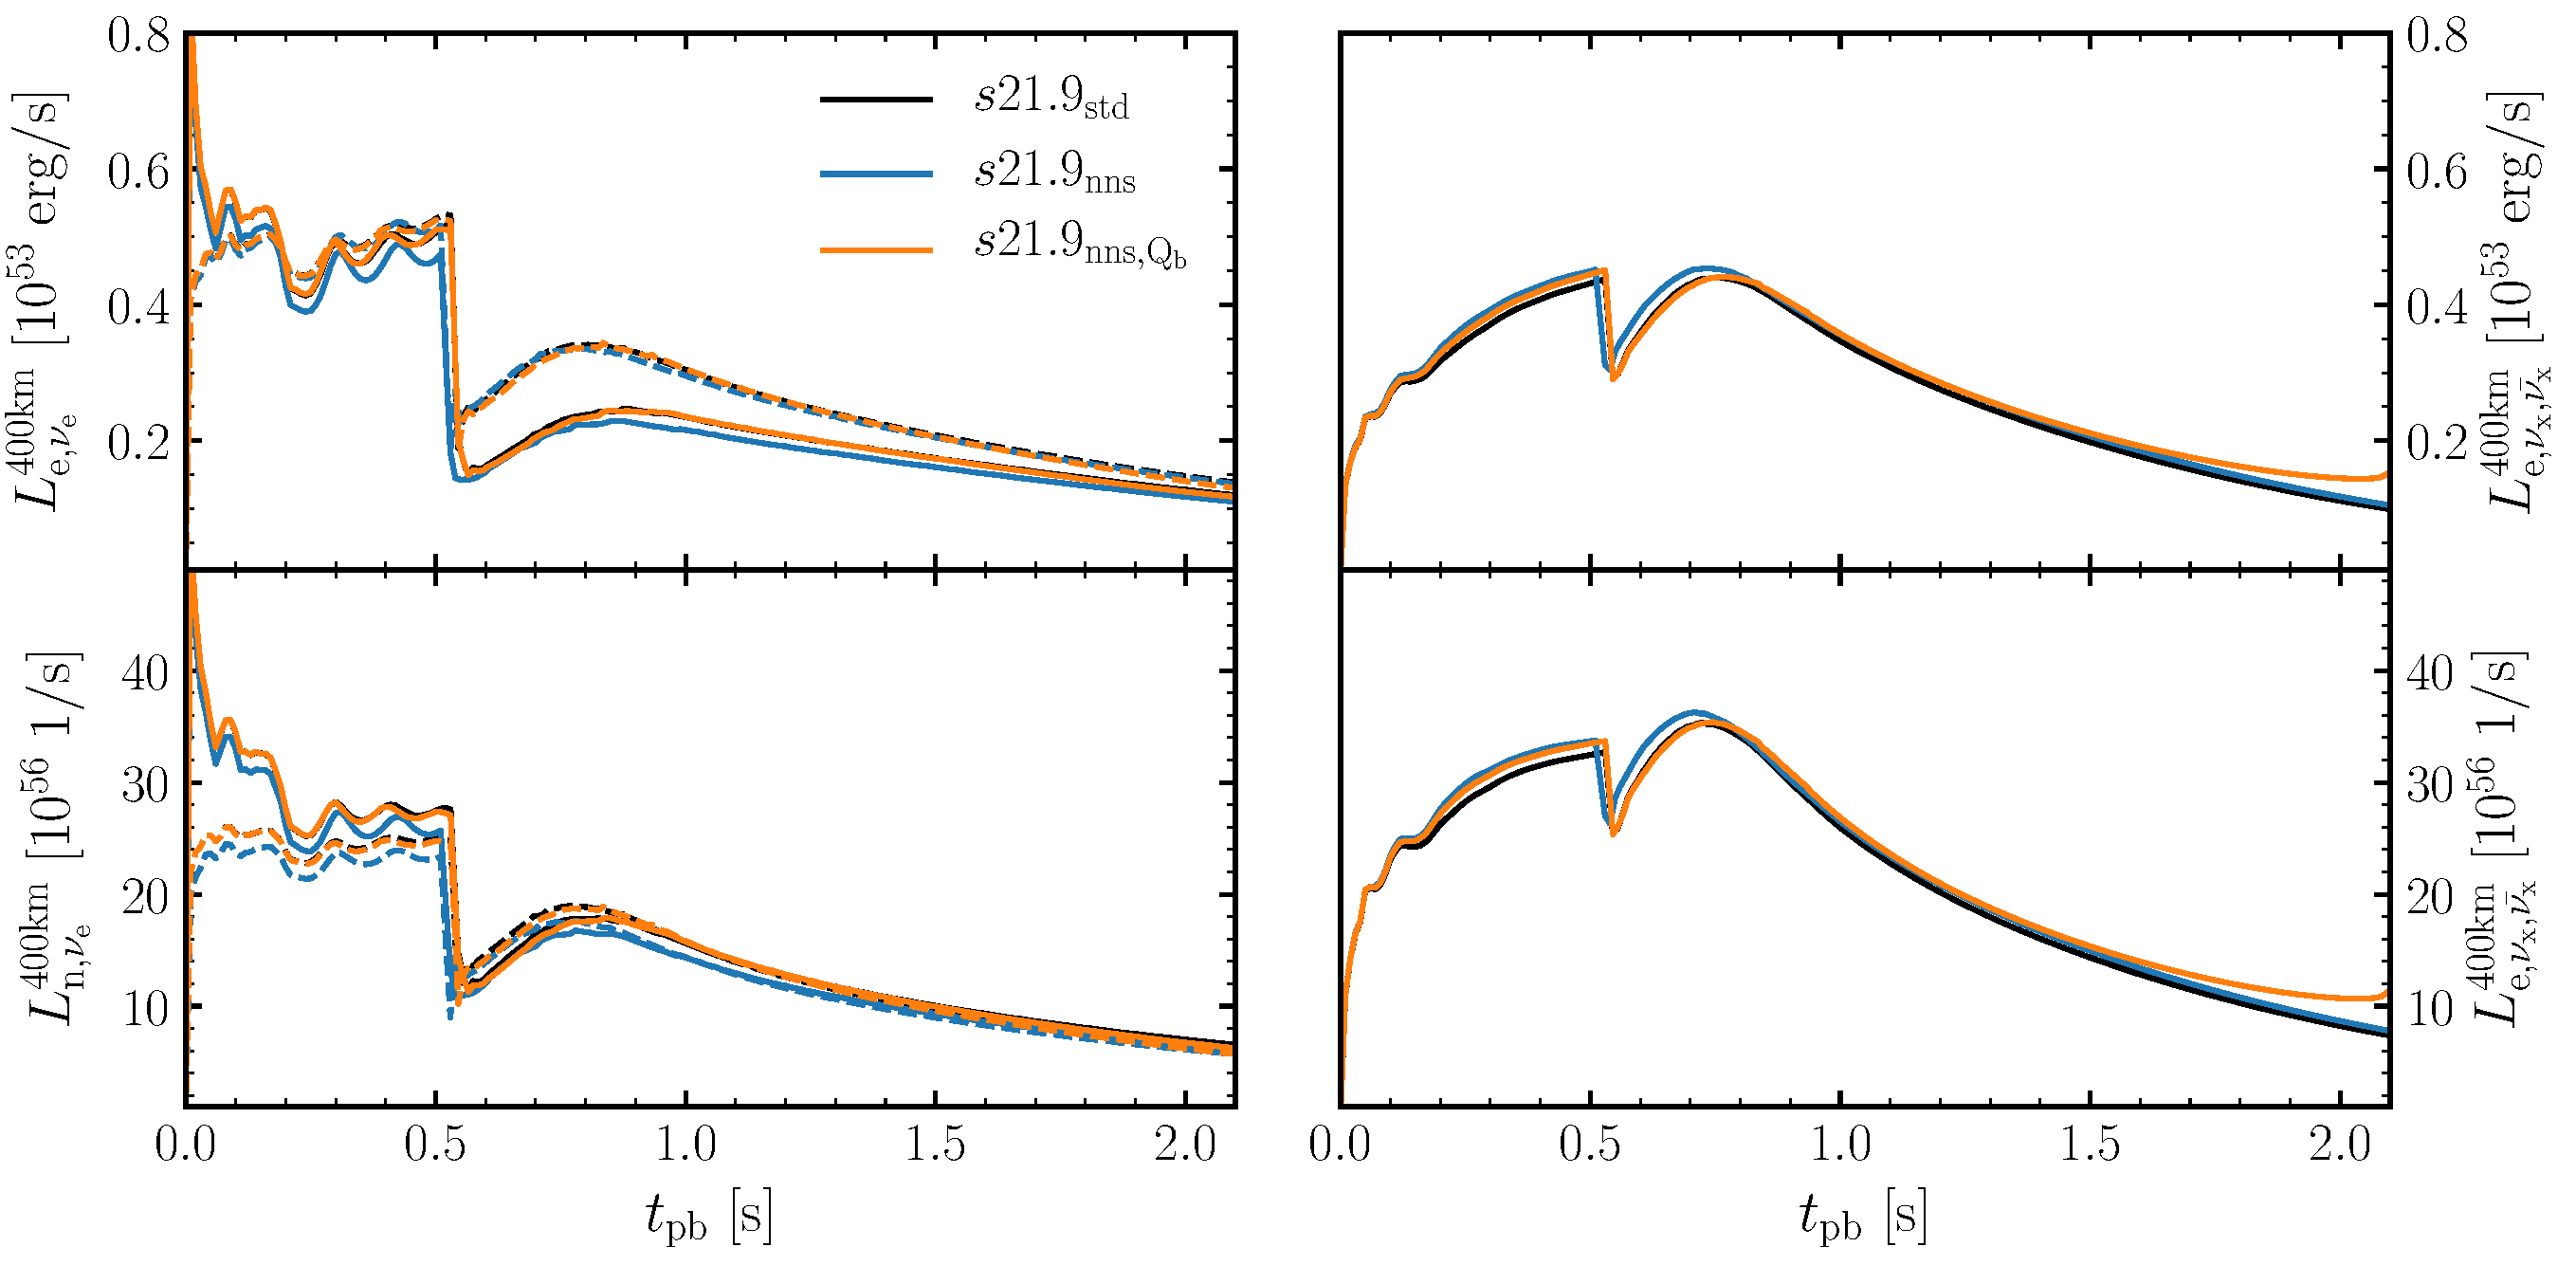
\includegraphics[width=0.8\textwidth]{./pic/s21_9_trans_tests.pdf}
\caption{Neutrino energy and number luminosities for a $21.9\,\mathrm{M_{\odot}}$ star using the transport of S06 ($s21.9_{\mathrm{std}}$), the corrected transport ($s21.9_{\mathrm{nns}}$) and including Bremsstrahlung ($s21.9_{\mathrm{std,Q_b}}$). \textit{Upper left panel}: Electron neutrino (solid lines) and electron anti-neutrino energy-luminosity at $400\,\mathrm{km}$. \textit{Lower left panel}: Electron neutrino (solid lines) and electron anti-neutrino number-luminosity at $400\,\mathrm{km}$. The left column of panels shows the same quantities for the heavy neutrinos ($\nu_{\mathrm{x}}$). Including the corrections presented here reduces the overall luminosities for this model. Adding Bremsstrahlung somewhat balances the reduction of $L_{\mathrm{e,n},\nu}$}
\label{fig:s21.9_tras}
\end{figure*}

\subsection{Bremsstrahlung}

In addition to the aforementioned improvements we now include neutrino Bremsstrahlung into our transport scheme. We follow the prescription given in \cite{Burrows2006}.
The total volumetric heating rate $ Q_{\mathrm{nb}}^{\mathrm{\nu_i}}$ by Nucleon-Nucleon Bremsstrahlung pair events, using the matter temperature $T$ and mass fractions $X_{\mathrm{n}}$, is given by

\begin{equation}
Q_{\mathrm{nb}}^{\mathrm{\nu_i}} = 0.5\cdot 1.04\cdot 10^{30} \xi \, \big(X_{\mathrm{n}}\rho_{14}\big)^2 (\frac{T}{\mathrm{MeV}})^{5.5} \,\, \Big[\frac{\mathrm{erg}}{\mathrm{cm^3s}}\Big],
\end{equation}
where $\rho_{14} = \frac{\rho}{10^{14}} \mathrm{\frac{g}{cm^3}} $
and $X_{\mathrm{n}}^2$ is defined as
\begin{equation*}
X_{\mathrm{n}}^2 = X_{\mathrm{neut}}^2 + X_{\mathrm{prot}}^2 + 28/3\, X_{\mathrm{neut}}X_{\mathrm{prot}}.
\end{equation*}

We add a factor of 0.5 in the above description as we calculate the energy generation by \textbf{one} neutrino and not by pairs of neutrinos. Here $\xi$ is a correction factor also set to 0.5.
For the energy loss $Q_{\mathrm{nb}}^{-}$ we assume
\begin{equation}
\frac{\kappa}{n_{\mathrm{b}}} = \frac{Q_{\mathrm{nb}}^{\mathrm{\nu_i}}}{c \epsilon^{\mathrm{eq}}} = \frac{Q_{\mathrm{nb}}^{-}\cdot 4\pi r^2 f_{\nu}}{L_{\nu}^{\mathrm{e}}}, 
\end{equation}
where $\kappa$ is the transport opacity as defined in S06, $n_{\text{b}}$ the baryon number density and $\epsilon^{\mathrm{eq}}$ is he mean neutrino energy assuming equilibrium conditions.
In the notation of S06 this yields
\begin{equation}
Q_{\mathrm{nb}}^{-} = \frac{Q_{\mathrm{nb}}^{\mathrm{\nu_i}} L_{\nu}^{\mathrm{e}} }{4\pi r^2 f_{\nu} c \epsilon^{\mathrm{eq}} n_{\mathrm{b}}}.
\end{equation}
For the Number emission we take
\begin{equation}
R=\frac{Q_{\mathrm{nb}}^{\nu_{\mathrm{i}}}}{\langle \epsilon \rangle} = Q_{\mathrm{nb}}^{\nu_i} \frac{L_{\nu}^n }{L_{\nu}^e }\,\, \mathrm{\frac{1}{cm^3s}}
\end{equation}
and for the absorption taking the equilibrium neutrino number density $n^{\mathrm{eq}}$ giving
\begin{equation}
n^{\mathrm{eq}} = \frac{8\pi T^3}{(hc)^3}\mathrm{F}_2.
\end{equation}
Here $\mathrm{F}_2$ is the Fermi-Dirac integral defined in Equation (D.23) in \cite{Scheck2006}.

%% TODO
%% SHOW TESTS
%% pair production should cool the material!

\section{Neutron star kicks and spin}
\label{Appendix:neutron star}
\subsection{Equations}
Acceleration of neutron stars are caused by two mechanisms. 
Asphericities developing during the explosion exert gravitational forces on the PNS which accelerate the PNS in the direction opposite of the direction of the explosion. This mechanism is also known as the ``gravitational tug-boat mechanism'' \citep{Wongwathanarat2013}. For a thorough discussion of this mechanism the reader is referred to \citet{Scheck2006,Wongwathanarat2013,Janka2017,Gessner2018,Mueller2019}.
Secondly, anisotropic emission of neutrinos, specifically the anisotropic neutrino energy flux density $F_{\mathrm{\nu}}^{\mathrm{e}}$ across the surface of the PNS, exerts a force onto the PNS in the direction opposite to the stronger neutrino emission.
Using the momentum conservation equation the hydrodynamic NS kick can be simply estimated as
\begin{equation}
  \pmb{\mathrm{P}}_{\mathrm{NS}} = \pmb{\mathrm{v}}_{\mathrm{NS}}\mathrm{M_{NS}} = -\pmb{\mathrm{P}}_{\mathrm{gas}},
\end{equation}
where $\mathrm{M_{NS}}$ is the baryonic (NS) mass contained inside the radius where the angle-averaged density drops below $10^{11}\, \gcc$ and $\pmb{\mathrm{P}}_{\mathrm{gas}}\mathord{=}\int_{_{R_{\mathrm{NS}}}}^{\infty} \rho\pmb{v}\ud V$ is the momentum of the ejecta outside the PNS.
The momentum transfer by neutrinos is given by
\begin{equation}
    \label{equ:nukick}
    \dot{\textit{\textbf{P}}}_{\nu} (t) = \oint_{r = R_\mathrm{gain}}
    \frac{F_{\nu}}{c}\ \textit{\textbf{e}}_r \, \ud S
    = - \dot{\textit{\textbf{P}}}_\mathrm{ns}^{\,\nu} (t) \,.
\end{equation}
Due to the RbR approximation in \vertexprom, only radial momentum flux has
to be considered.
Assuming the PNS mass does not change significantly ($\dot{M}_{\mathrm{NS}}\mathord{=}0$), and using $\textit{\textbf{P}}_\nu (t)\mathord{=}\int_0^{\, t} \dot{\textit{\textbf{P}}}_{\nu} 
(t')\mathrm{d}t'$, the velocity of the NS can be calculated as
\begin{equation}
  \pmb{\mathrm{v}}_{\mathrm{NS}}(t) = - \frac{\pmb{\mathrm{P}}_{\mathrm{gas}} + \pmb{\mathrm{P}}_{\mathrm{\nu}}}{ \mathrm{M_{NS}}}.
  \label{equ:momentum_kick}
\end{equation}.

One can connect the asymmetry of the ejecta and neutrino emission by the means of an anisotropy parameter. The hydrodynamic parameter reads 
\begin{equation}
    \alpha_{\mathrm{NS}} = \frac{|\mathbf{P}|_{\mathrm{gas}}}{P_{\mathrm{ej}}}
\end{equation}
where 
\begin{equation}
P_{\mathrm{ej}}=\int_{R_{\mathrm{NS}}}^{R_{\mathrm{sh}}}\rho |\mathbf{v}| \ud V
\end{equation}
is the total momentum stored in the ejecta.
For the neutrino anisotropy parameter we use 
the total energy loss rate in neutrinos, which is given by
\begin{equation}
\label{nuerg}
\dot{E}_\nu (t) = \oint_{r = R_\mathrm{gain}} F_{\!\nu}\, \ud S\,.
\end{equation}
The time dependent total flux of neutrino momentum through the sphere at 
$R_\mathrm{gain}$ is given by $c^{-1}E_\nu$ and allows one to define the
instantaneous neutrino emission anisotropy parameter as
\begin{equation}
\label{nuanis}
{\widetilde\alpha}_\nu (t) = 
c\,\frac{|\dot{\textit{\textbf{P}}}_{\nu}(t)|}{\dot{E}_\nu(t)}\,.
\end{equation}
In analogy to the ejecta momentum, the momentum radiated by neutrinos is
\begin{equation}
\label{pnu}
\frac{1}{c} E_\nu (t)
= \frac{1}{c}\int_0^{\, t} \oint_{r = R_\mathrm{gain}}F_{\!\nu}\, \ud S \mathrm{d}t'
\end{equation}
so that the integral neutrino emission asymmetry at time $t$ becomes
\begin{equation}
\label{anu}
\alpha_\nu (t) = c\,\frac{|{\textit{\textbf{P}}}_{\nu}(t)|}{E_\nu(t)}\,.
\end{equation}


In addition, we compute the NS spin by integrating the flux of angular momentum through a sphere of radius $r_0\,\mathord{=}\,500\,\km$ around the origin,
\begin{equation}
    \label{equ:jns}
    \frac{\mathrm{d}\mathbf{J}_{\mathrm{NS}}}{\mathrm{dt}} = r_0^2\int_{\Omega} \rho v_r \mathbf{v}\times \mathbf{r} \mathrm{d}\Omega,
\end{equation}
where $\rho$ is the density, $\mathbf{v}$ and $\mathbf{r}$ are the vector valued velocity and position and $v_r$ the radial velocity.

In order to estimate the spin period of the PNS $P_{\mathrm{NS}}=I_{\mathrm{NS}}/|J_{\mathrm{NS}}|$, with $I_{\mathrm{NS}}$ being the moment of inertia of the PNS, we use the approximation by \citet{Lattimer2004}
\begin{eqnarray}
    I_{\mathrm{NS}} &=& 0.237M_{\mathrm{g}}R_{\text{NS}}^2\left[1 + 4.2 A  + 90 A^4\right],\\
    A &=&  M_{\text{g},\solm}R_{\text{NS},\km}^{-1},\nonumber
    \label{equ: ins}
\end{eqnarray}
where $M_{\text{g},\solm}$ is the gravitational mass of NS in units of $\solm$, and $R_{\text{NS},\km}$ is the radius of the NS in units of $\km$.
In the above equation the gravitational mass $M_{\mathrm{g}}$ can be estimated from the baryonic mass $M_{\mathrm{b}}$  as \citep{Lattimer2000}
\begin{equation}
    M_{\mathrm{g}} = M_{\mathrm{b}} - \frac{0.6 \beta}{1-0.5\beta}  M_{\mathrm{g}}, 
\end{equation}
where $\beta=\frac{GM_{\mathrm{g}}}{R_{\mathrm{NS}}c^2}$ and
$M_{\text{b},\solm}$ is the baryonic mass of the NS.


\subsection{Results and discussion}
\begin{itemize}
    \item Plot $J_{ns}(t)$, $v_{hyd,\nu}(t)$, $\alpha_{hyd,\nu}(t)$...
\end{itemize}


\newpage

\label{lastpage}
\end{document}
% end of file template.tex

%% THRASH ->
\iffalse
% COMMENTED OUT
\subsection{Collapse}
\label{sec:Collapse}
The collapse of the iron-core progenitors was computed using the \vertex code and the collapse of the  electron-capture model was computed using the \prom code. While \vertex code uses its full neutrino transport during collapse,

\subsection{Post-Bounce Simulations}
\subsubsection{Iron-core progenitors}
The post-bounce modelling for the iron-core progenitors is done using \vertexprom, which is a finite-volume hydrodynamics code with three-flavor, energy-dependent, ray-by-ray-plus (RbR+) neutrino transport including the full set of neutrino reactions and microphysics as detailed in \cite{Rampp2002}. We use an axis-free YinYang-Grid \cite{Kageyama2004} implemented in \vertexprom by \cite{Melson2015a}. It  helps in relaxing the CFL time constraint caused by smaller cell size along the poles in a spherical polar grid. 

At densities above $10^{11}\,\gcc$ ($\rho_{\text{hd}}$) \vertex uses  the Equation of State (EOS) of \cite{Lattimer1991} with a nuclear incompressibility of $K=220\, \text{MeV}$. Below $\rho_{\text{hd}}$ \vertexprom uses the low-density EOS of \cite{Janka1999}. Above  temperatures greater than $5\times10^{9}$ ($T_{\text{NSE}}$ hereafter) nuclear statistical equilibrium (NSE) is assumed, whereas below $T_{\text{NSE}}$ a simple flashing scheme is used. The gravitational potential is computed in the monopole approximation, with appropriate general-relativistic corrections \citet{Marek2006}.

The region inside $10\,\text{km}$ is convectively stable, and is therefore simulated in 1D. \vertex preserves hydrostatic balance to machine precision, therefore in order to break the symmetry we impose random density perturbations with amplitude $10^{-3}$ at initial time. 
\subsubsection{ONeMg core progenitor}
The post-bounce evolution of the electron-capture progenitor is simulated using the \prom code (for details see \citealt{Wongwathanarat2012,Wongwathanarat2013}) For sake of completeness, we describe some features of the code and microphysics below.
\begin{itemize}
\item The code uses a grey (energy independent) neutrino-transport scheme, which is valid at low neutrino-opacities. In this scheme, the $\nu_{\mathrm{e,x}}$-fluxes are calculated by an analytic solution of the zeroth order moment of the Boltzmann equation as described in \citet{Scheck2006}\footnote{Improvements and corrections to the neutrino transport scheme \citep{Scheck2006} are given in the Appendix \ref{Appendix:Neutrino}.}. The most important details of this scheme are described in the next section.
% Gravity
\item The code uses a 3D gravitational potential with general relativistic corrections \citep{Marek2006}, which is achieved by using a multipole expansion of the integral form of Poisson's equation.
%nuclear reactions
\item A 17-species $\alpha$ reaction network keeps track of the nucleosynthesis up to $\mathrm{Ni}^{56}$. In order to capture the evolution of neutron rich matter ($Y_e\,\mathord{<}\,0.49$), we add a tracer species ($X$) to the network. Energy release by  nuclear burning is calculated, and added as a source term in the the energy conservation equation. 
Further, we use a flashing scheme to treat the recombination of free neutrons and protons leading to \helium production.
%Radioactive decay of Nickel
\item After shock-breakout the $\beta^{+}$-decay of radioactive \nickel becomes a dominant source of energy. 
%EOS
\item Similar to \vertex the high density EoS by \citet{Lattimer1991}  is used during the early stages of the explosion.For $\rho\,\mathord{<}\,\rho_{\mathrm{hd}}$, we use a slightly modified version of the Helmholtz-EoS \citep[includes Coloumb corrections due to electron-positron interactions]{Timmes1999}. Below the table boundaries of the standard Helmholtz-EoS ($\mathrm{\rho_{low}}\,\mathord{=}\,10^{-10}\, \gcc$, $T_{\mathrm{low}}\,\mathord{=}\,10^{4}\,\mathrm{K}$) we ignore the electron-positron interactions and the resulting EoS includes an effective Boltzmann gas and the radiation only. In the low density and low temperature regime, the pressure $p$, and the specific internal energy $e$ are given by
\begin{eqnarray}
    p &=& \frac{1}{3}aT^4 + \frac{\mathrm{k_b}}{\mu \mathrm{m_{H}}} \rho T, \\
    e &=& \frac{aT^4}{\rho} + \frac{3\mathrm{k_b}}{2\mu \mathrm{m_{H}}} T,\label{equ:pressure-energy-boltzmann-radiation}
\end{eqnarray}
where $a$, $\mathrm{k_b}$, $\rho$, $T$,$\mathrm{m_{H}}$, $\mu$ are the radiation constant, Boltzmann constant, density temperature, atomic mass unit and mean molecular weight respectively. Note that this approach assumes full ionization  and radiation pressure dominates in the shocked region \NY{}{CHECK THIS STATEMENT}.
\end{itemize}
%\subsubsection{Parametrization in Prometheus-HotB}
\subsubsection{Proto-Neutron Star (PNS) Contraction}\label{subsec:pnscontr}

After core bounce, the inner $0.5\, \solm$ of the core is excised, and replaced by a fixed boundary with hydrostatic boundary condition as in \citet{Ertl2016}. We impose constant neutrino luminosity until the forward shock reaches $1.25\, \solm$ in mass coordinates. This phase lasts for a few milliseconds after bounce. Thereafter, the PNS, which is the region inside $1.1\, \solm$ is  excised and replaced by a moving inner boundary. We impose hydrostatic boundary condition with respect to the moving inner boundary, and use a time dependent Lagrangian formulation on the computational grid outside $1.1\, \solm$. The kinematic evolution of the inner boundary radius is given by
\begin{equation}
    R_{\text{ib}}(t) = R_{\text{ib,f}} + (R_{\text{ib,i}} - R_{\text{ib,f}})\, \exp\left(-\frac{t}{t_0}\right),
\end{equation}
where $R_{\text{ib,i}}$ and $R_{\text{ib,f}}$ are the initial and the final radius of the excised $1.1\, \solm$ core, and $t_0$ \NY{the}{ is a} \NY{}{characteristic} timescale\NY{}{.} \NY{for the boundary movement.}{The value of $R_{\text{ib,i}}$ is obtained from simulation, whereas $R_{\text{ib,f}}$ and $t_0$ are treated as parameters.}
\NY{}{The PNS cools by emitting neutrinos and thereby contracts with time.} \NY{To model the time dependent cooling of the neutron star and thus the time dependent neutrino luminosities,}{} \NY{we}{ We} use the analytic model of \cite{Ugliano2012} \NY{}{to model the cooling and subsequent contraction of the PNS. In this model the PNS neutrino luminosity is obtained by an application of the First law of thermodynamics.} \NY{}{The total energy $E_{\text{c}}$ of the PNS (sum of the gravitational energy $E_{\text{g}}$ and the internal energy $E_{\text{i}}$) changes as a result of neutrino cooling and pressure-volume work done on the its surface, which can be expressed as 
\begin{equation}
    \dot{E}_{\text{c}} = - L_{\mathrm{\nu,c}} - 4\pi P_{\text{s}}R_{\text{c}}^2\dot{R}_{\text{c}},
\end{equation}
where $L_{\mathrm{\nu}}$ is the neutrino luminosity, $P_{\text{s}}$ is the pressure on PNS surface, $R_{\text{c}}$ is the PNS radius, and  $\dot{R}_{\text{c}}$ is the PNS contraction rate. Using the Virial theorem the total energy of the PNS core can be expressed as
\begin{equation}
    E_{\text{c}}= -\frac{3\Gamma -4}{3(\Gamma -1)}E_{\text{g}} + 
    \frac{4\pi R_{\text{c}}^3 P_{\text{s}}}{3(\Gamma -1)},
\end{equation}
Here $\Gamma = 3$ is the adiabatic index of the PNS core (assumed to be homogeneous).}\NY{By equating  neutrino losses and $PdV$ work on the neutron star surface with the time derivative of the total energy of the PNS the luminosity is found  to be}{The two equations described above can be combined to get the neutrino luminosity as}
\begin{equation}
\begin{split}
\label{eqn:lib}
    L_{\mathrm{\nu,tot}} = & - \frac{2}{5} \frac{3\Gamma - 4}{3(\Gamma - 1)} \frac{GM^2_{\mathrm{c}} R_{\mathrm{c}}}{R_{\mathrm{c}}^2} \\
            &  - \frac{3\Gamma - 4} {3(\Gamma - 1)} \frac{aGM_{\mathrm{c}}\Delta m_{\mathrm{acc}}R_\mathrm{c}}{R^2_{\mathrm{c}}}  -\frac{aGM_{\mathrm{c}}\Delta m_{\mathrm{acc}}R_{\mathrm{c}}}{3(\Gamma - 1)R_{\mathrm{c}}}.
\end{split}
\end{equation}

Here $\Gamma = 3$ \NY{the}{ is} the adiabatic index of the \NY{}{PNS} core \NY{}{(\NY{}{assumed to be homogeneous})} \NY{model}{}, $G$ \NY{}{is} the \NY{gravitational}{ Newton's Gravitational} constant, $M_{\mathrm{c}}$ \NY{}{is} the core mass, $a$ \NY{an efficiency}{ is a} parameter \NY{of}{ which characterizes} the accretion \NY{luminosity}{ layer,} and $\Delta m_{\mathrm{acc}}$ \NY{}{is} the mass contained between the PNS radius $R_\mathrm{c}$ and the radius at which the density falls below $10^{10}\gcc$. In the \NY{axissymmetric}{ axisymmetric} and 3D cases\NY{}{,} $\Delta m_{\mathrm{acc}}$ is determined from the angle averaged values.
The time evolution of the \NY{core}{ PNS} radius follows a power-law 
\begin{equation}
    R_{\mathrm{c}}(t) =R_{\text{c,f}} + (R_{\mathrm{c,i}} - R_{\mathrm{c,f}}) \left(1+\frac{t}{t_{\text{L}}}  \right)^p,
\end{equation}
where $t_L = 1 \, \text{s}$ and $p < 0$ and  initially $R_{\mathrm{c,i}} = R_{\mathrm{ib}}$. Note that the \NY{core}{ PNS} radius \NY{does not necessarily}{ may not} coincide with \NY{our}{ the radius of the} inner boundary. In sum $p$, $R_{\mathrm{c,f}}$, $a$, $R_{\mathrm{ib,f}}$ and $t_0$ constitute our set of parameters to approximate the physics of the time evolution of the neutron star and to enable explosions also in spherical symmetry.
The calibration of these parameters \NY{follows}{ was done using the method described in} \citet{Ertl2016}\NY{}{.} \NY{and was repeated for}{ We extend the calibration method to} the \NY{electron-capture}{ ESCN} progenitor \NY{used in this study}{} to cover a \NY{variety}{ wide range} of explosion energies.

\subsection{Numerical Setup during the First Second}
During the first second of evolution both the $z9.6$, and the $s9.0$ models were computed with an initial radial grid with 400 grid-points distributed logarithmically from $10\,\km$ up to $10^{3}\, \km$. It was was refined in steps up to 650 zones, during the simulation. The angular resolutions for the $z9.6$, and the $s9.0$ models are 2$^\circ$ and 1$^\circ$ respectively. 
% resolution in HotB 
In order to model the explosion of the ECSN progenitor one needs to account for the huge density drop outside its core. Thus we choose a logarithmic radial grid with 1400 zones extending from the surface of the 1.1\solm shell up to $R_{\mathrm{ob}}=1\times 10^{9}\,\mathrm{cm}$. We add cells outside $R_{\mathrm{ob}}$ when the forward shock draws close to the outer boundary.
Similar to the iron-core progenitors we choose an angular resolution of $2^{\circ}$ and restrict the simulation to a 1D gravitational potential with general-relativistic corrections. Deviations from sphericity will by negligible for the considered progenitor.
The central engine of \prom is calibrated explode the $e8.8$ with explosion energies ranging from $3\times 10^{49}\mathord{-}1.5\times 10^{50}\,\text{erg}$ as given in Table~\ref{table:e8param}. We choose the $e8.8_{10}$ calibration as our reference model for the multi-dimensional simulations. A detailed analysis of the post-bounce phase of all calibrations is given in Appendix~\ref{sec:explosion ecsn}.



\subsection{Numerical and Physical Setup after Shock-Revival}
After the shock revival, the hot PNS is surrounded by a low density bubble bounded by the forward shock. While the accretion of matter onto the surface of PNS subsides, the hot PNS continues to cool by neutrino emission thereby heating the surrounding medium. The energy deposited by neutrinos drives an outflow also known as the ``neutrino-driven wind''. 

Due to the spherical nature of the wind, it is justified to move our inner grid boundary to higher radii, replacing the inner region by a point mass. The procedure is similar to the approach presented in \citet{Wongwathanarat2015,Mueller2018}. At the inner boundary we include the hydrodynamic effects of the neutrino-driven wind by injecting density, radial velocity and total energy density ($\rho,v_r,e$) trajectories. For the iron-core progenitors we use a long time PNS cooling simulation of the z9.6 model conducted in spherical symmetry by R. Bollig (private communication) with \vertex. This model was chosen since it explodes self-consistently in spherical symmetry and the properties of the neutron star do not strongly differ from the terminal values of the $s9.0$ model. In Figure ~\ref{fig:wind} we show the trajectories used for our long-term simulations.
In the ECSN we use trajectories from spherically symmetric post-bounce simulations conducted with \prom. Details of these simulations are given in Section ~\ref{sec:explosion ecsn}

The initial radius of the inner boundary ($R_{\text{ib}}$) is determined such that it is not in sonic contact with the ejecta. We stop the injection when velocities at $R_{\text{ib}}$ become negative of we reach the end of the available data.


In order to simulate the shock breakout the progenitor is extended with an atmosphere in hydrostatic equilibrium with the stellar surface. A constant mass loss of $10^{-5}\,\mathrm{M_{\odot}/yr}$ is assumed. 


For the long term simulations the radial grid is first extended to the surface of the respective star assuring a radial resolution of better than 1\% everywhere. When the forward shock comes close to this outer boundary the grid is extended to $10^{17}\,\mathrm{cm}$ using the stellar wind described in the last section. 

The numerical setup for the iron-core progenitors is the same for the extended simulations where only the radius of the stellar surface differs. 

% COMMENTED OUT
\fi
